%\appendix
\chapter{Expert group findings}
This appendix contains all the detailed information on the ratings of the expert group participants. Those details are the scoring of the individual participants and the overview of the rating, variability and abstains per \gls{attribute}. It follows the same structure and order of \cref{ch:expertgroup}.
\section{Validation of antifragile attributes}
\label{sec:validationofafattributes}
\subsection{Validation of optionality}
\label{sub:validationofoptionality}
\begin{figure}[H]
	\centering
	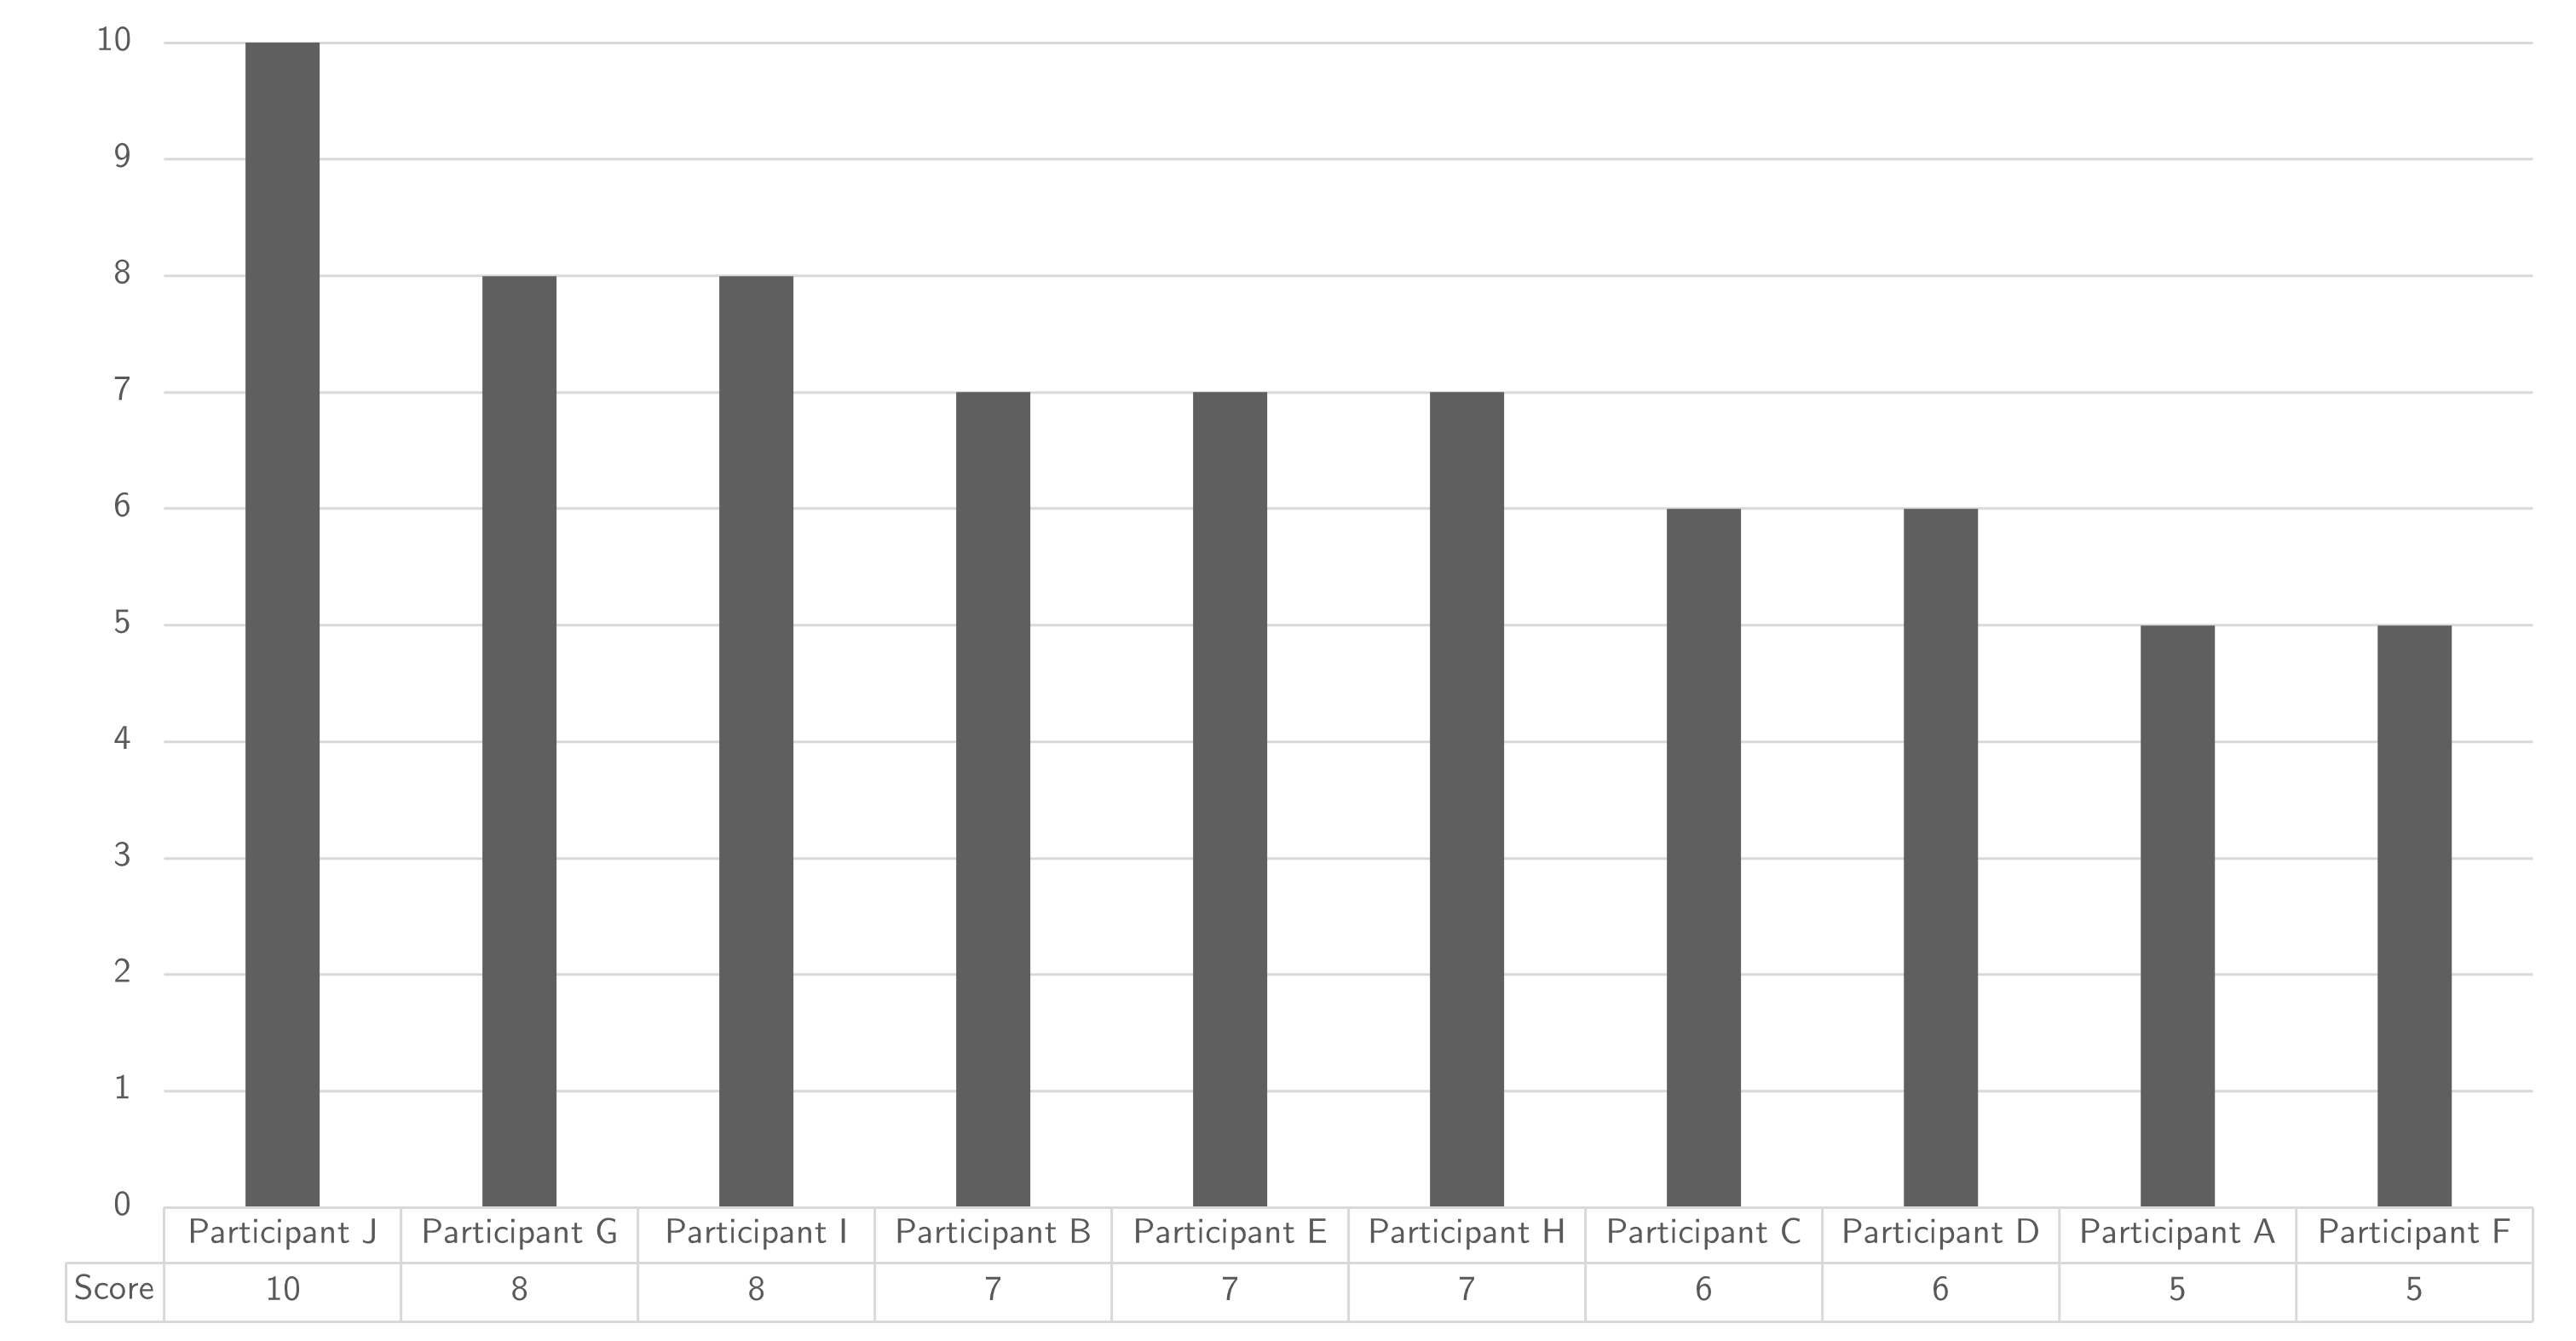
\includegraphics[width=0.9\linewidth]{images/scoreafoptionality}
	\caption[Rating of antifragile attribute Optionality]{Rating of antifragile attribute Optionality}
	\label{fig:appscoringafoptionality}
\end{figure}
\begin{table}[H]
	\centering
	\begin{tabular}{p{.55\textwidth}ccc}
		\toprule
		\textbf{Attribute} & \textbf{Rating} & \textbf{Variability} & \textbf{Abstains} \\
		\midrule
		Optionality & 6,9 & 32\% & 0 \\%
		\bottomrule
	\end{tabular}%
	\caption[Rating of antifragile attribute Optionality]{Rating of antifragile attribute Optionality}
	\label{tab:appscoringafoptionality}%
\end{table}%
\newpage
\subsection{Validation of non-monotonicity}
\begin{figure}[H]
	\centering
	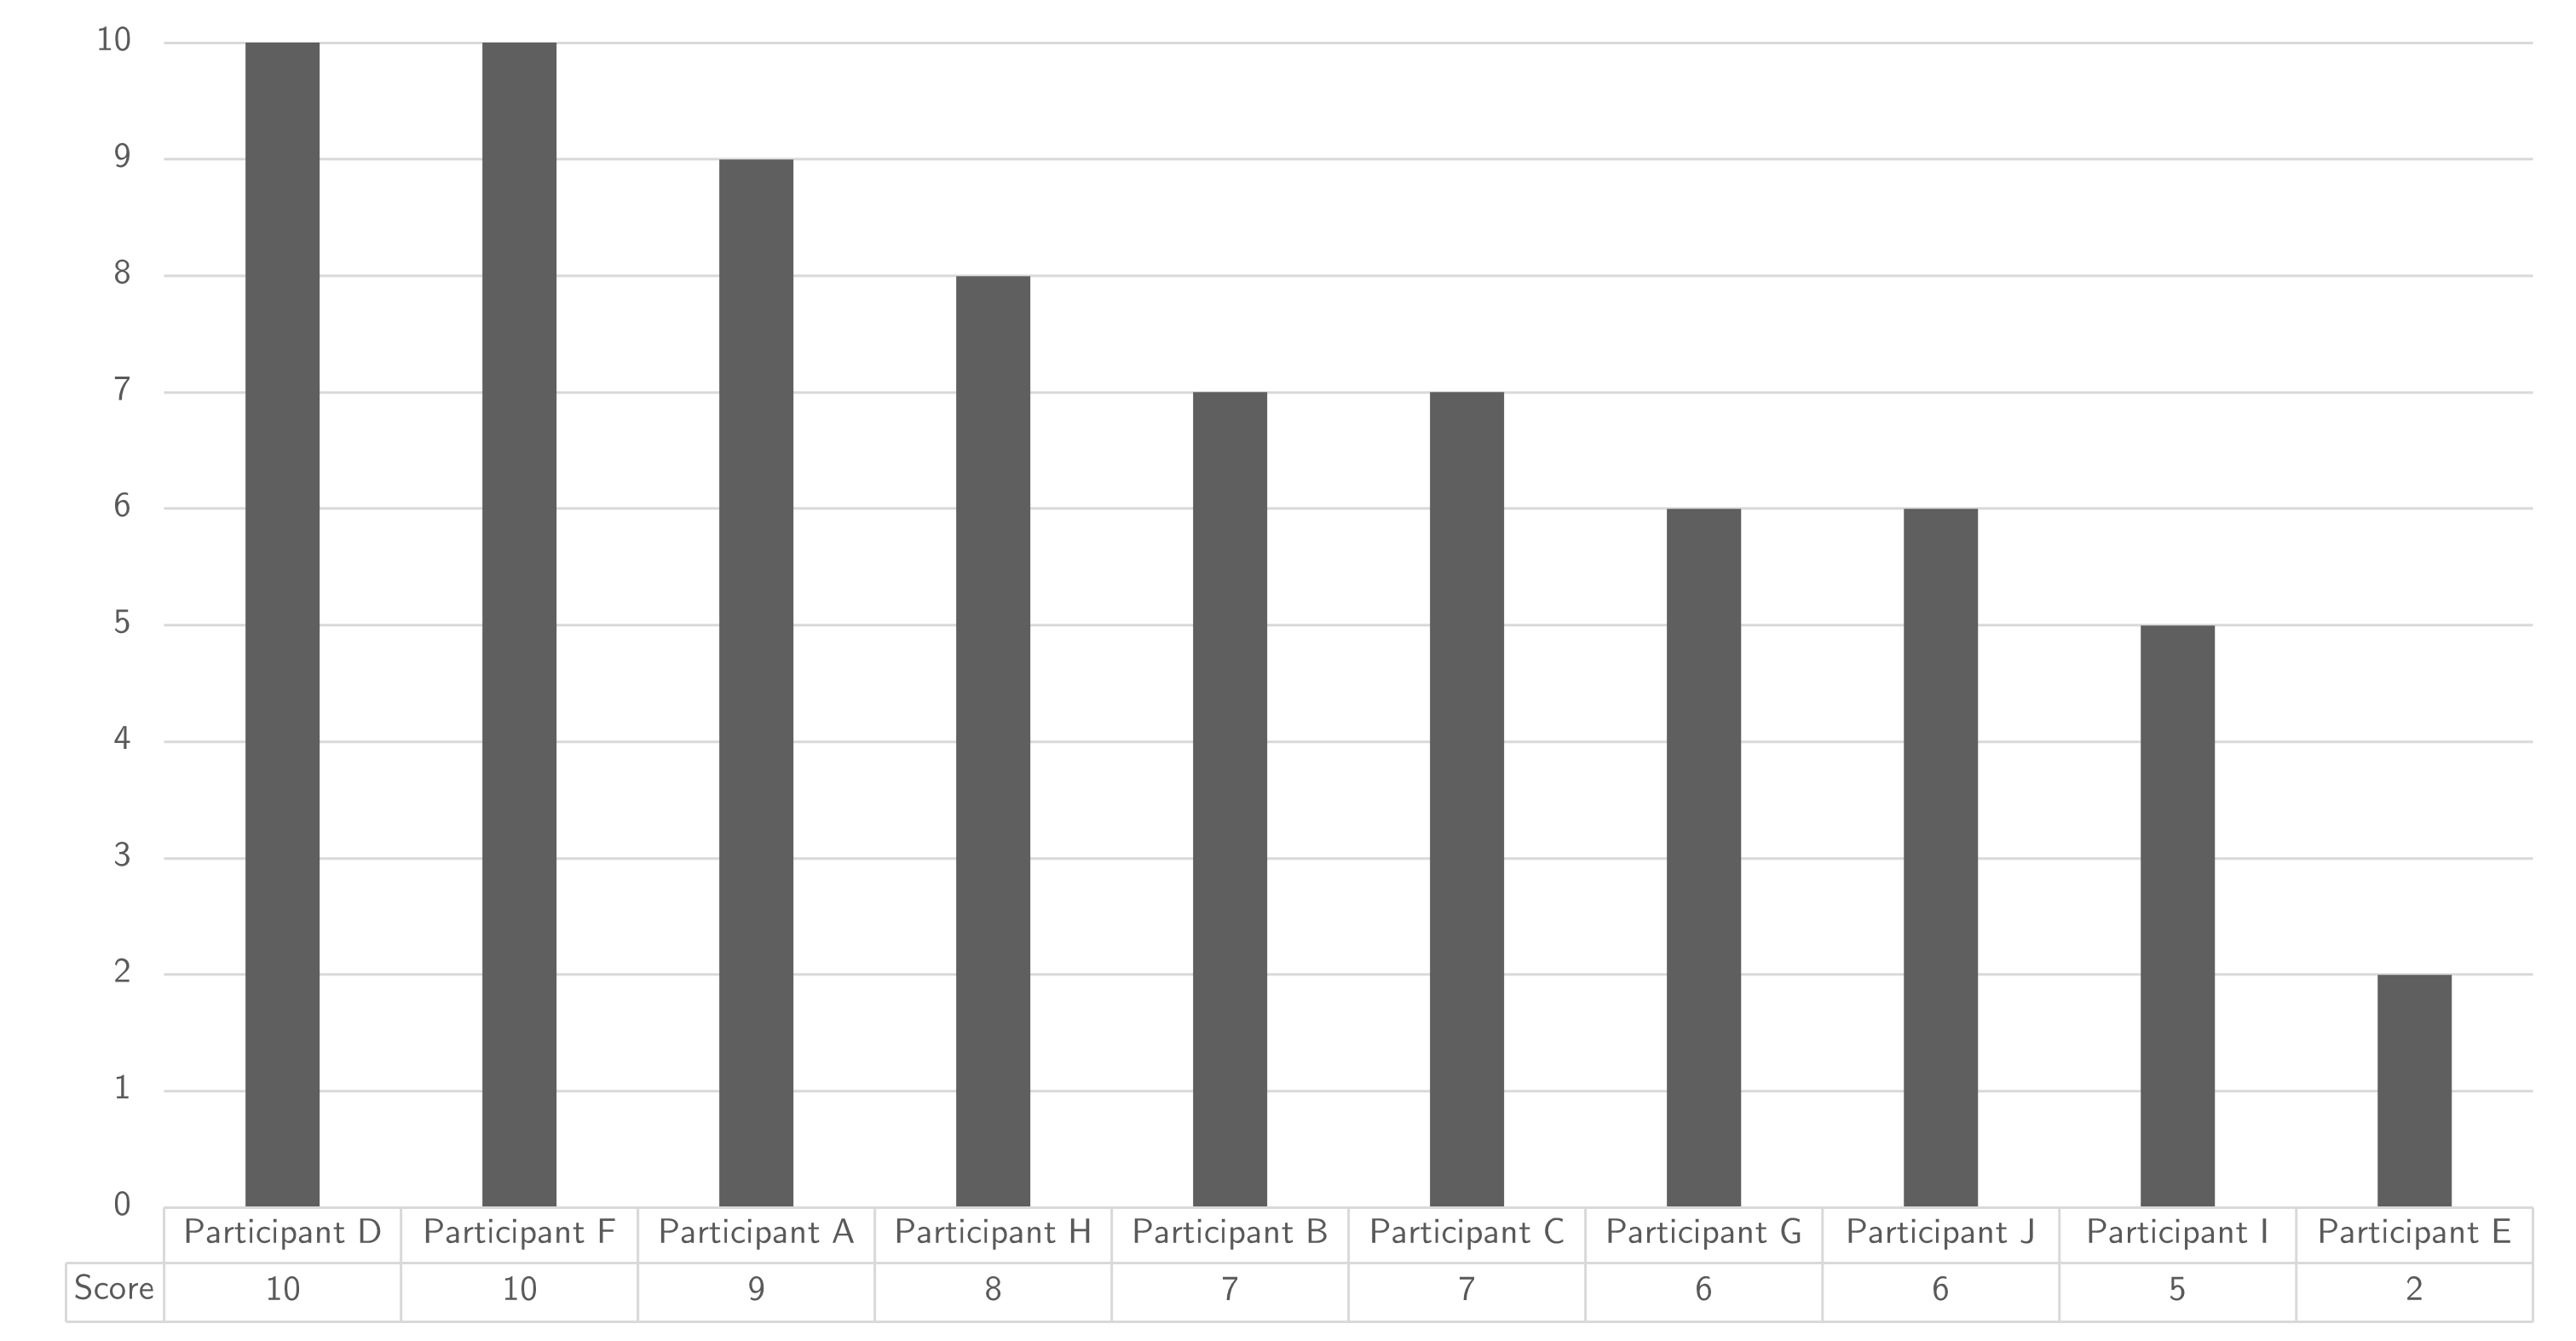
\includegraphics[width=0.9\linewidth]{images/scoreafmonomonotonicity}
	\caption[Scoring of antifragile attribute Mono-Monotonicity]{Scoring of antifragile attribute Mono-Monotonicity}
	\label{fig:appscoringafmonomonotonicity}
\end{figure}
\begin{table}[H]
	\centering
	\begin{tabular}{p{.55\textwidth}ccc}
		\toprule
		\textbf{Attribute} & \textbf{Rating} & \textbf{Variability} & \textbf{Abstains} \\
		\midrule
		Mono-Monotonicity & 7 & 51\% & 0 \\%
		\bottomrule
	\end{tabular}%
	\caption[Scoring of antifragile attribute Mono-Monotonicity]{Scoring of antifragile attribute Mono-Monotonicity}
	\label{tab:appscoringafmonomonotonicity}%
\end{table}%
\newpage
\subsection{Self-Organisation}
\begin{figure}[H]
	\centering
	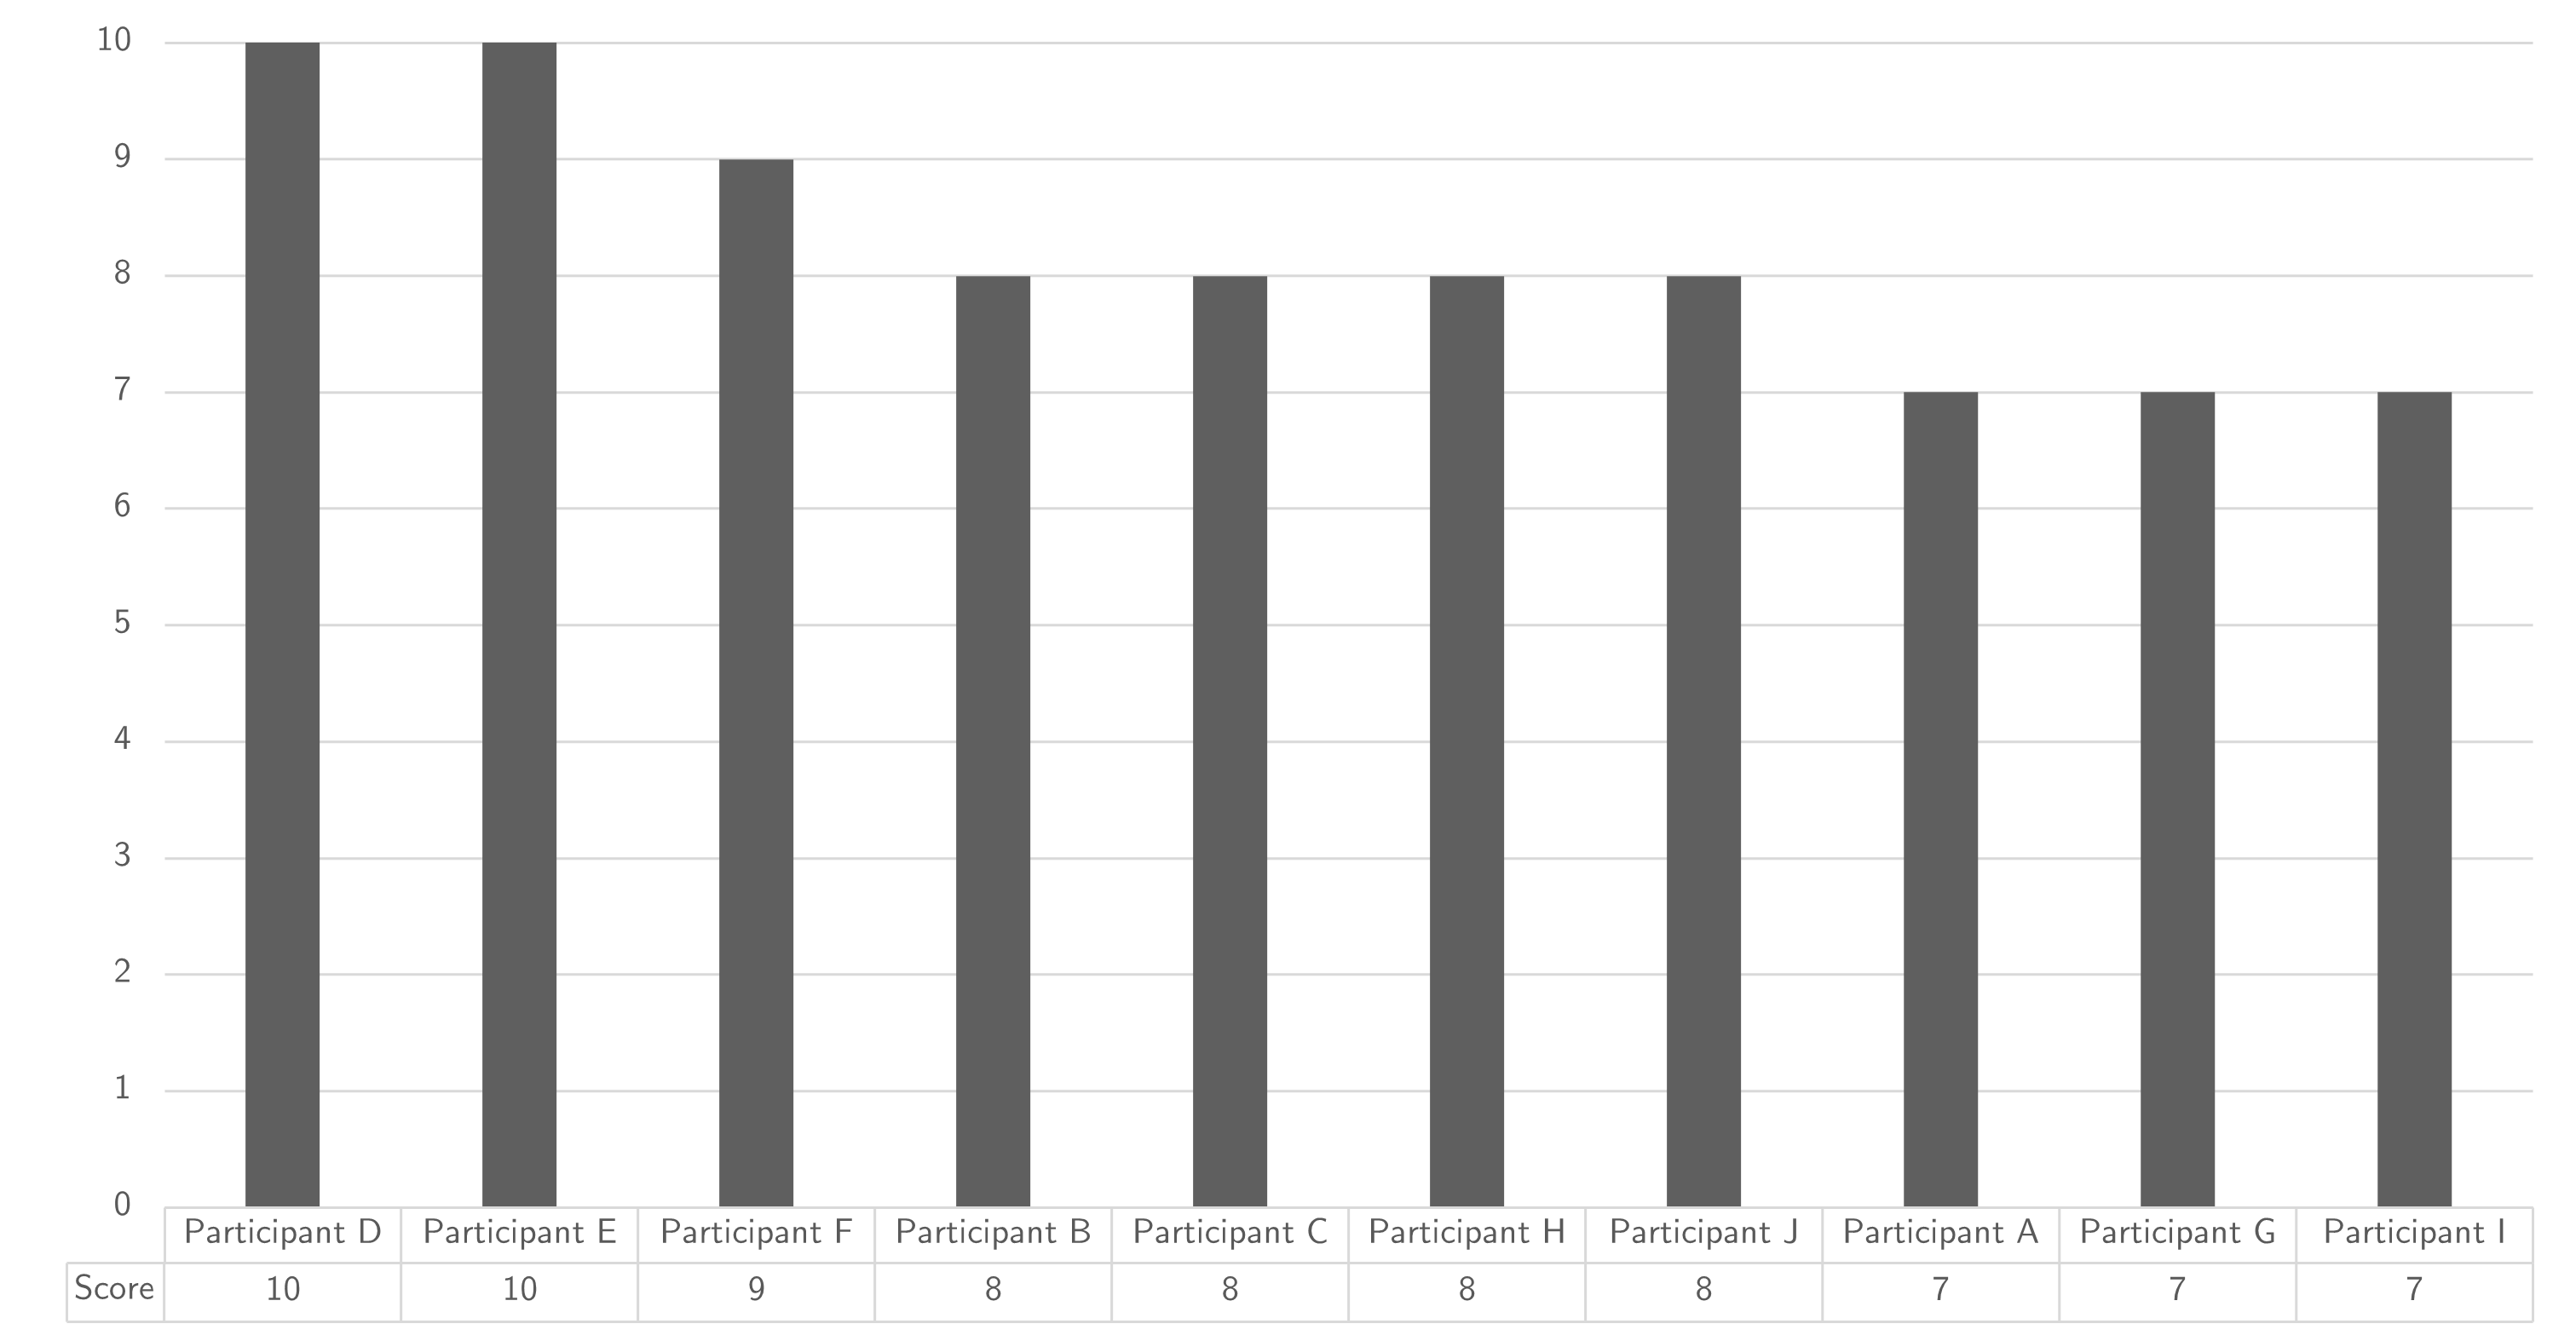
\includegraphics[width=0.9\linewidth]{images/scoreafselforganisation}
	\caption[Scoring of antifragile attribute Self-Organisation]{Scoring of antifragile attribute Self-Organisation}
	\label{fig:appscoringafselforganisation}
\end{figure}
\begin{table}[H]
	\centering
	\begin{tabular}{p{.55\textwidth}ccc}
		\toprule
		\textbf{Attribute} & \textbf{Rating} & \textbf{Variability} & \textbf{Abstains} \\
		\midrule
		Self-Organisation & 8,2 & 23\% & 0 \\%
		\bottomrule
	\end{tabular}%
	\caption[Scoring of antifragile attribute Self-Organisation]{Scoring of antifragile attribute Self-Organisation}
	\label{tab:appscoringafselforganisation}%
\end{table}%
\newpage
\subsection{Fail-Fast}
\begin{figure}[H]
	\centering
	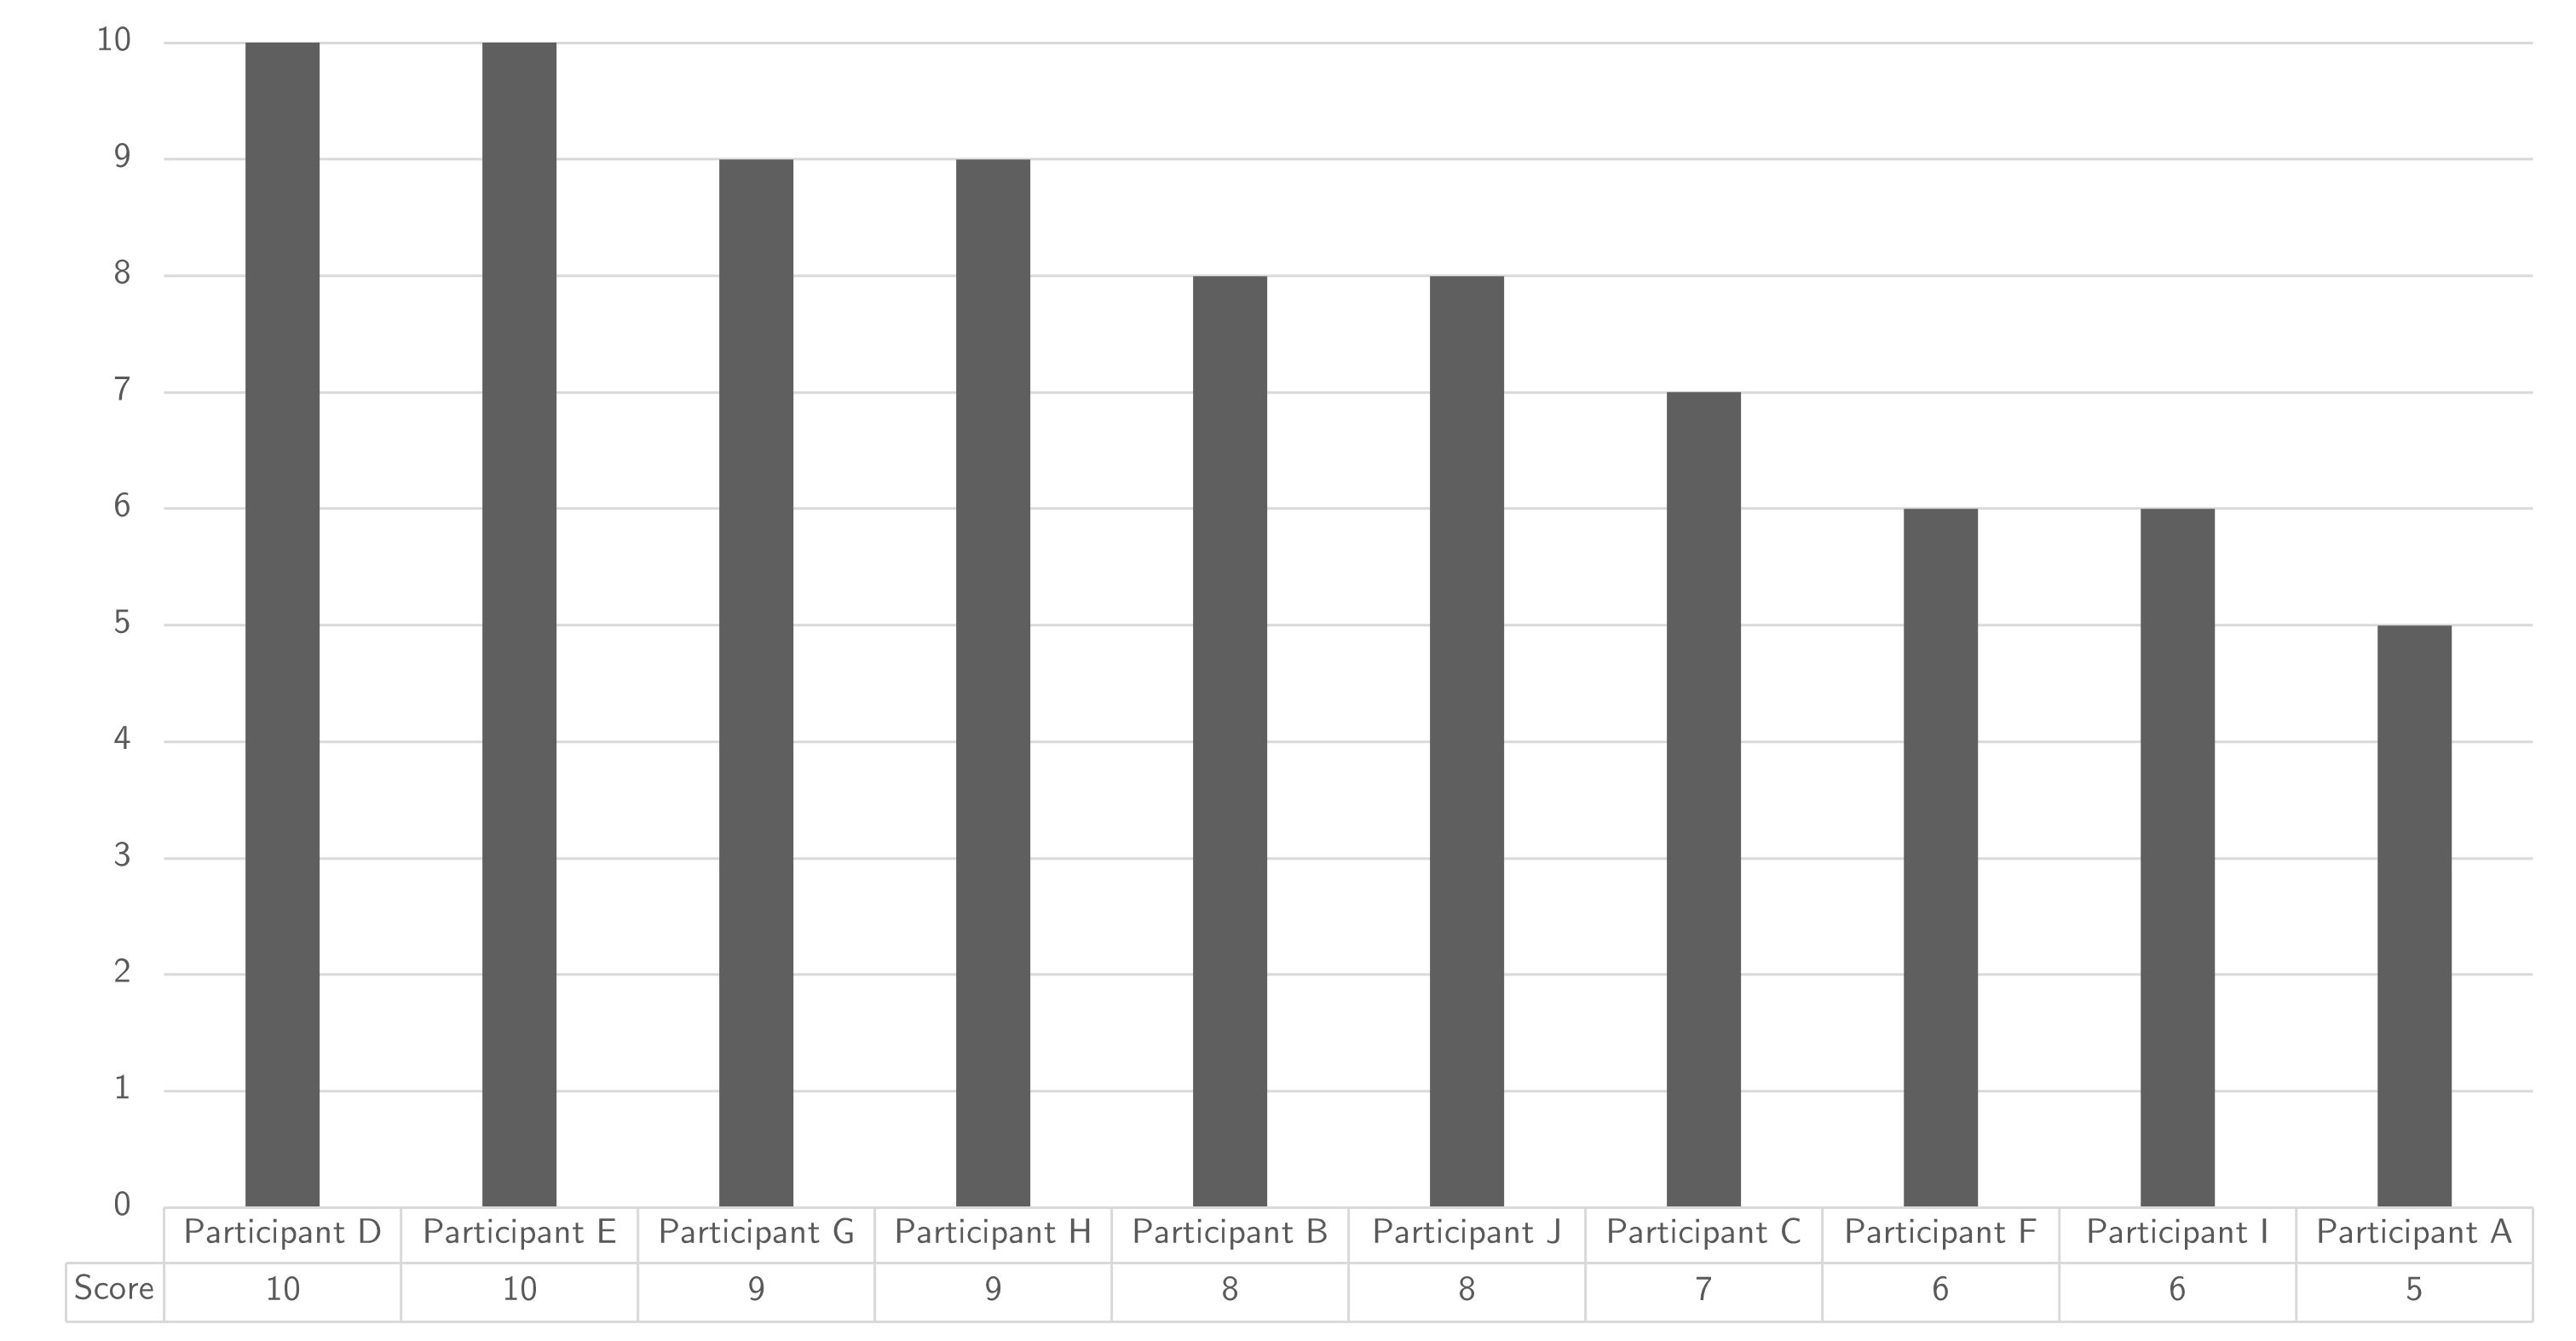
\includegraphics[width=0.9\linewidth]{images/scoreaffailfast}
	\caption[Scoring of antifragile attribute Fail-Fast]{Scoring of antifragile attribute Fail-Fast}
	\label{fig:appscoringaffailfast}
\end{figure}
\begin{table}[H]
	\centering
	\begin{tabular}{p{.55\textwidth}ccc}
		\toprule
		\textbf{Attribute} & \textbf{Rating} & \textbf{Variability} & \textbf{Abstains} \\
		\midrule
		Fail-Fast & 7,8 & 35\% & 0 \\%
		\bottomrule
	\end{tabular}%
	\caption[Scoring of antifragile attribute Fail-Fast]{Scoring of antifragile attribute Fail-Fast}
	\label{tab:appscoringaffailfast}%
\end{table}%
\newpage
\subsection{Resources to invest}
\begin{figure}[H]
	\centering
	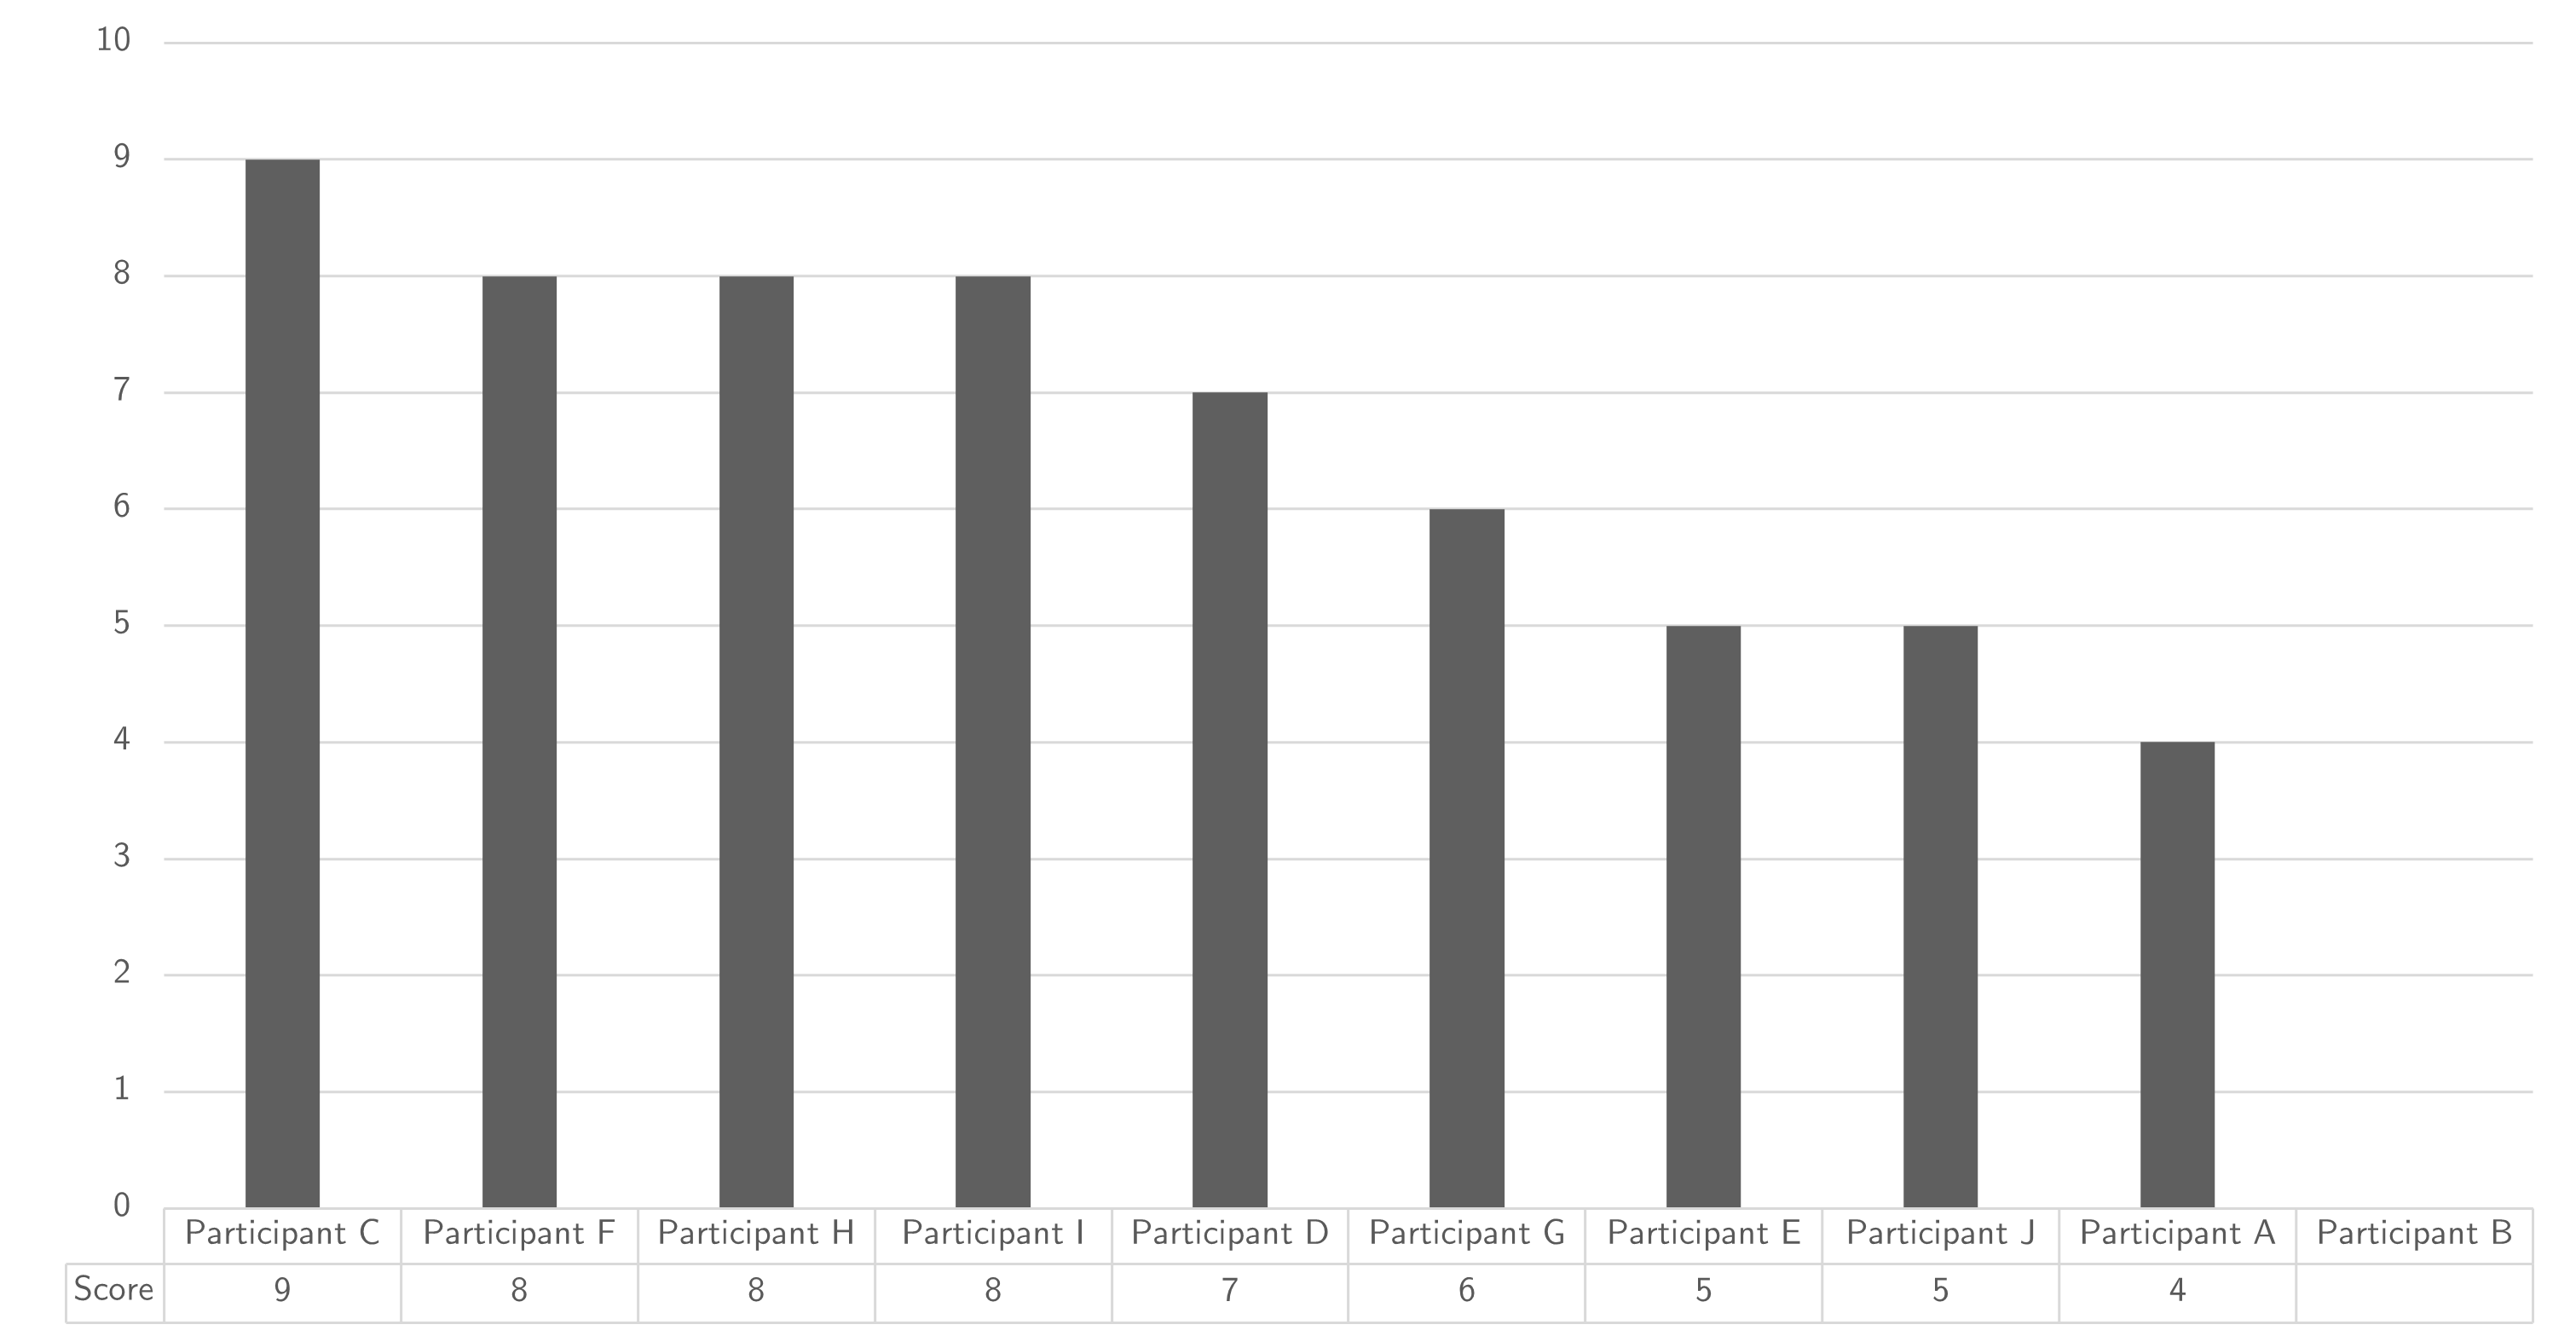
\includegraphics[width=0.9\linewidth]{images/scoreafresourcestoinvest}
	\caption[Scoring of antifragile attribute Resources to Invest]{Scoring of antifragile attribute Resources to Invest}
	\label{fig:appscoringafresourcestoinvest}
\end{figure}
\begin{table}[H]
	\centering
	\begin{tabular}{p{.55\textwidth}ccc}
		\toprule
		\textbf{Attribute} & \textbf{Rating} & \textbf{Variability} & \textbf{Abstains} \\
		\midrule
		Resources to Invest & 6,7 & 36\% & 1 \\%
		\bottomrule
	\end{tabular}%
	\caption[Scoring of antifragile attribute Resources to Invest]{Scoring of antifragile attribute Resources to Invest}
	\label{tab:appscoringafresourcestoinvest}%
\end{table}%
\newpage
\subsection{Senenca's Barbell}
\begin{figure}[H]
	\centering
	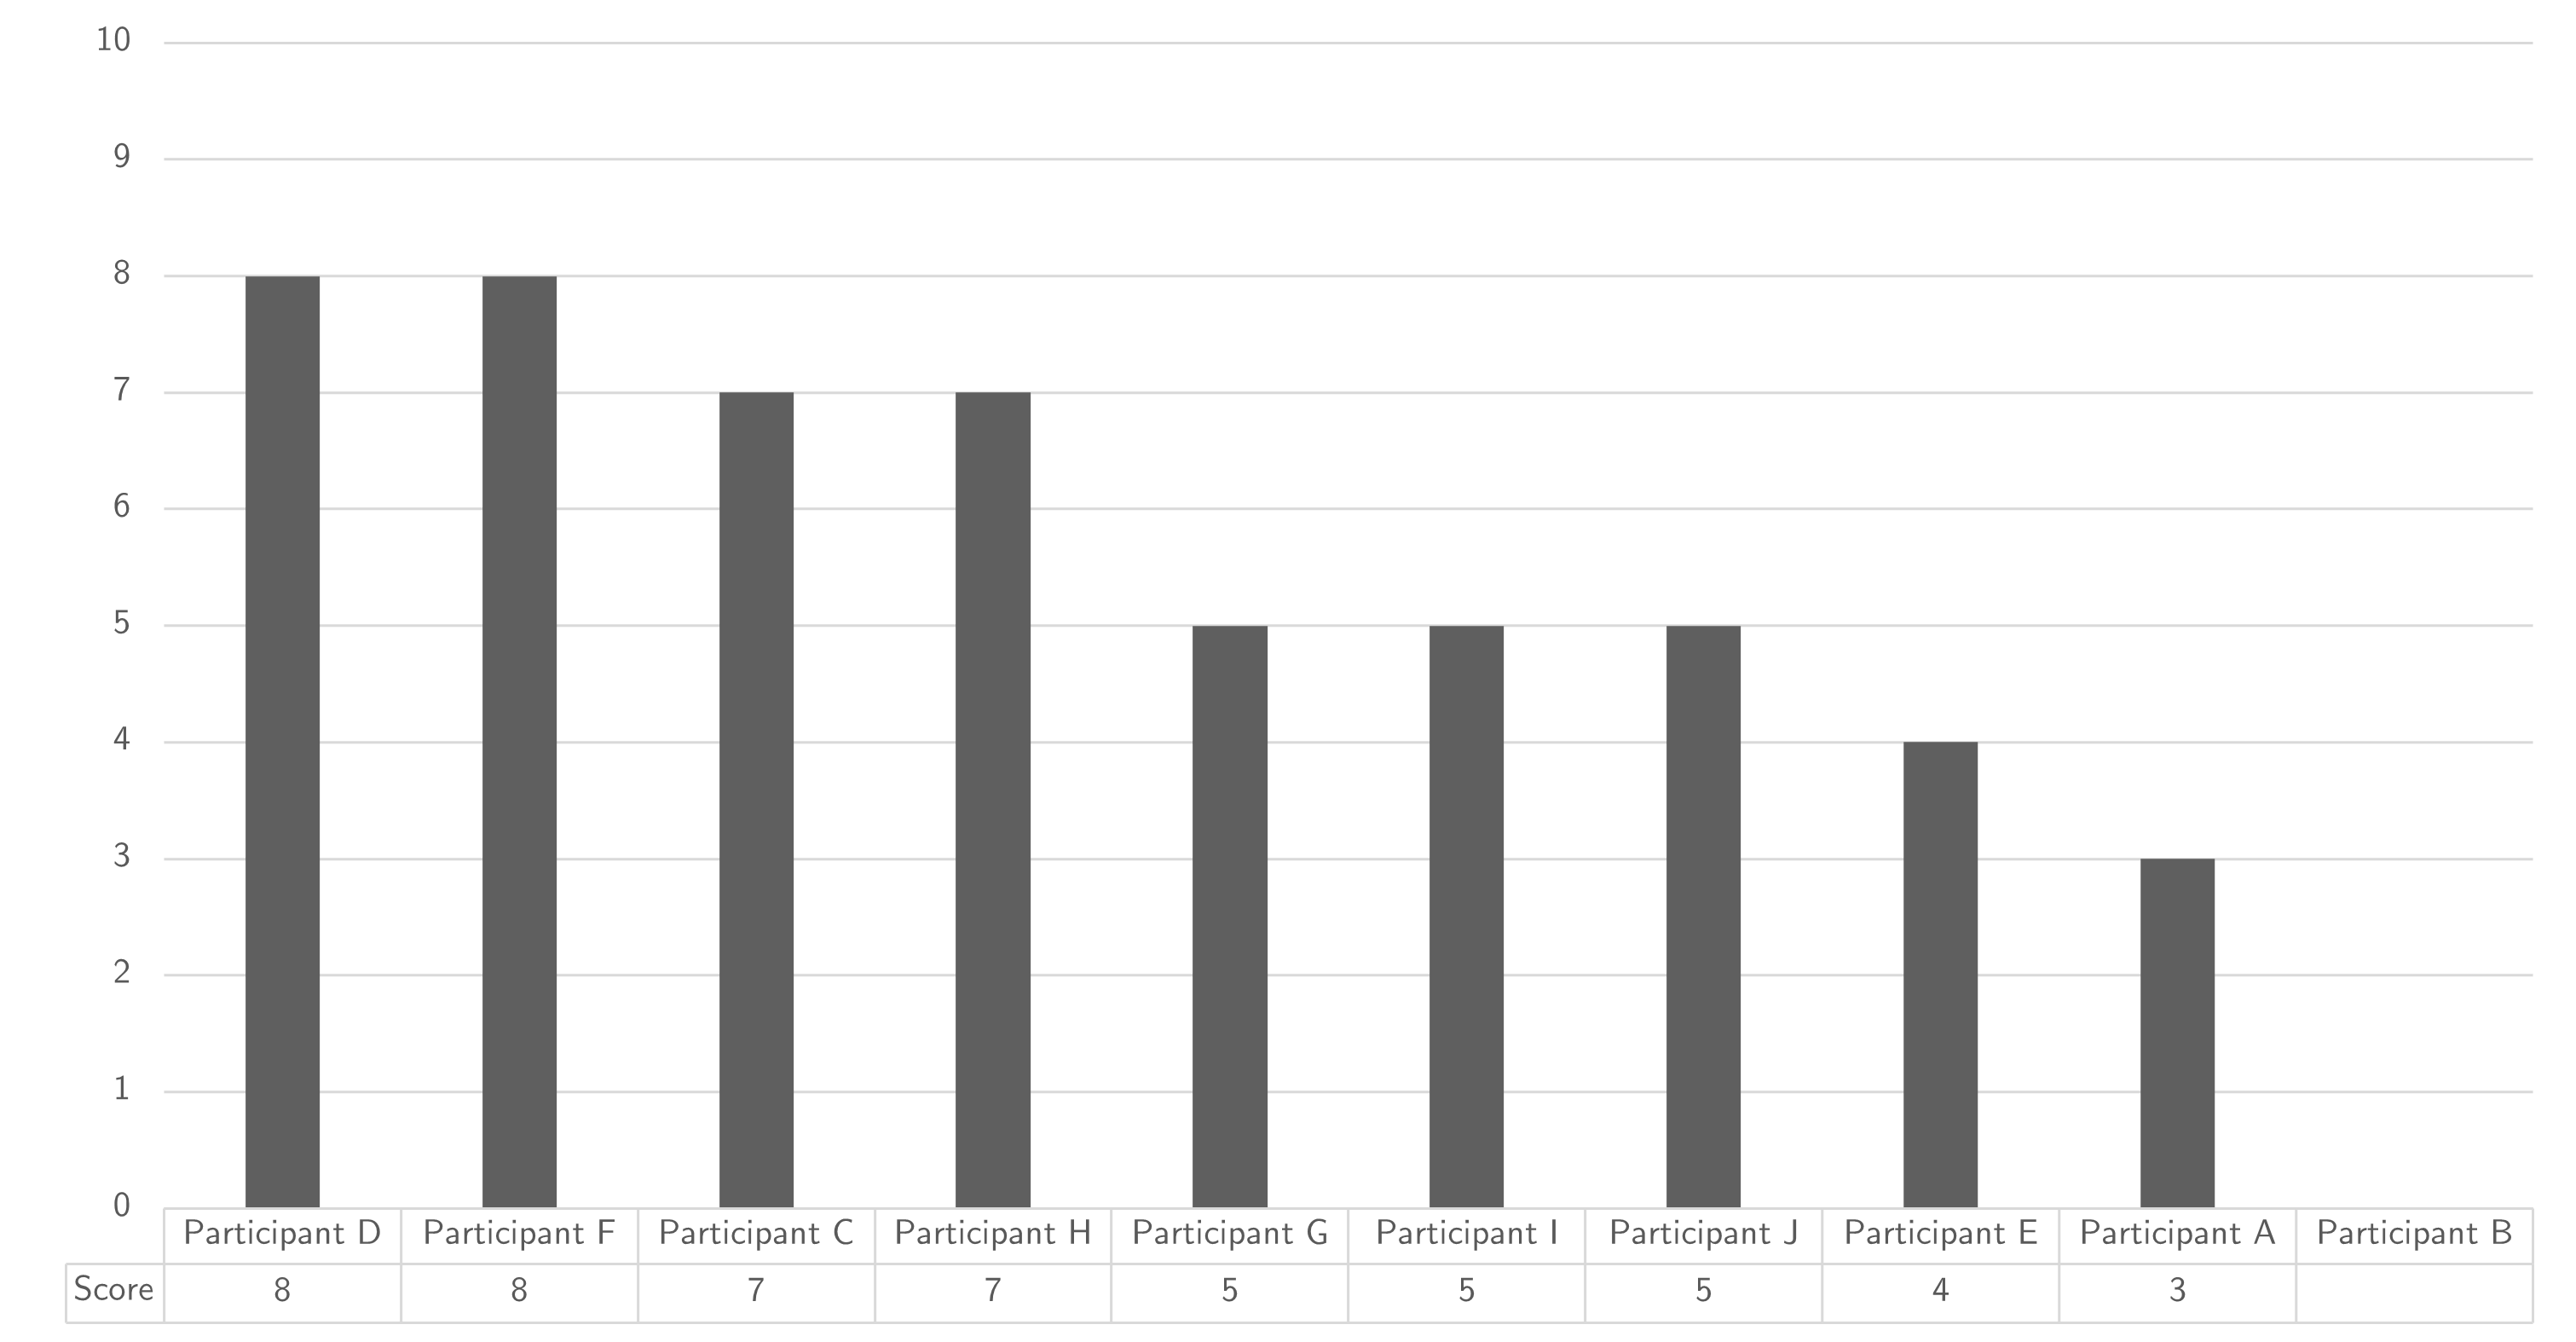
\includegraphics[width=0.9\linewidth]{images/scoreafseneca}
	\caption[Scoring of antifragile attribute Seneca's Barbell]{Scoring of antifragile attribute Seneca's Barbell}
	\label{fig:appscoringafseneca}
\end{figure}
\begin{table}[H]
	\centering
	\begin{tabular}{p{.55\textwidth}ccc}
		\toprule
		\textbf{Attribute} & \textbf{Rating} & \textbf{Variability} & \textbf{Abstains} \\
		\midrule
		Seneca's Barbell & 5,8 & 37\% & 1 \\%
		\bottomrule
	\end{tabular}%
	\caption[Scoring of antifragile attribute Seneca's Barbell]{Scoring of antifragile attribute Seneca's Barbell}
	\label{tab:appscoringafseneca}%
\end{table}%
\newpage
\subsection{Safe working environment}
\begin{figure}[H]
	\centering
	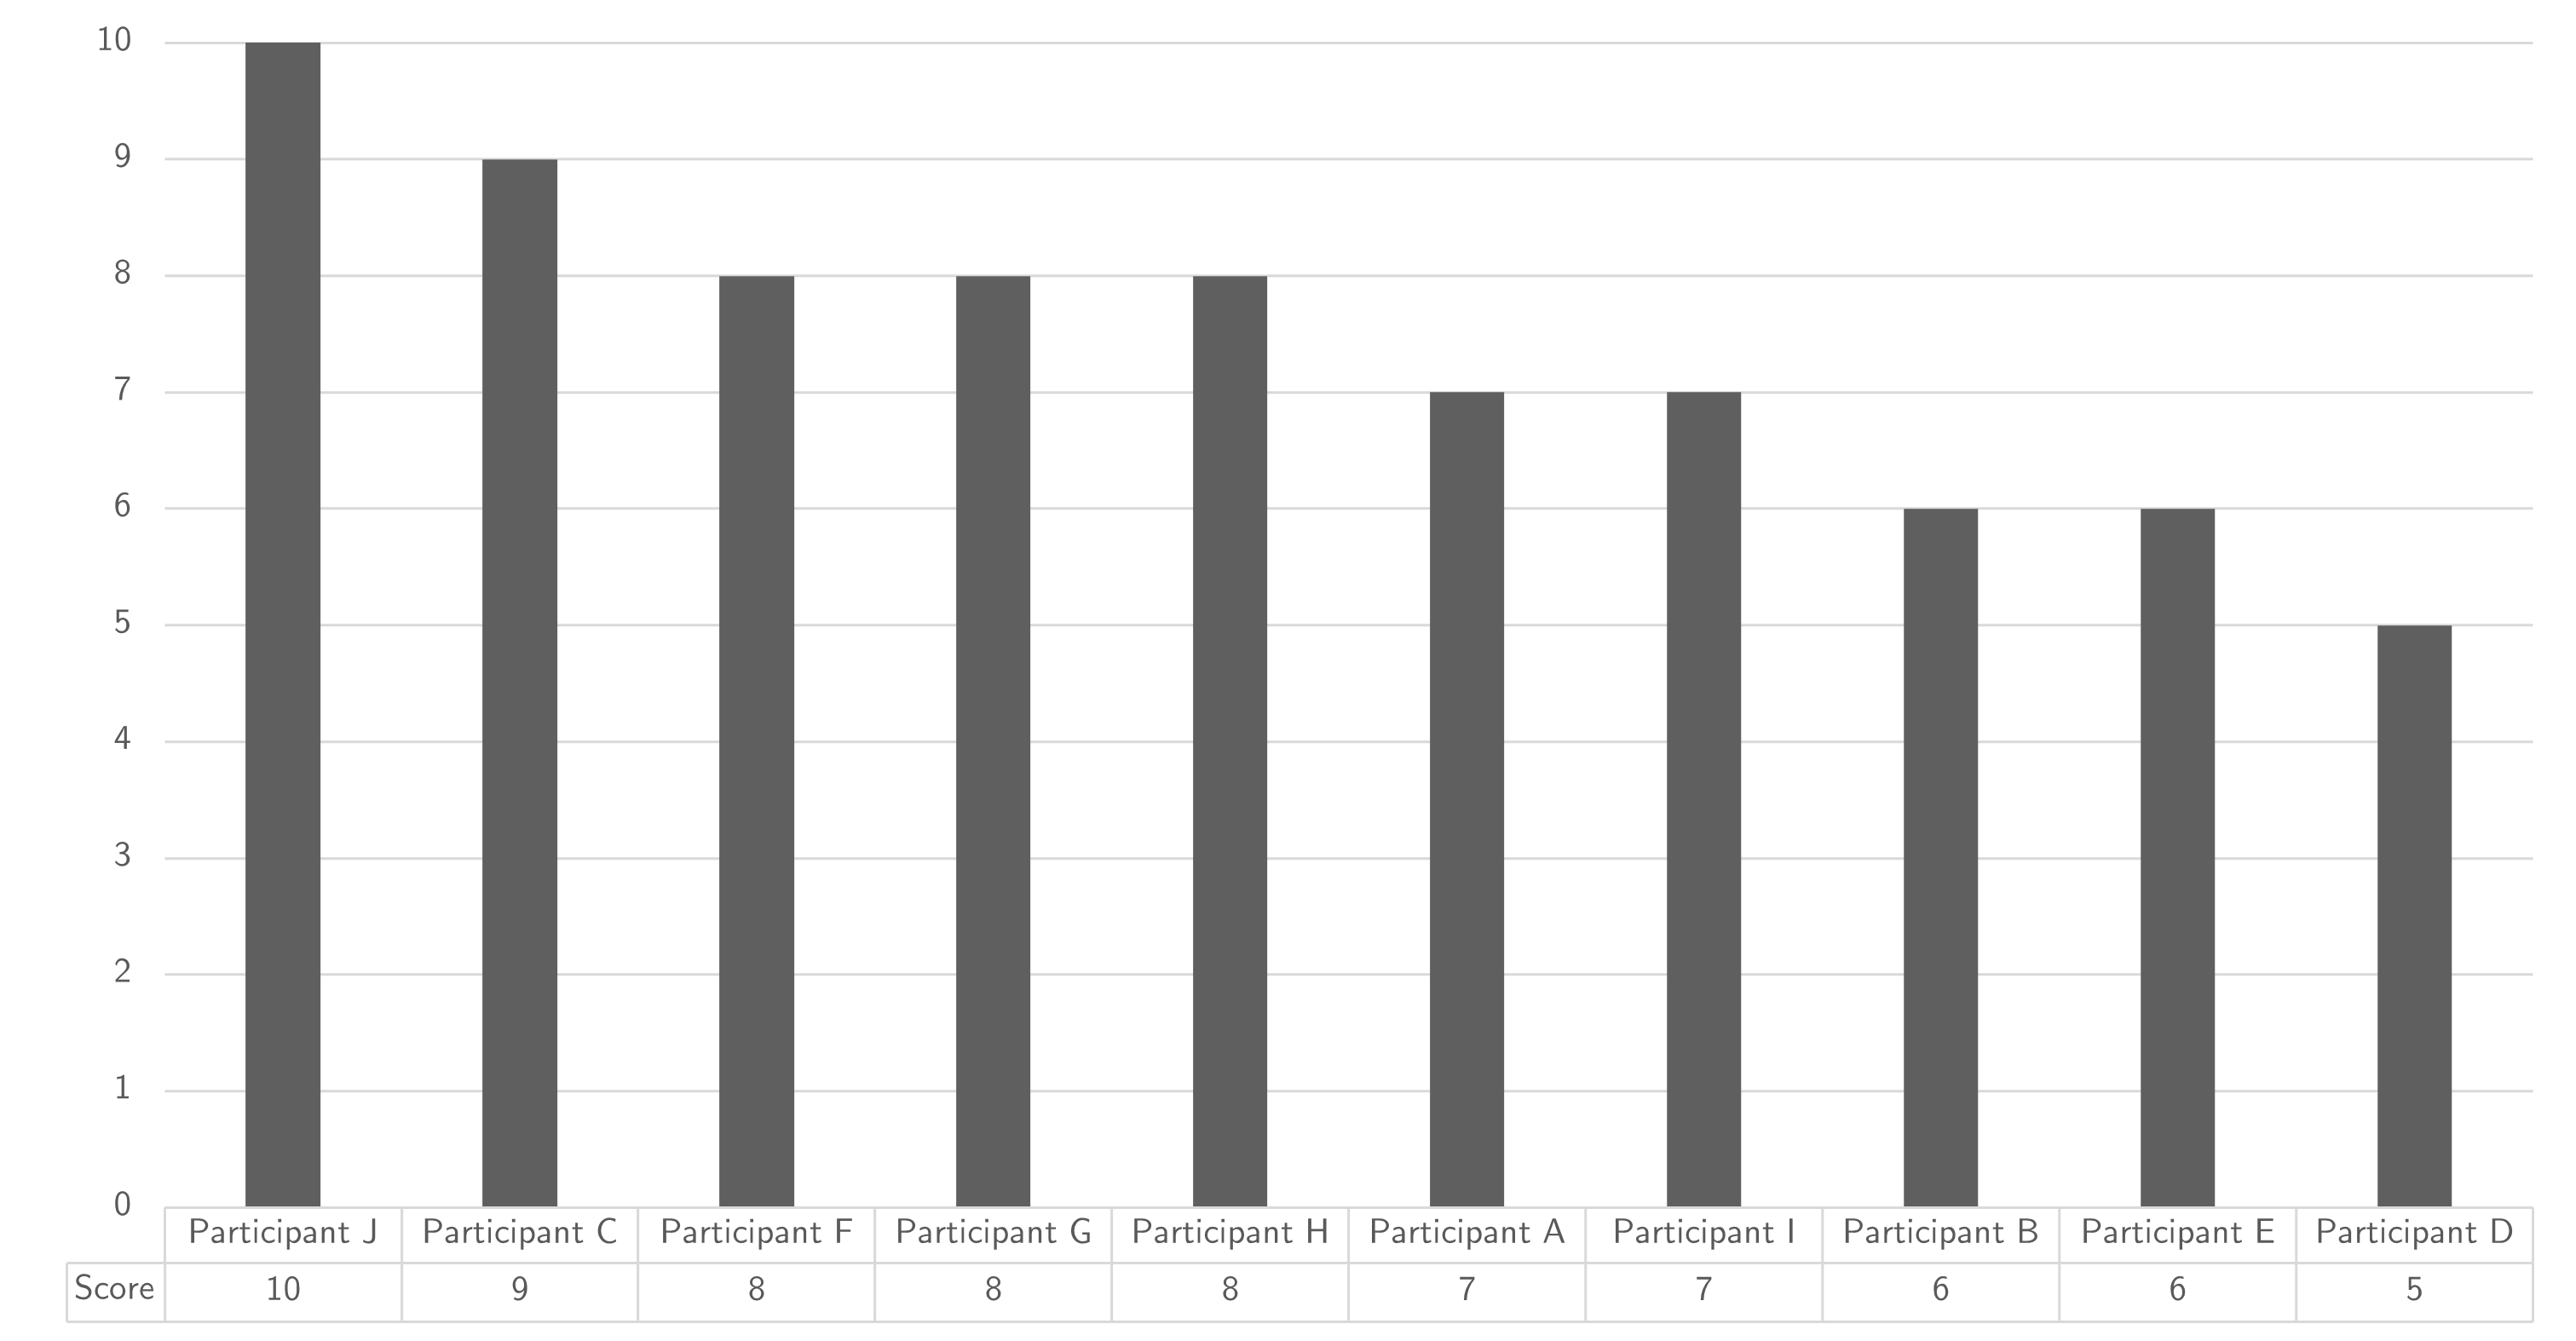
\includegraphics[width=0.9\linewidth]{images/scoreafsafeworkingenvironnment}
	\caption[Scoring of antifragile attribute Safe working environment]{Scoring of antifragile attribute Safe working environment}
	\label{fig:appscoringafsafeworkingenvironnment}
\end{figure}
\begin{table}[H]
	\centering
	\begin{tabular}{p{.55\textwidth}ccc}
		\toprule
		\textbf{Attribute} & \textbf{Rating} & \textbf{Variability} & \textbf{Abstains} \\
		\midrule
		Safe working environment & 7,4 & 31\% & 0 \\%
		\bottomrule
	\end{tabular}%
	\caption[Scoring of antifragile attribute Safe working environment]{Scoring of antifragile attribute Safe working environment}
	\label{tab:appscoringafsafeworkingenvironment}%
\end{table}%
\newpage
\subsection{Outside-In and Collaboration}
\begin{figure}[H]
	\centering
	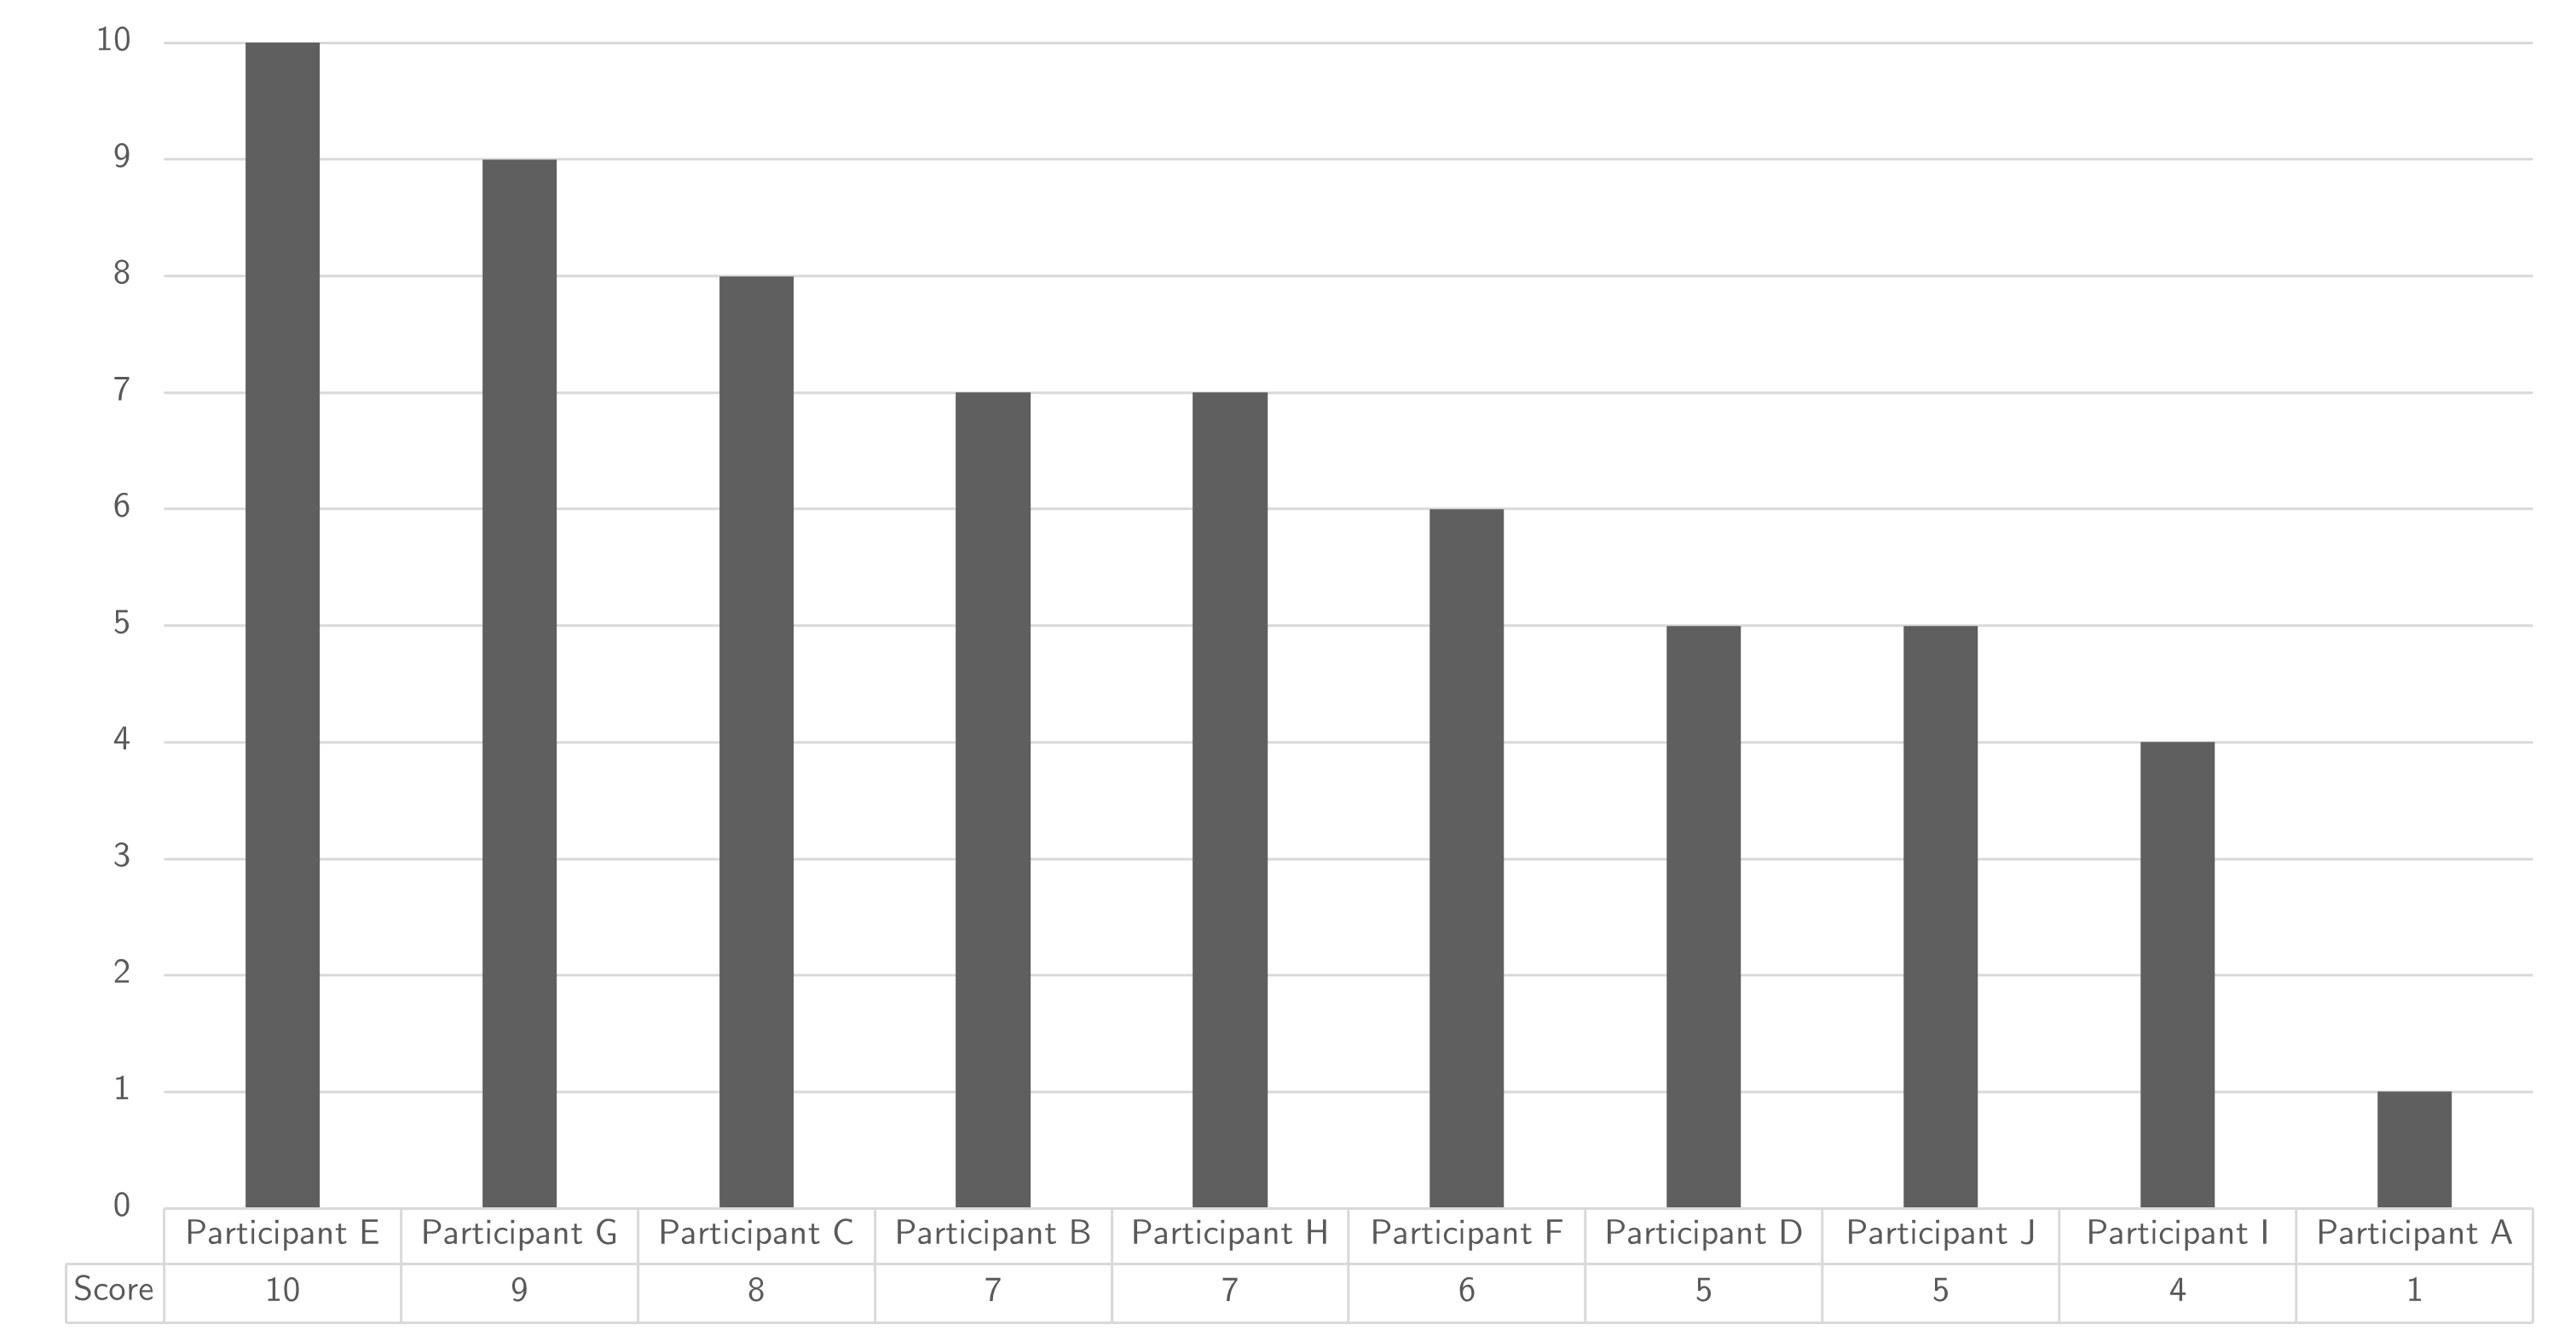
\includegraphics[width=0.9\linewidth]{images/scoreafnaarbuitenkijken}
	\caption[Scoring of antifragile attribute Outside-In and Collaboration]{Scoring of antifragile attribute Outside-In and Collaboration}
	\label{fig:appscoringafnaarbuiten}
\end{figure}
\begin{table}[H]
	\centering
	\begin{tabular}{p{.55\textwidth}ccc}
		\toprule
		\textbf{Attribute} & \textbf{Rating} & \textbf{Variability} & \textbf{Abstains} \\
		\midrule
		Naar buiten kijken, samenwerking zoeken & 6,2 & 55\% & 0 \\%
		\bottomrule
	\end{tabular}%
	\caption[Scoring of antifragile attribute Outside-In and Collaboration]{Scoring of antifragile attribute Outside-In and Collaboration}
	\label{tab:appscoringafnaarbuitenkijken}%
\end{table}%
\newpage
\subsection{Data Governance Planes}
\begin{figure}[H]
	\centering
	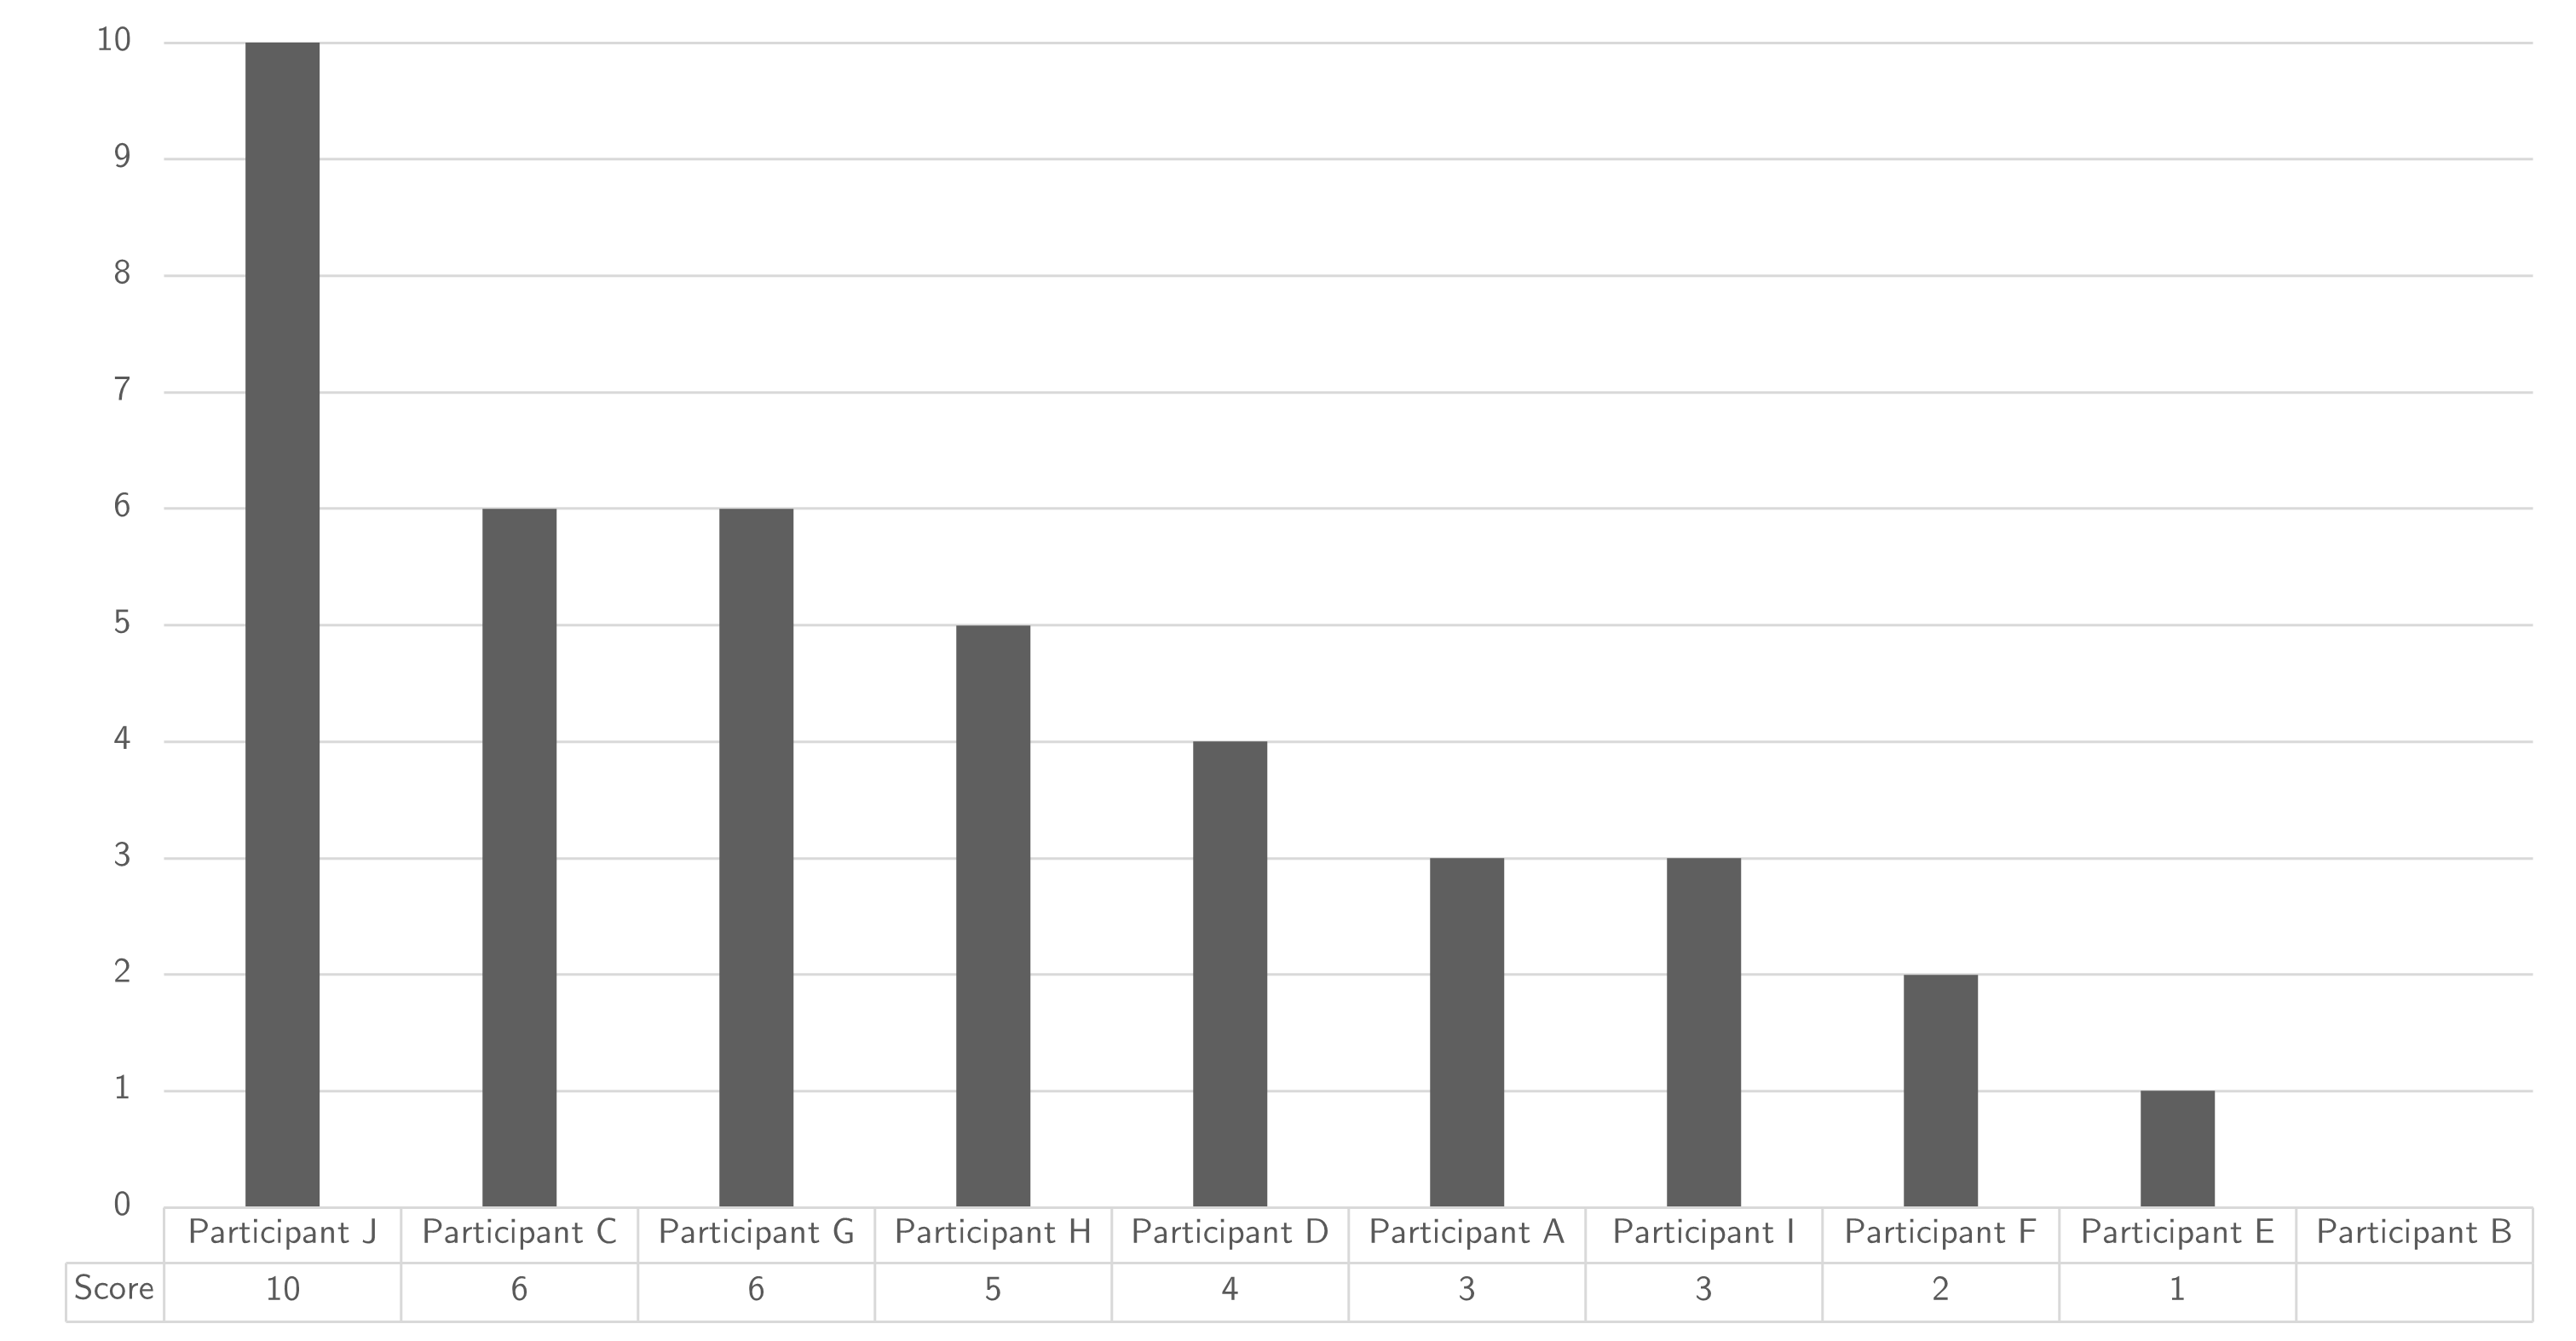
\includegraphics[width=0.9\linewidth]{images/scoreafdatagovernanceplanes}
	\caption[Scoring of antifragile attribute Data Governance Planes]{Scoring of antifragile attribute Data Governance Planes}
	\label{fig:appscoringafdatagovernanceplanes}
\end{figure}
\begin{table}[H]
	\centering
	\begin{tabular}{ccc}
		\toprule
		\textbf{Rating} & \textbf{Variability} & \textbf{Abstains} \\
		\midrule
		4,4 & 56\% & 1 \\%
		\bottomrule
	\end{tabular}%
	\caption[Scoring of antifragile attribute Data Governance Planes]{Scoring of antifragile attribute Data Governance Planes}
	\label{tab:appscoringafdatagovernance}
\end{table}%
\newpage
\section{Validation of Enterprise Architecture schools of thought}
\label{sec:validationofeaschools}
\begin{table}[H]
	\centering
	\begin{tabular}{p{.55\textwidth}ccc}
		\toprule
		\textbf{School} & \textbf{Rating} & \textbf{Variability} & \textbf{Abstains} \\
		\midrule
		Enterprise IT Architecting & 5,6 & 34\% & 0 \\%
		Enterprise Integrating & 7,2 & 16\% & 0 \\%
		Enterprise Ecological Adaptation & 8,8 & 27\% & 0 \\%
		\bottomrule
	\end{tabular}%
	\caption{Validation of Enterprise Architecture schools of thought}
	\label{tab:appvalidationofeaschools}%
\end{table}%
\subsection{Enterprise IT Architecting}
\begin{figure}[H]
	\centering
	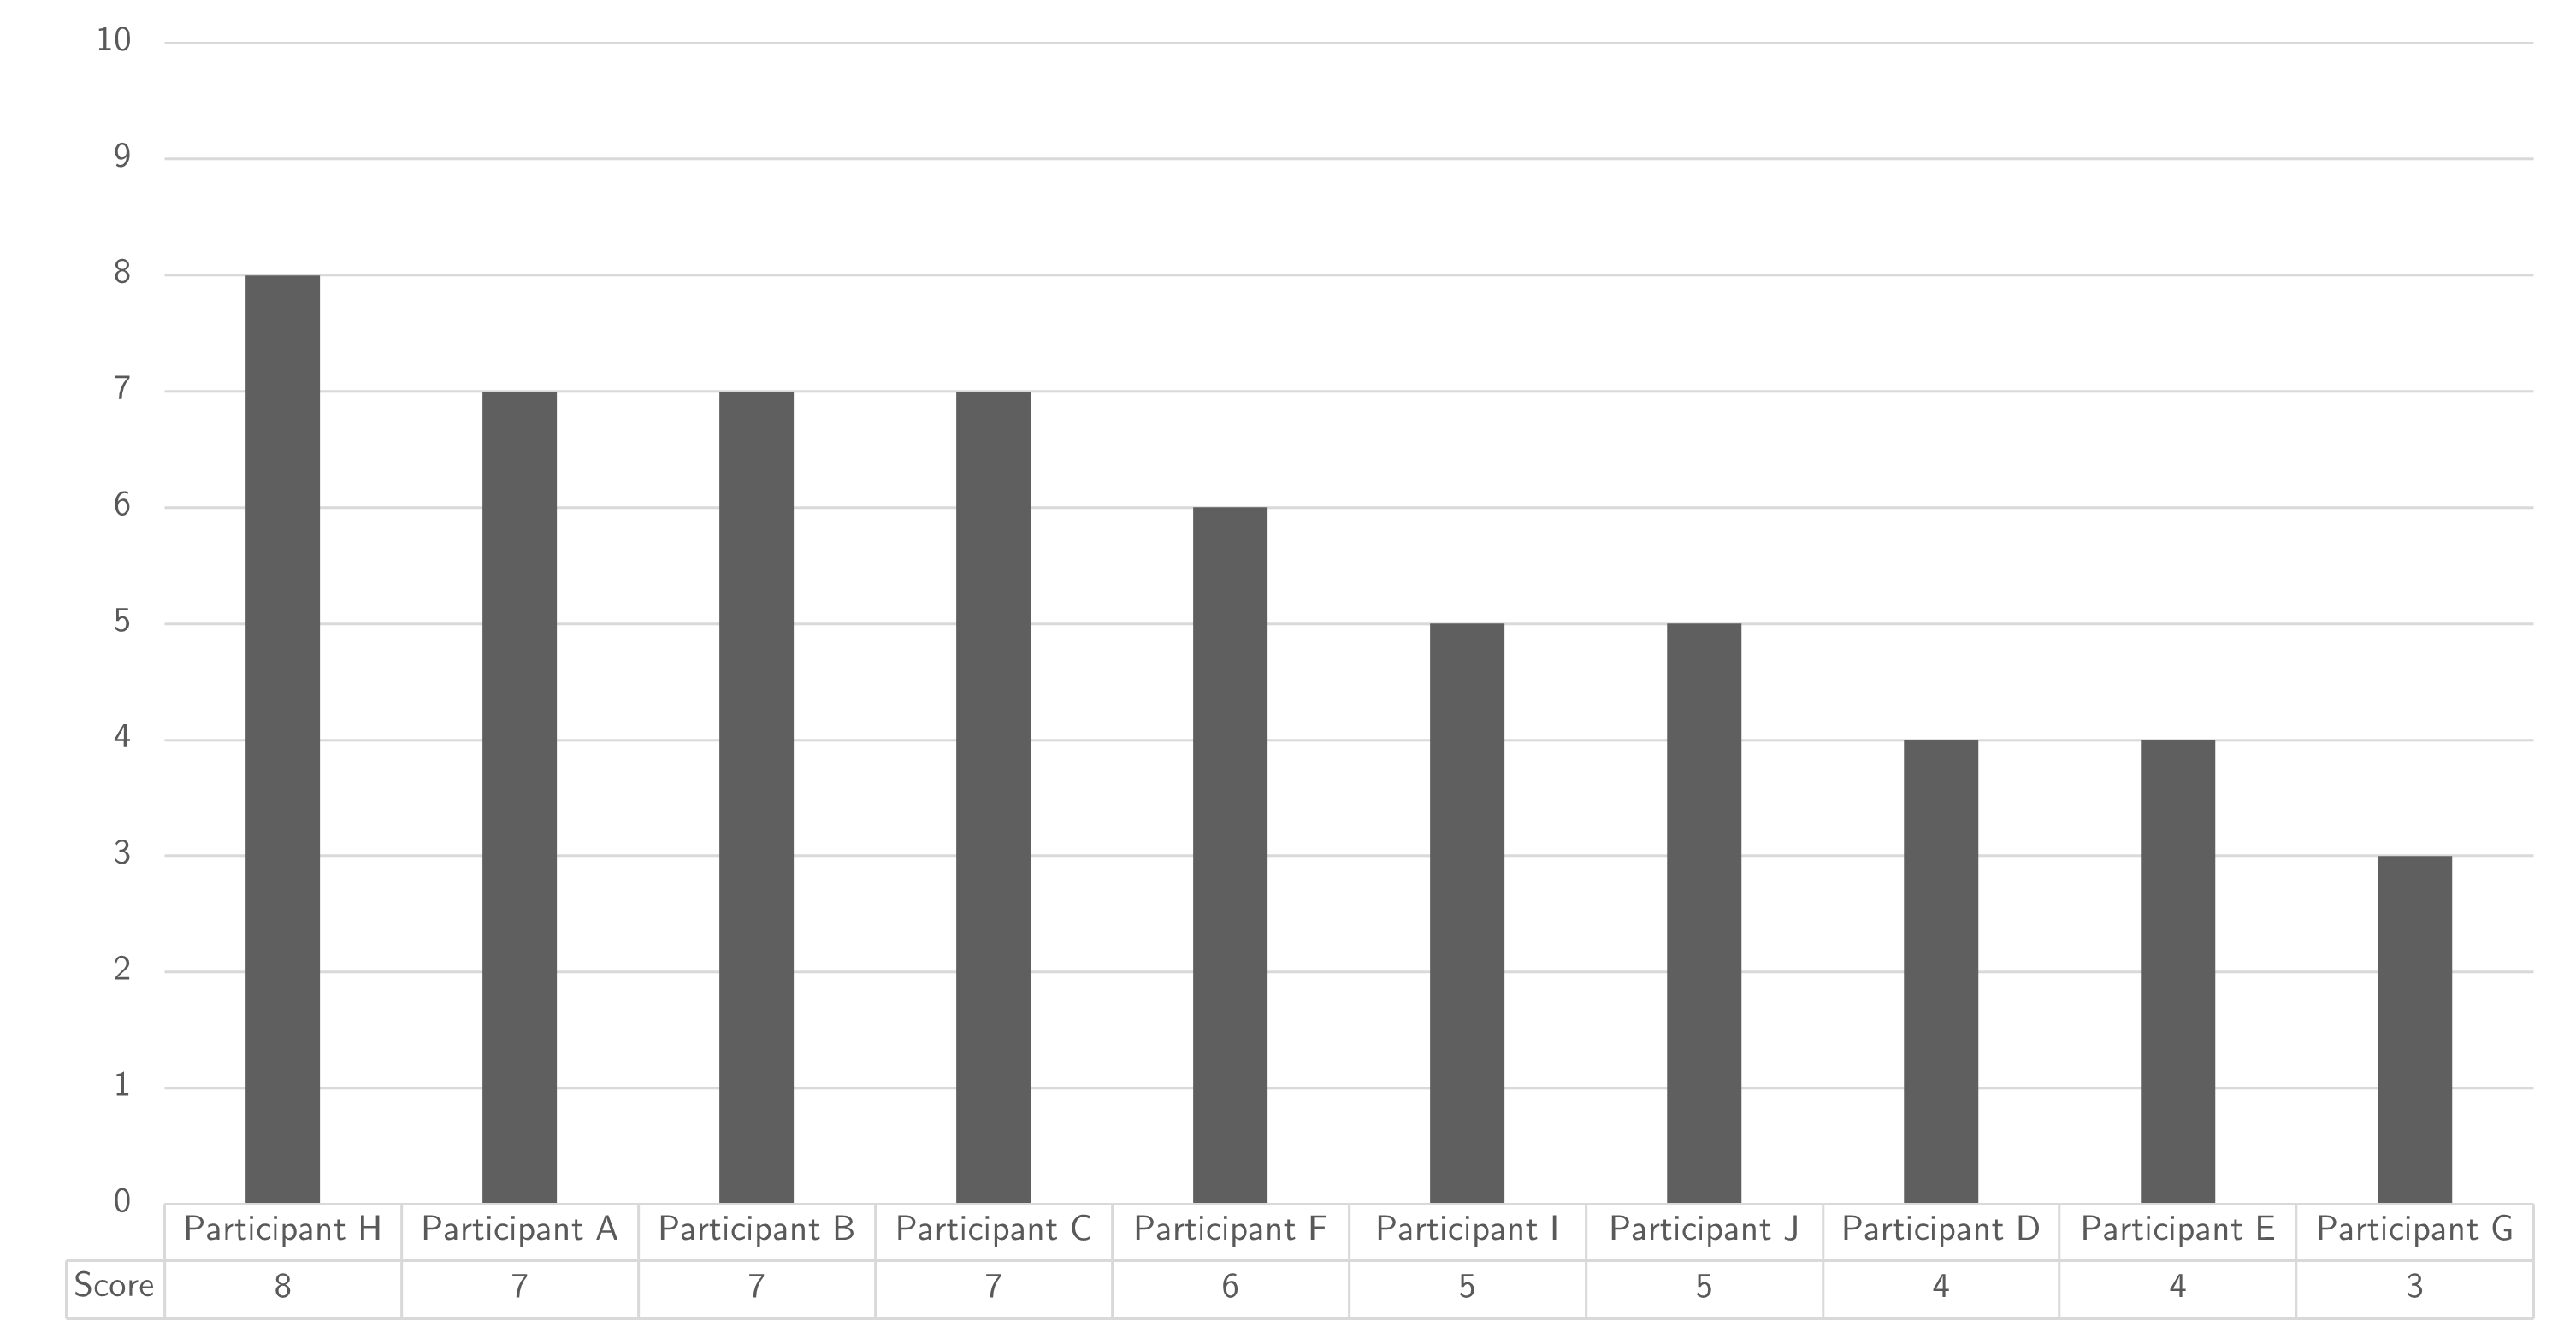
\includegraphics[width=0.9\linewidth]{images/scoreeaschoolenterpriseitarchitecting}
	\caption[Scoring of school of thought Enterprise IT Architecting]{Scoring of school of thought Enterprise IT Architecting}
	\label{fig:appscoringschoolenterpriseitarchitecting}
\end{figure}
\begin{table}[H]
	\centering
	\begin{tabular}{p{.55\textwidth}ccc}
		\toprule
		\textbf{Attribute} & \textbf{Rating} & \textbf{Variability} & \textbf{Abstains} \\
		\midrule
		Enterprise IT Architecting & 5,6 & 34\% & 0 \\%
		\bottomrule
	\end{tabular}%
	\caption[Scoring of school of thought Enterprise IT Architecting]{Scoring of school of thought Enterprise IT Architecting}
	\label{tab:appscoringschoolenterpriseitarchitecting}%
\end{table}%

\newpage
\subsection{Enterprise Integrating}
\begin{figure}[H]
	\centering
	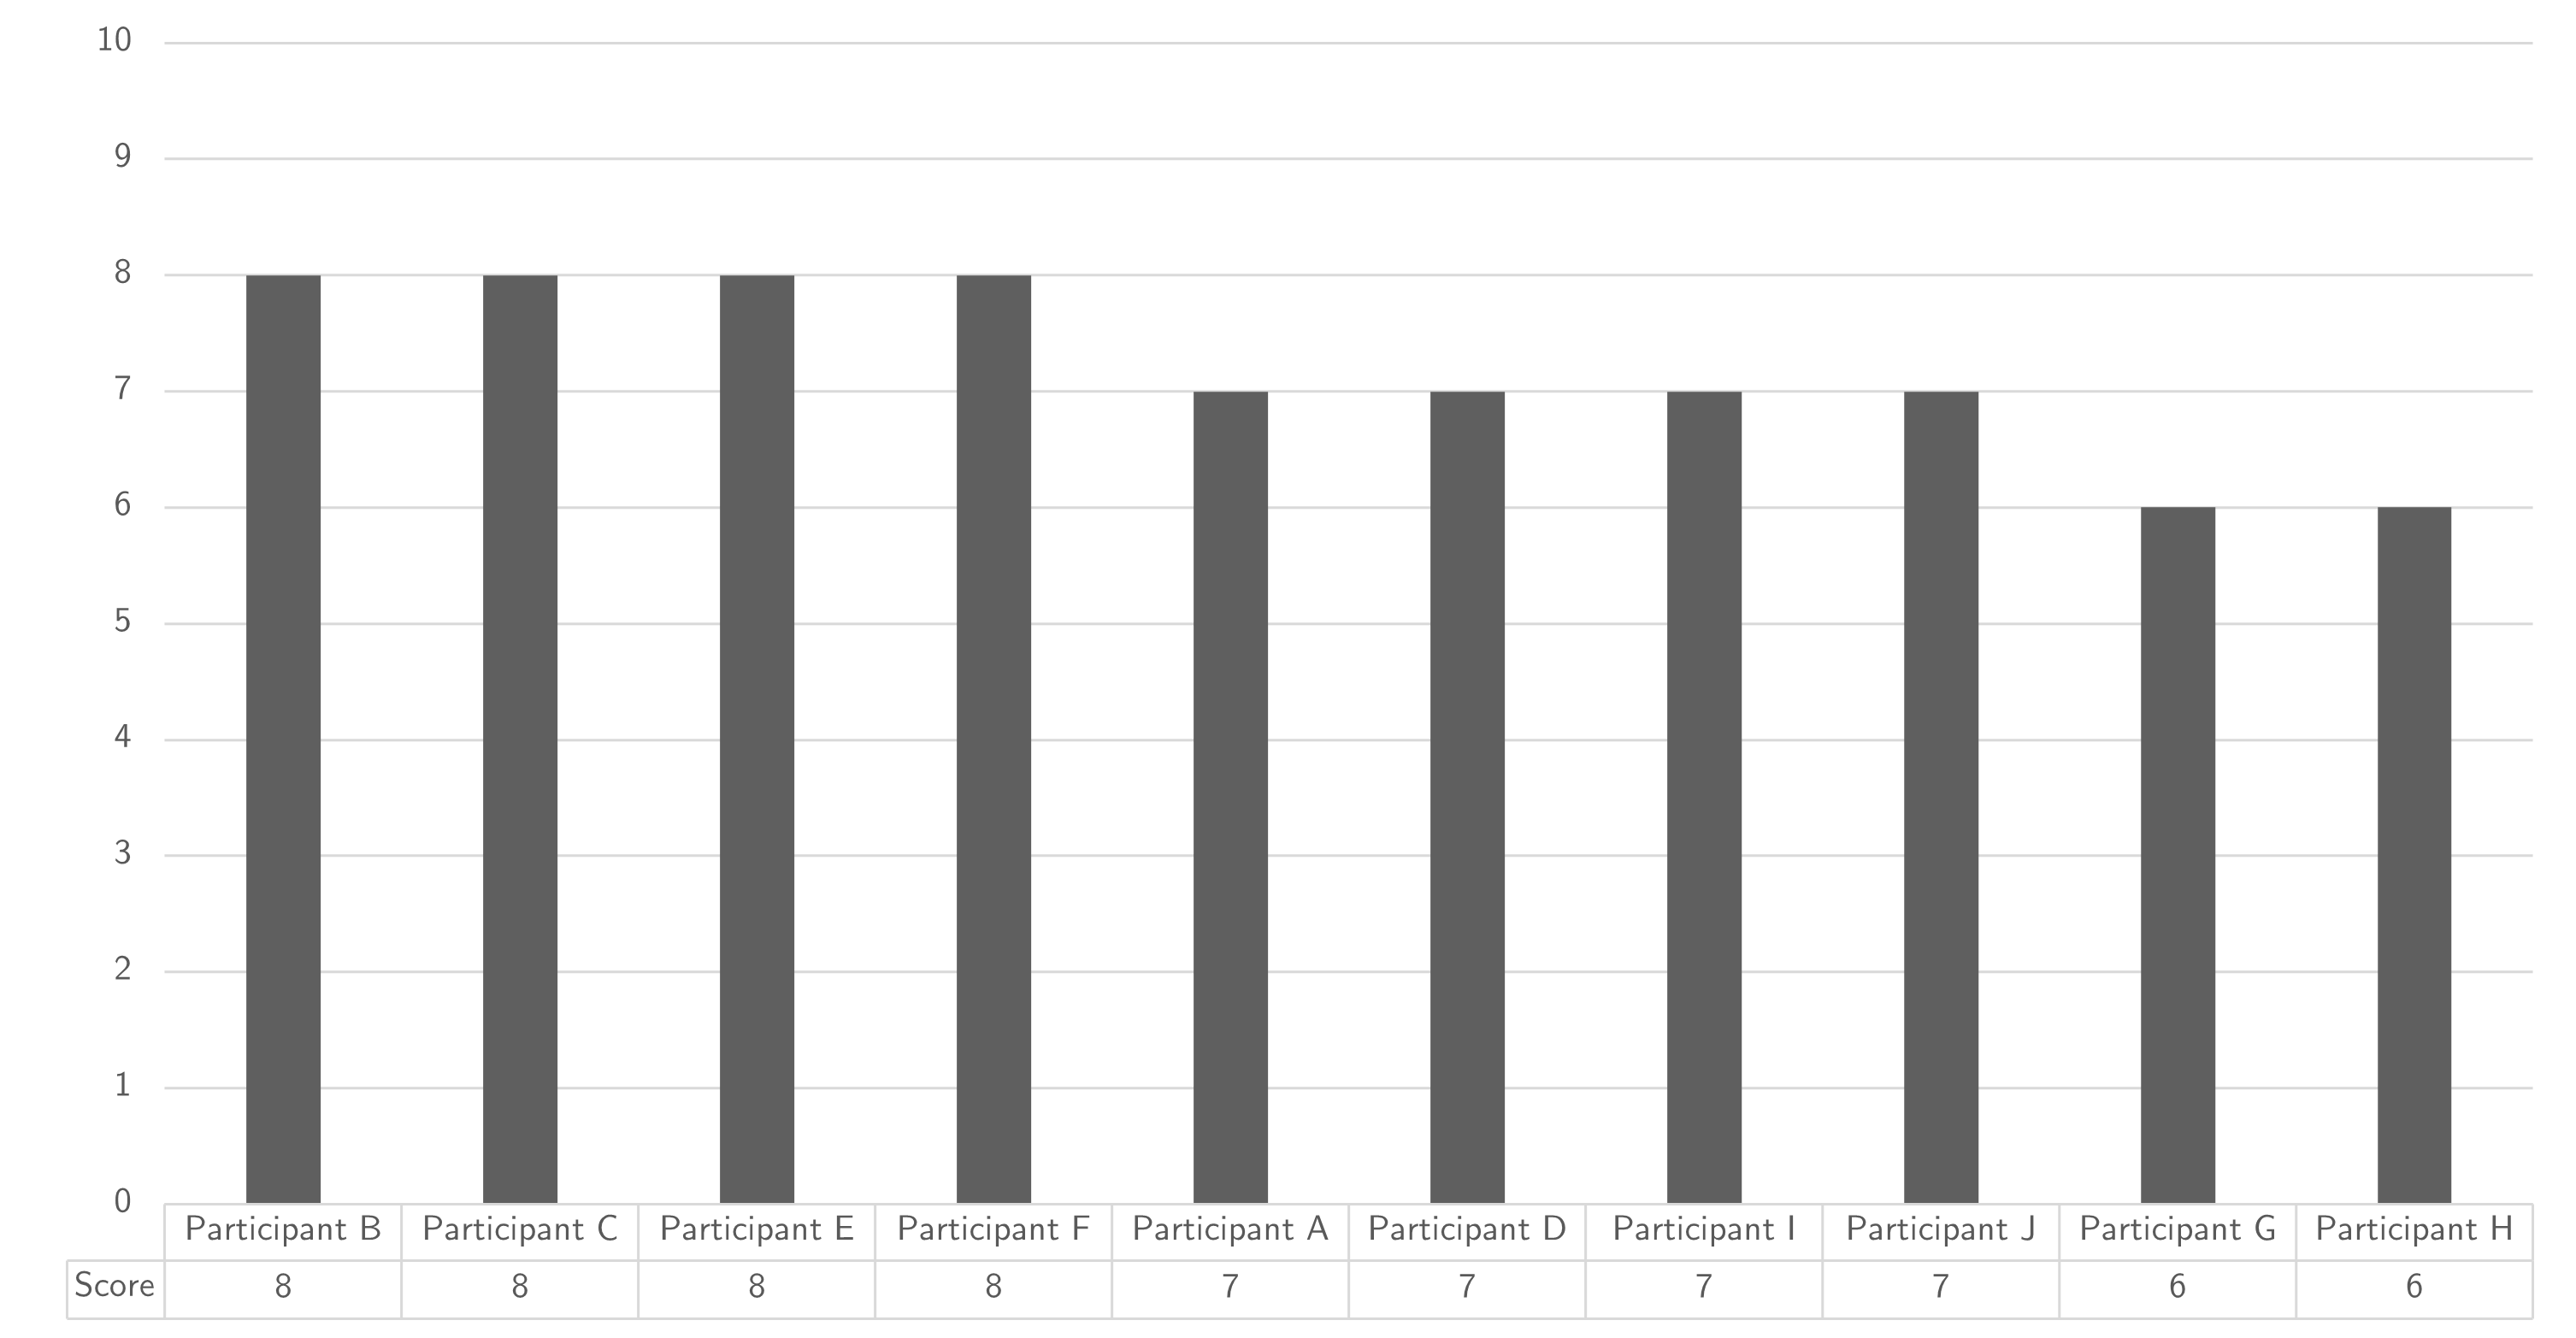
\includegraphics[width=0.9\linewidth]{images/scoreeaschoolenterpriseintegrating}
	\caption[Scoring of school of thought Enterprise Integrating]{Scoring of school of thought Enterprise Integrating}
	\label{fig:appscoringschoolenterpriseintegrating}
\end{figure}
\begin{table}[H]
	\centering
	\begin{tabular}{p{.55\textwidth}ccc}
		\toprule
		\textbf{Attribute} & \textbf{Rating} & \textbf{Variability} & \textbf{Abstains} \\
		\midrule
		Enterprise Integrating & 7,2 & 16\% & 0 \\%
		\bottomrule
	\end{tabular}%
	\caption[Scoring of school of thought Enterprise Integrating]{Scoring of school of thought Enterprise Integrating}
	\label{tab:appscoringschoolenterpriseintegrating}%
\end{table}%
\newpage
\subsection{Enterprise Ecological Adaptation}
\begin{figure}[H]
	\centering
	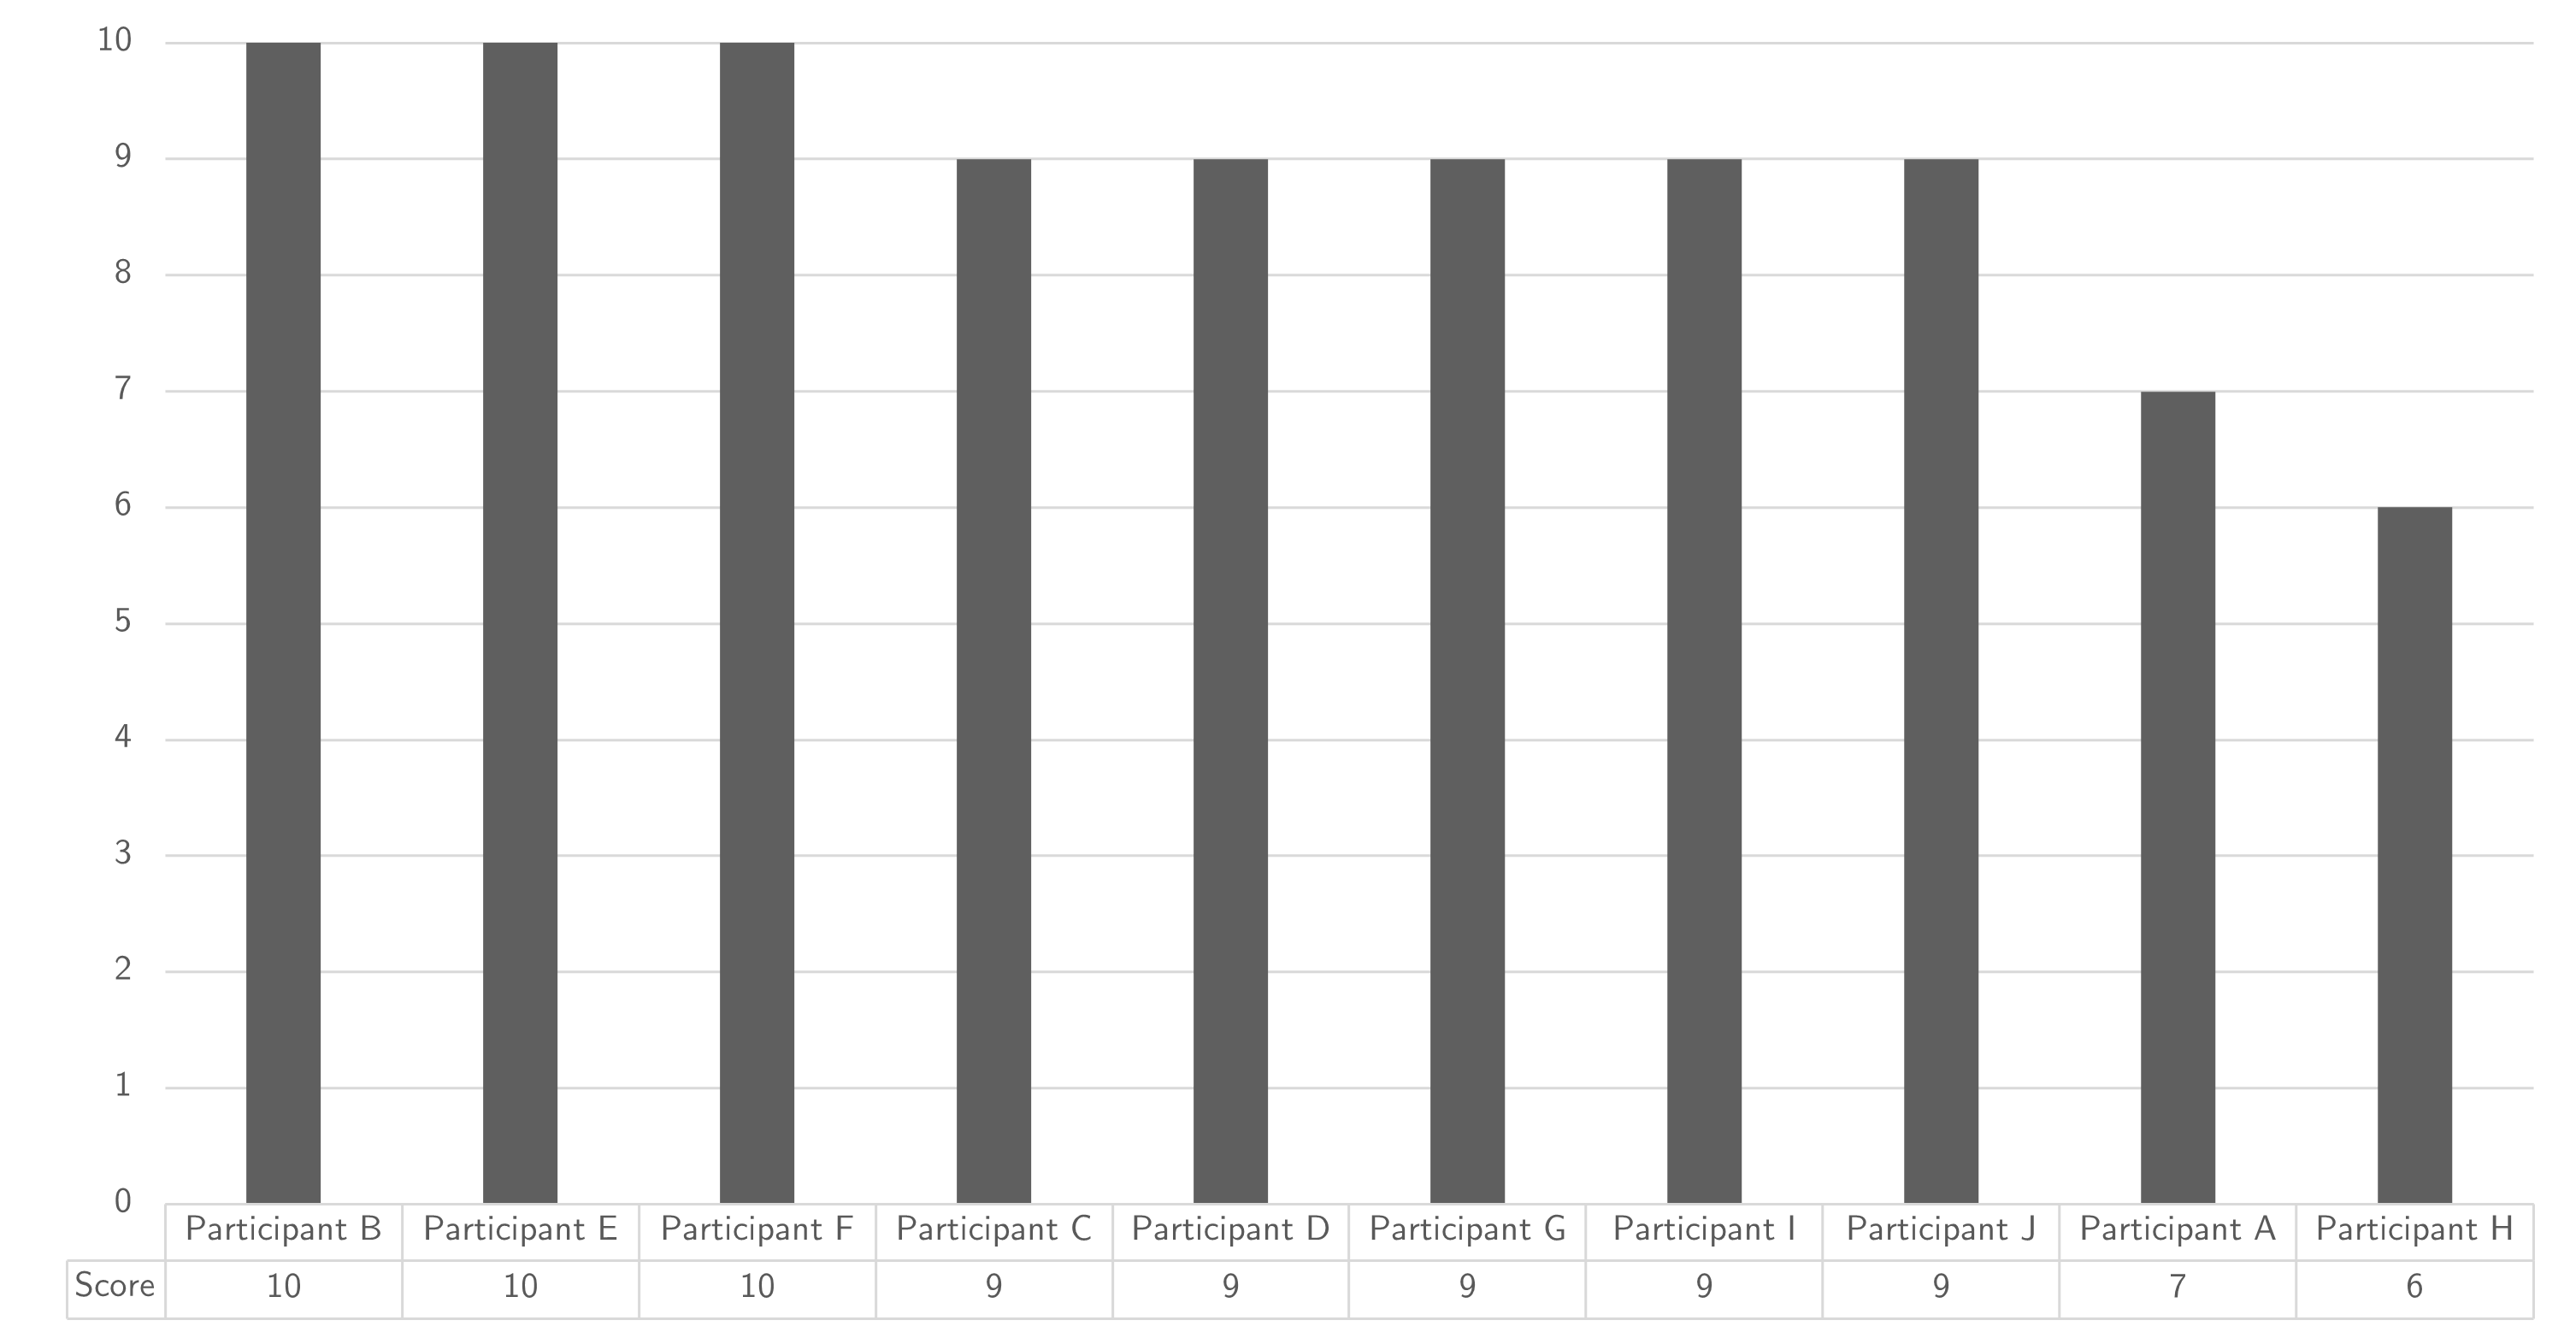
\includegraphics[width=0.9\linewidth]{images/scoreeaschoolenterpriseecologicaladaptation}
	\caption[Scoring of school of thought Enterprise Ecological Adaptation]{Scoring of school of thought Enterprise Ecological Adaptation}
	\label{fig:appscoringschoolenterpriseecologicaladaptation}
\end{figure}
\begin{table}[H]
	\centering
	\begin{tabular}{p{.55\textwidth}ccc}
		\toprule
		\textbf{Attribute} & \textbf{Rating} & \textbf{Variability} & \textbf{Abstains} \\
		\midrule
		Enterprise Ecological Adaptation & 8,8 & 27\% & 0 \\%
		\bottomrule
	\end{tabular}%
	\caption[Scoring of school of thought Enterprise Ecological Adaptation]{Scoring of school of thought Enterprise Ecological Adaptation}
	\label{tab:appscoringschoolenterpriseecologicaladaptation}%
\end{table}%

\newpage
\section{Validation of Enterprise Architecture attributes}
\label{sec:validationofeaattributes}
\begin{table}[H]
	\centering
	\begin{tabular}{p{.55\textwidth}ccc}
		\toprule
		\textbf{Attribute} & \textbf{Rating} & \textbf{Variability} & \textbf{Abstains} \\
		\midrule
		Systems-in-environment thinking & 7,7 & 28\% & 0 \\%
		Holist (systemic) stance & 7 & 47\% & 0 \\%
		Organisational learning & 7,3 & 44\% & 0 \\%
		Environmental learning & 7,7 & 29\% & 0 \\%
		Intra-organisational coherency & 6,4 & 31\% & 0 \\%
		System-in-environment coevolution learning & 6,6 & 36\% & 0 \\%
		Adapt to business language & 7,1 & 35\% & 0 \\%
		Agile Enterprise & 6,4 & 50\% & 0 \\%
		Real Time Trust (Policy \& Attribute based) & 5,6 & 54\% & 1 \\%
		Foster Dialogue & 6,9 & 32\% & 0 \\%
		Validation & 7,4 & 24\% & 0 \\%
		Altijd goed architectuur & 5,8 & 46\% & 1 \\%
		\bottomrule
	\end{tabular}%
	\caption{Validation of Enterprise Architecture attributes}
	\label{tab:appvalidationofeaattributes}%
\end{table}%
\newpage
\subsection{Systems-in-Environment thinking}
\begin{figure}[H]
	\centering
	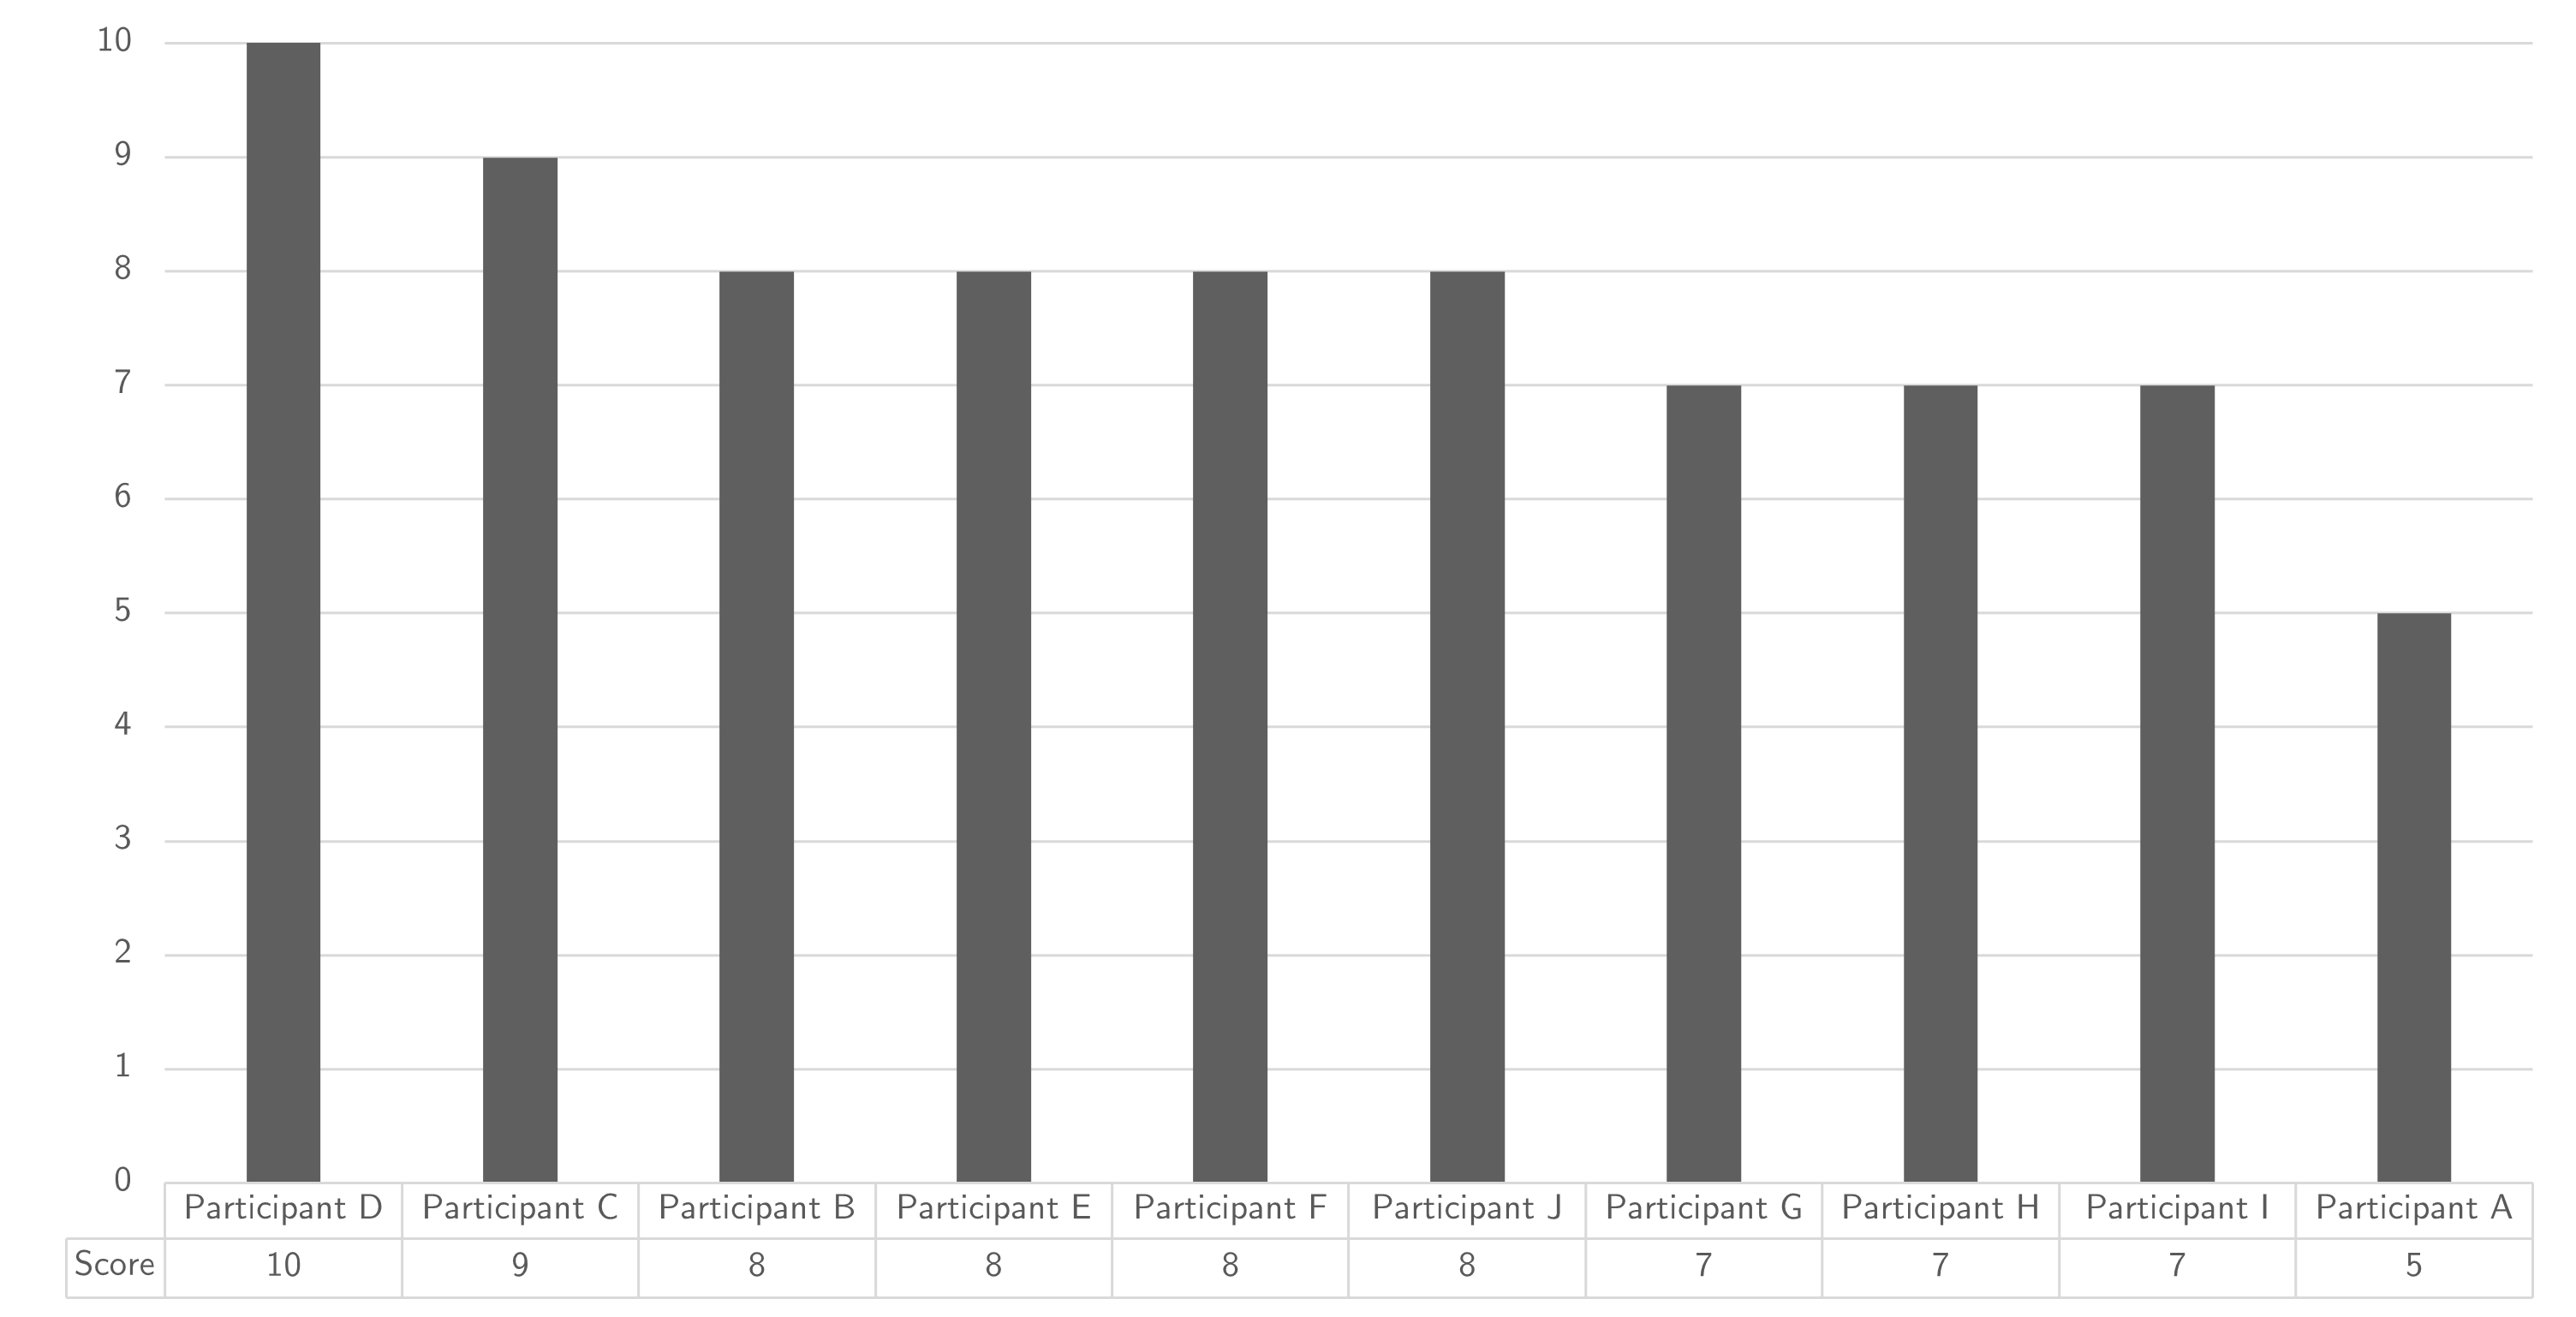
\includegraphics[width=0.9\linewidth]{images/scoreeasystemsinenvironmentthinking}
	\caption[Scoring of EA attribute Systems-in-Environment thinking]{Scoring of EA attribute Systems-in-Environment thinking}
	\label{fig:appscoringeasystemsinenvironmentthinking}
\end{figure}
\begin{table}[H]
	\centering
	\begin{tabular}{p{.55\textwidth}ccc}
		\toprule
		\textbf{Attribute} & \textbf{Rating} & \textbf{Variability} & \textbf{Abstains} \\
		\midrule
		Systems-in-environment thinking & 7,7 & 28\% & 0 \\%
		\bottomrule
	\end{tabular}%
	\caption[Scoring of EA attribute Systems-in-Environment thinking]{Scoring of EA attribute Systems-in-Environment thinking}
	\label{tab:appscoringeasystemsinenvironmentthinking}%
\end{table}%
\newpage
\subsection{Holistic (systemic) stance}
\begin{figure}[H]
	\centering
	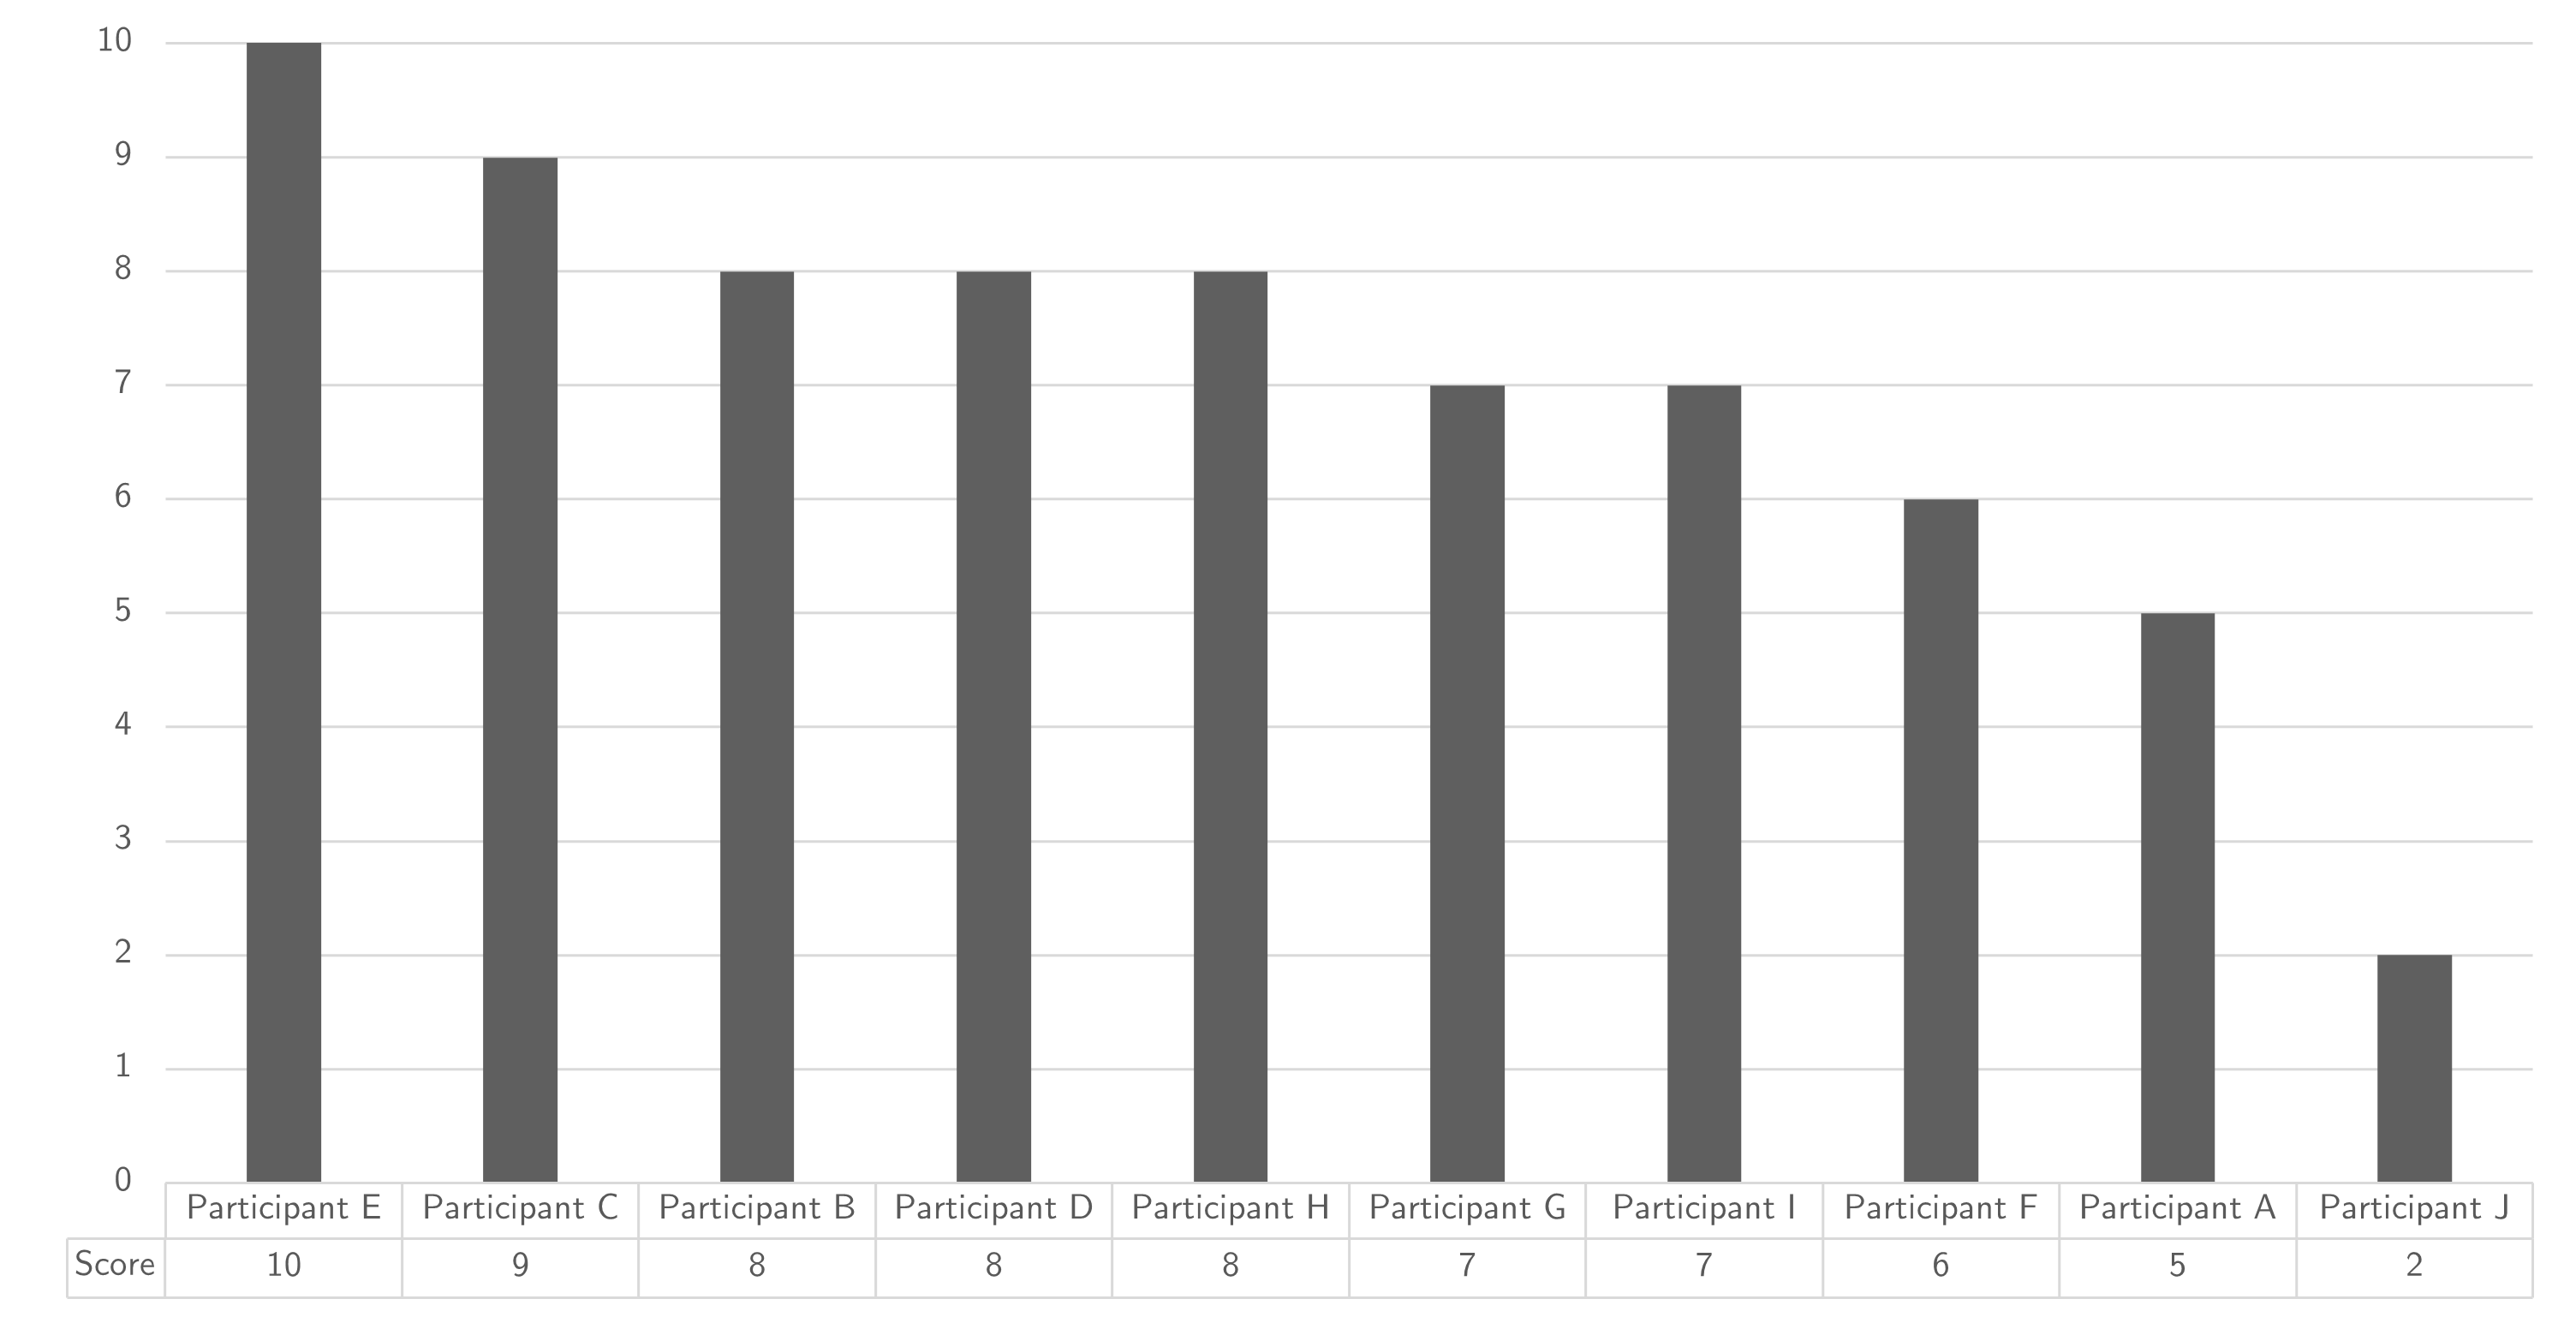
\includegraphics[width=0.9\linewidth]{images/scoreeaholisticsystemsstance}
	\caption[Scoring of EA attribute Holistic (systemic) stance]{Scoring of EA attribute Holistic (systemic) stance}
	\label{fig:appscoringeaholisticsystemsstance}
\end{figure}
\begin{table}[H]
	\centering
	\begin{tabular}{p{.55\textwidth}ccc}
		\toprule
		\textbf{Attribute} & \textbf{Rating} & \textbf{Variability} & \textbf{Abstains} \\
		\midrule
		Holist (systemic) stance & 7 & 47\% & 0 \\%
		\bottomrule
	\end{tabular}%
	\caption[Scoring of EA attribute Holistic (systemic) stance]{Scoring of EA attribute Holistic (systemic) stance}
	\label{tab:appscoringeaholisticsystemsstance}%
\end{table}%
\newpage
\subsection{Organisational learning}
\begin{figure}[H]
	\centering
	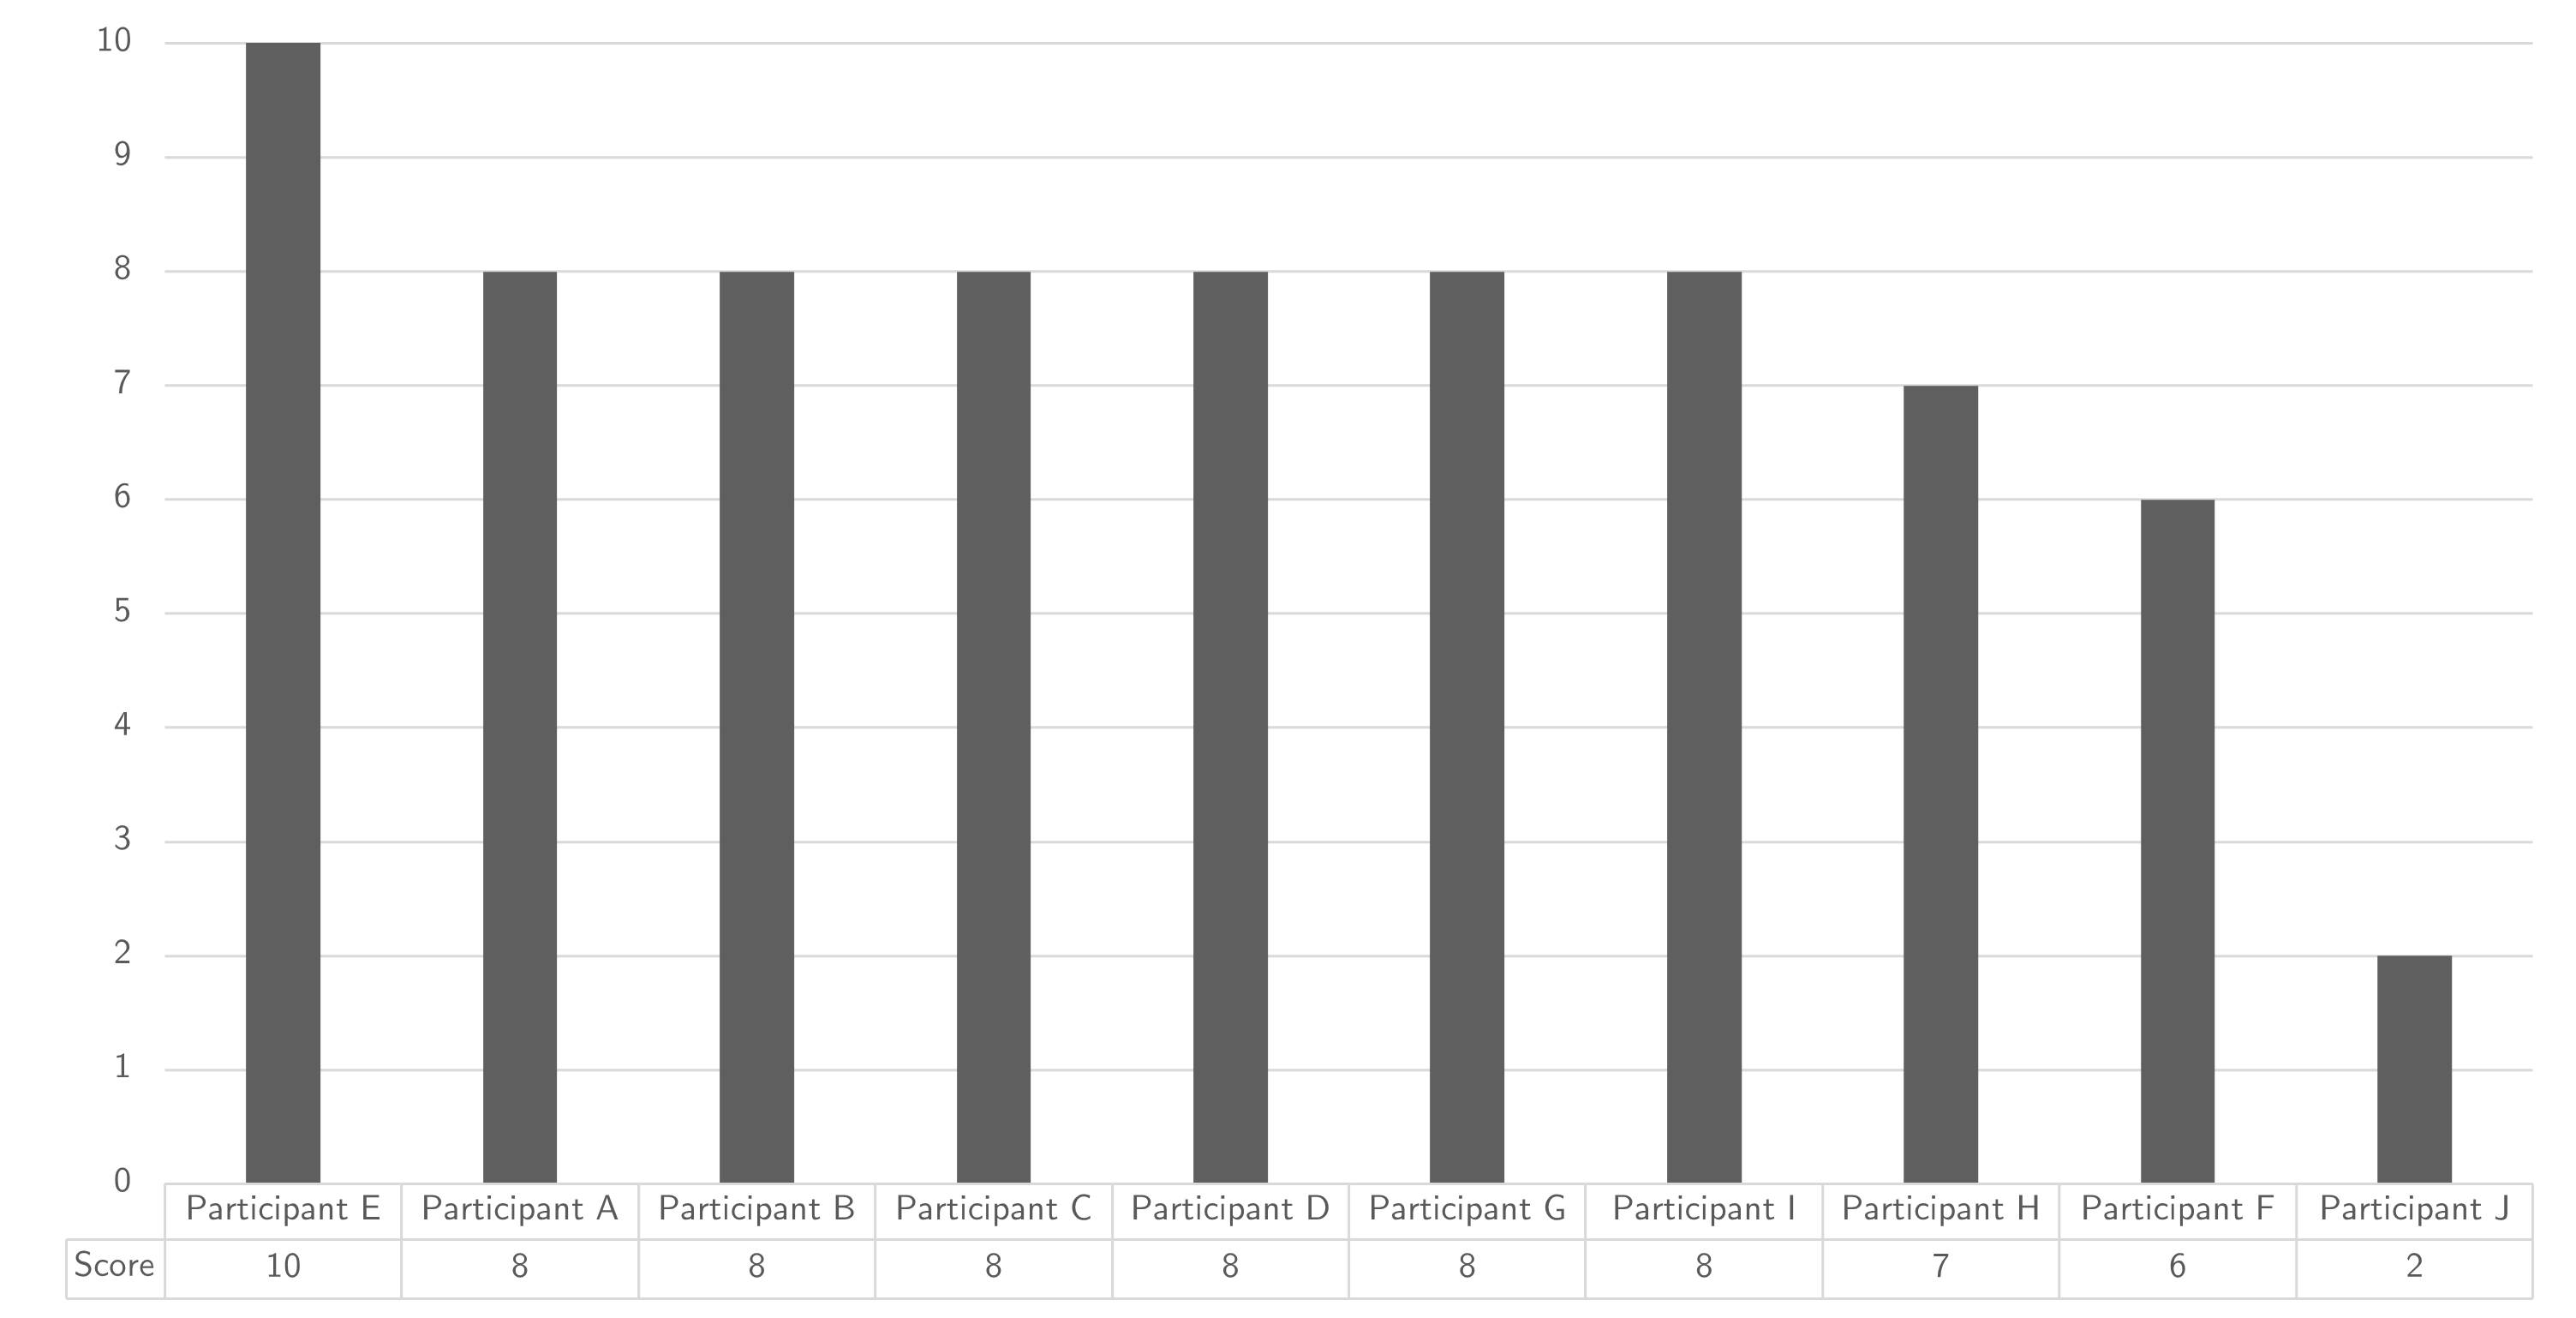
\includegraphics[width=0.9\linewidth]{images/scoreeaorganisationallearning}
	\caption[Scoring of EA attribute Organisational learning]{Scoring of EA attribute Organisational learning}
	\label{fig:appscoringeaorganiationallearning}
\end{figure}
\begin{table}[H]
	\centering
	\begin{tabular}{p{.55\textwidth}ccc}
		\toprule
		\textbf{Attribute} & \textbf{Rating} & \textbf{Variability} & \textbf{Abstains} \\
		\midrule
		Organisational learning & 7,3 & 44\% & 0 \\%
		\bottomrule
	\end{tabular}%
	\caption[Scoring of EA attribute Organisational learning]{Scoring of EA attribute Organisational learning}
	\label{tab:appscoringeaorganisationallearning}%
\end{table}%
\newpage
\subsection{Environmental learning}
\begin{figure}[H]
	\centering
	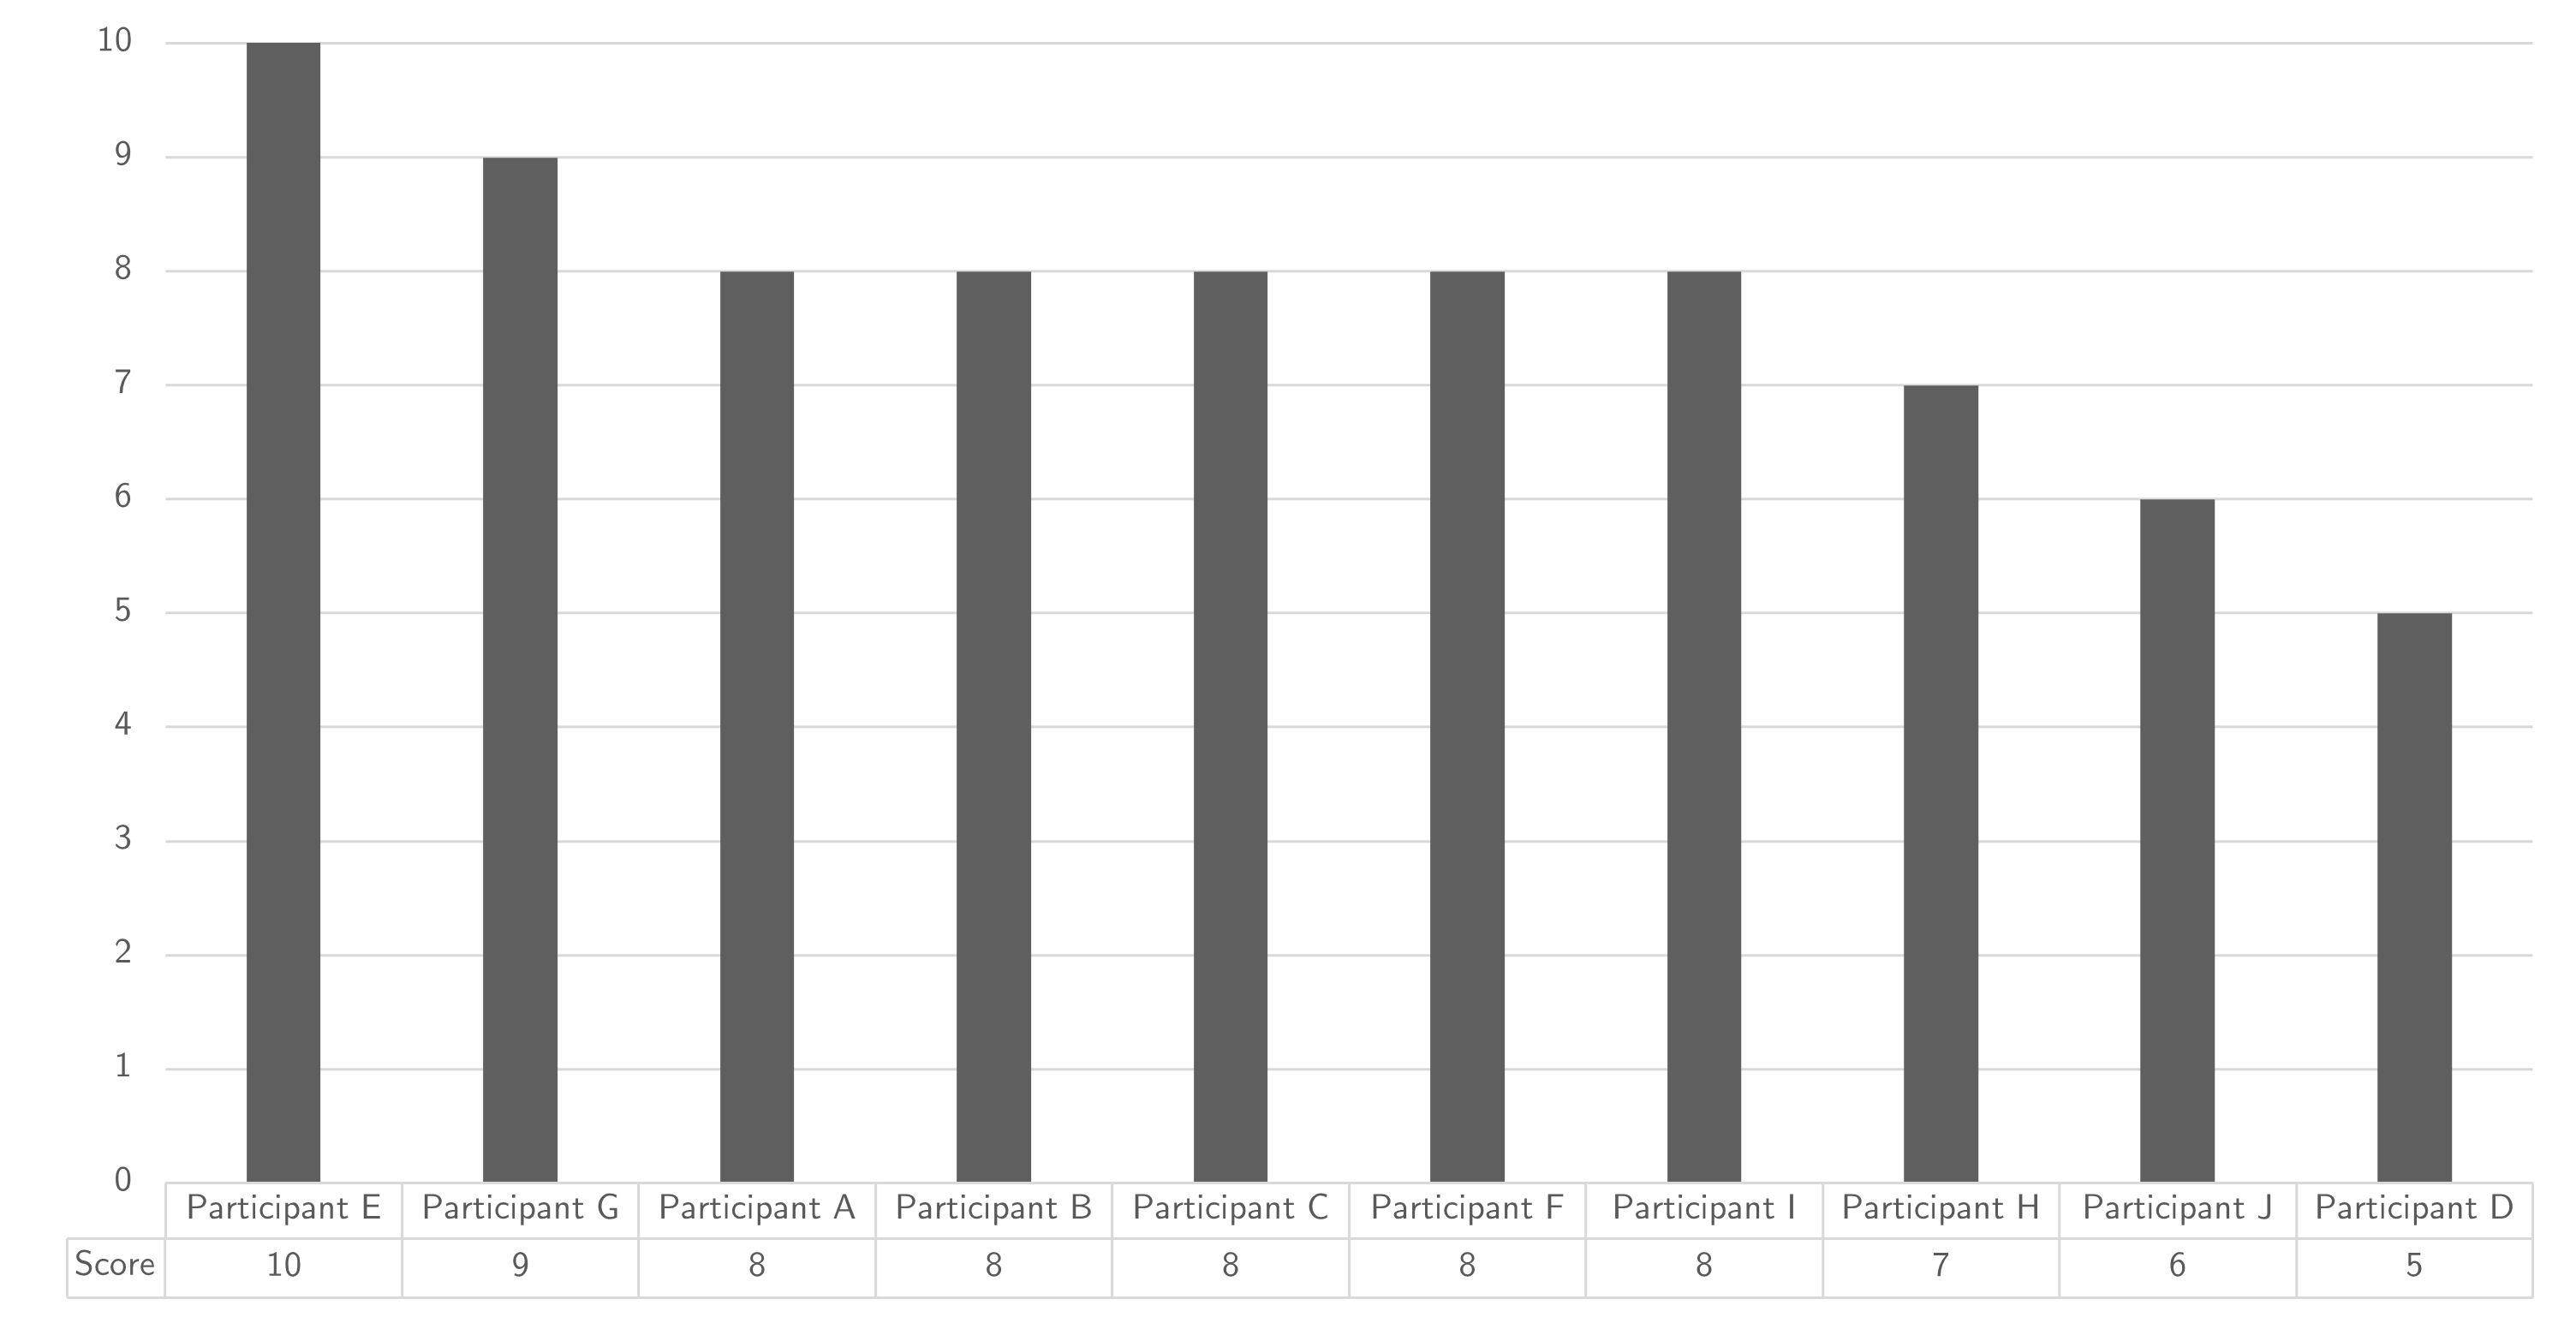
\includegraphics[width=0.9\linewidth]{images/scoreeaenvironmentallearning}
	\caption[Scoring of EA attribute Environmental learning]{Scoring of EA attribute Environmental learning}
	\label{fig:appscoringeaenvironmentallearning}
\end{figure}
\begin{table}[H]
	\centering
	\begin{tabular}{p{.55\textwidth}ccc}
		\toprule
		\textbf{Attribute} & \textbf{Rating} & \textbf{Variability} & \textbf{Abstains} \\
		\midrule
		Environmental learning & 7,7 & 29\% & 0 \\%
		\bottomrule
	\end{tabular}%
	\caption[Scoring of EA attribute Environmental learning]{Scoring of EA attribute Environmental learning}
	\label{tab:appscoringeaenvironmentallearning}%
\end{table}%
\newpage
\subsection{Intra-organisational coherency}
\begin{figure}[H]
	\centering
	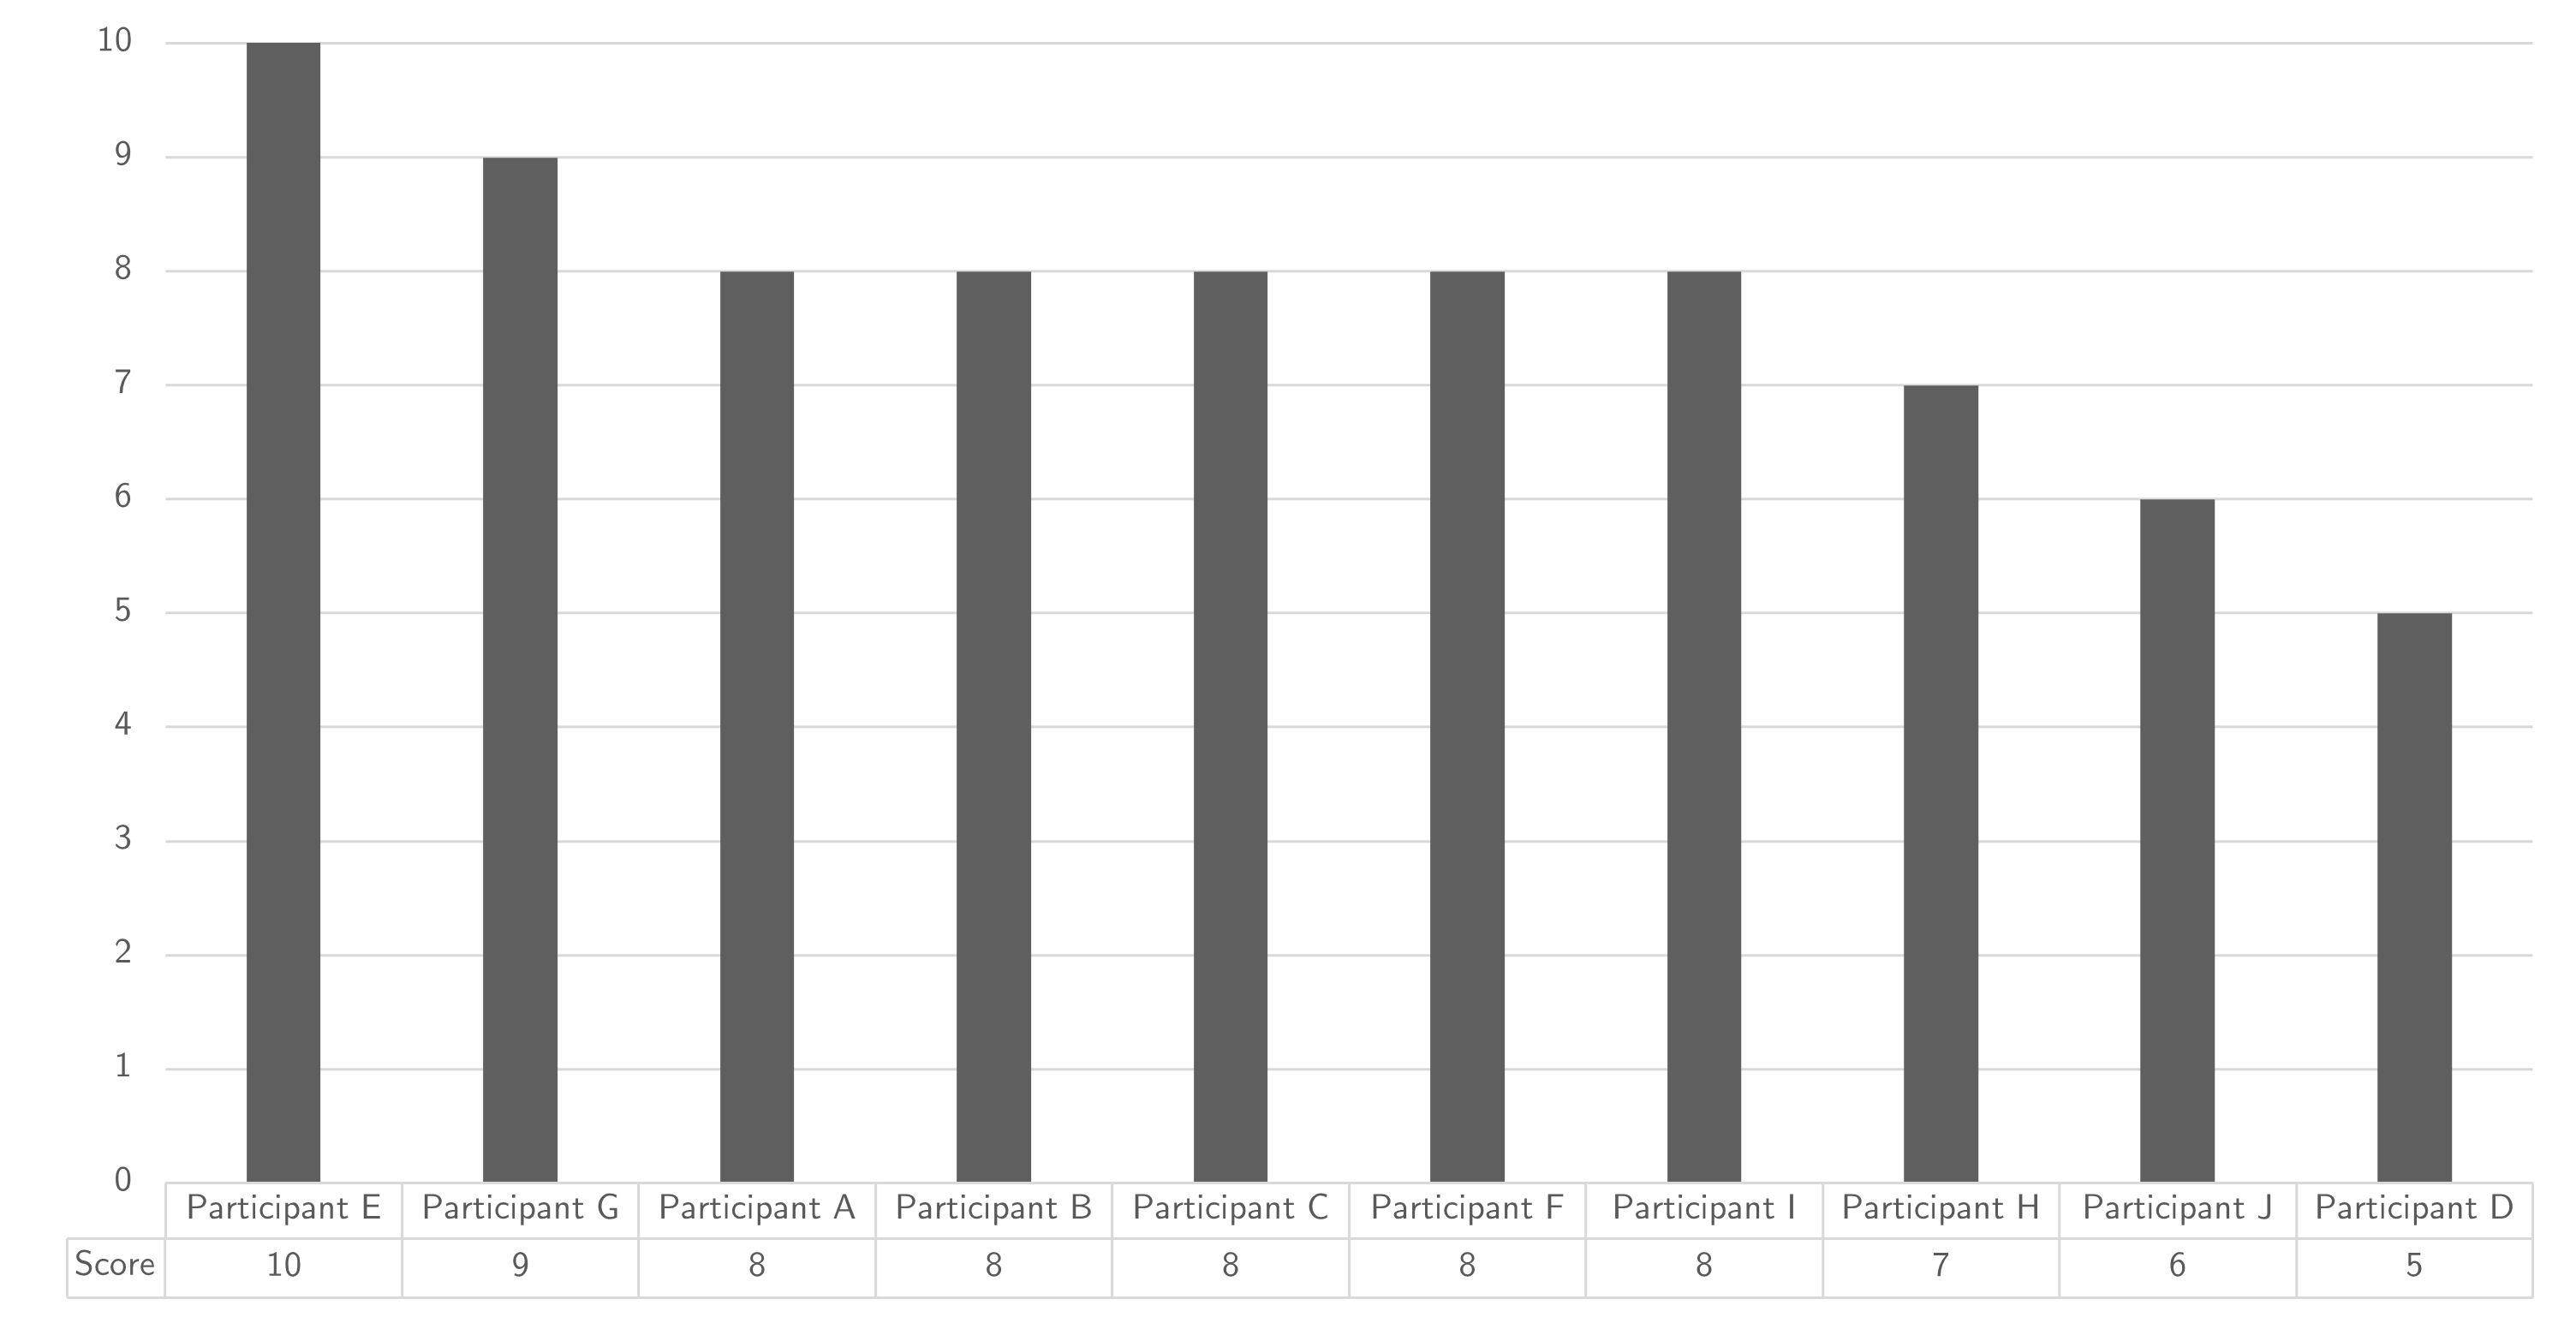
\includegraphics[width=0.9\linewidth]{images/scoreeaintraorganisationalcoherency}
	\caption[Scoring of EA attribute Intra-Organisational coherency]{Scoring of EA attribute Intra-Organisational coherency}
	\label{fig:appscoringeaintraorganisationalcoherency}
\end{figure}
\begin{table}[H]
	\centering
	\begin{tabular}{p{.55\textwidth}ccc}
		\toprule
		\textbf{Attribute} & \textbf{Rating} & \textbf{Variability} & \textbf{Abstains} \\
		\midrule
		Intra-organisational coherency & 6,4 & 31\% & 0 \\%
		\bottomrule
	\end{tabular}%
	\caption[Scoring of EA attribute Intra-Organisational coherency]{Scoring of EA attribute Intra-Organisational coherency}
	\label{tab:appscoringeaintraorganisationalcoherency}%
\end{table}%
\newpage
\subsection{System-in-Environment Co-Evolution learning}
\begin{figure}[H]
	\centering
	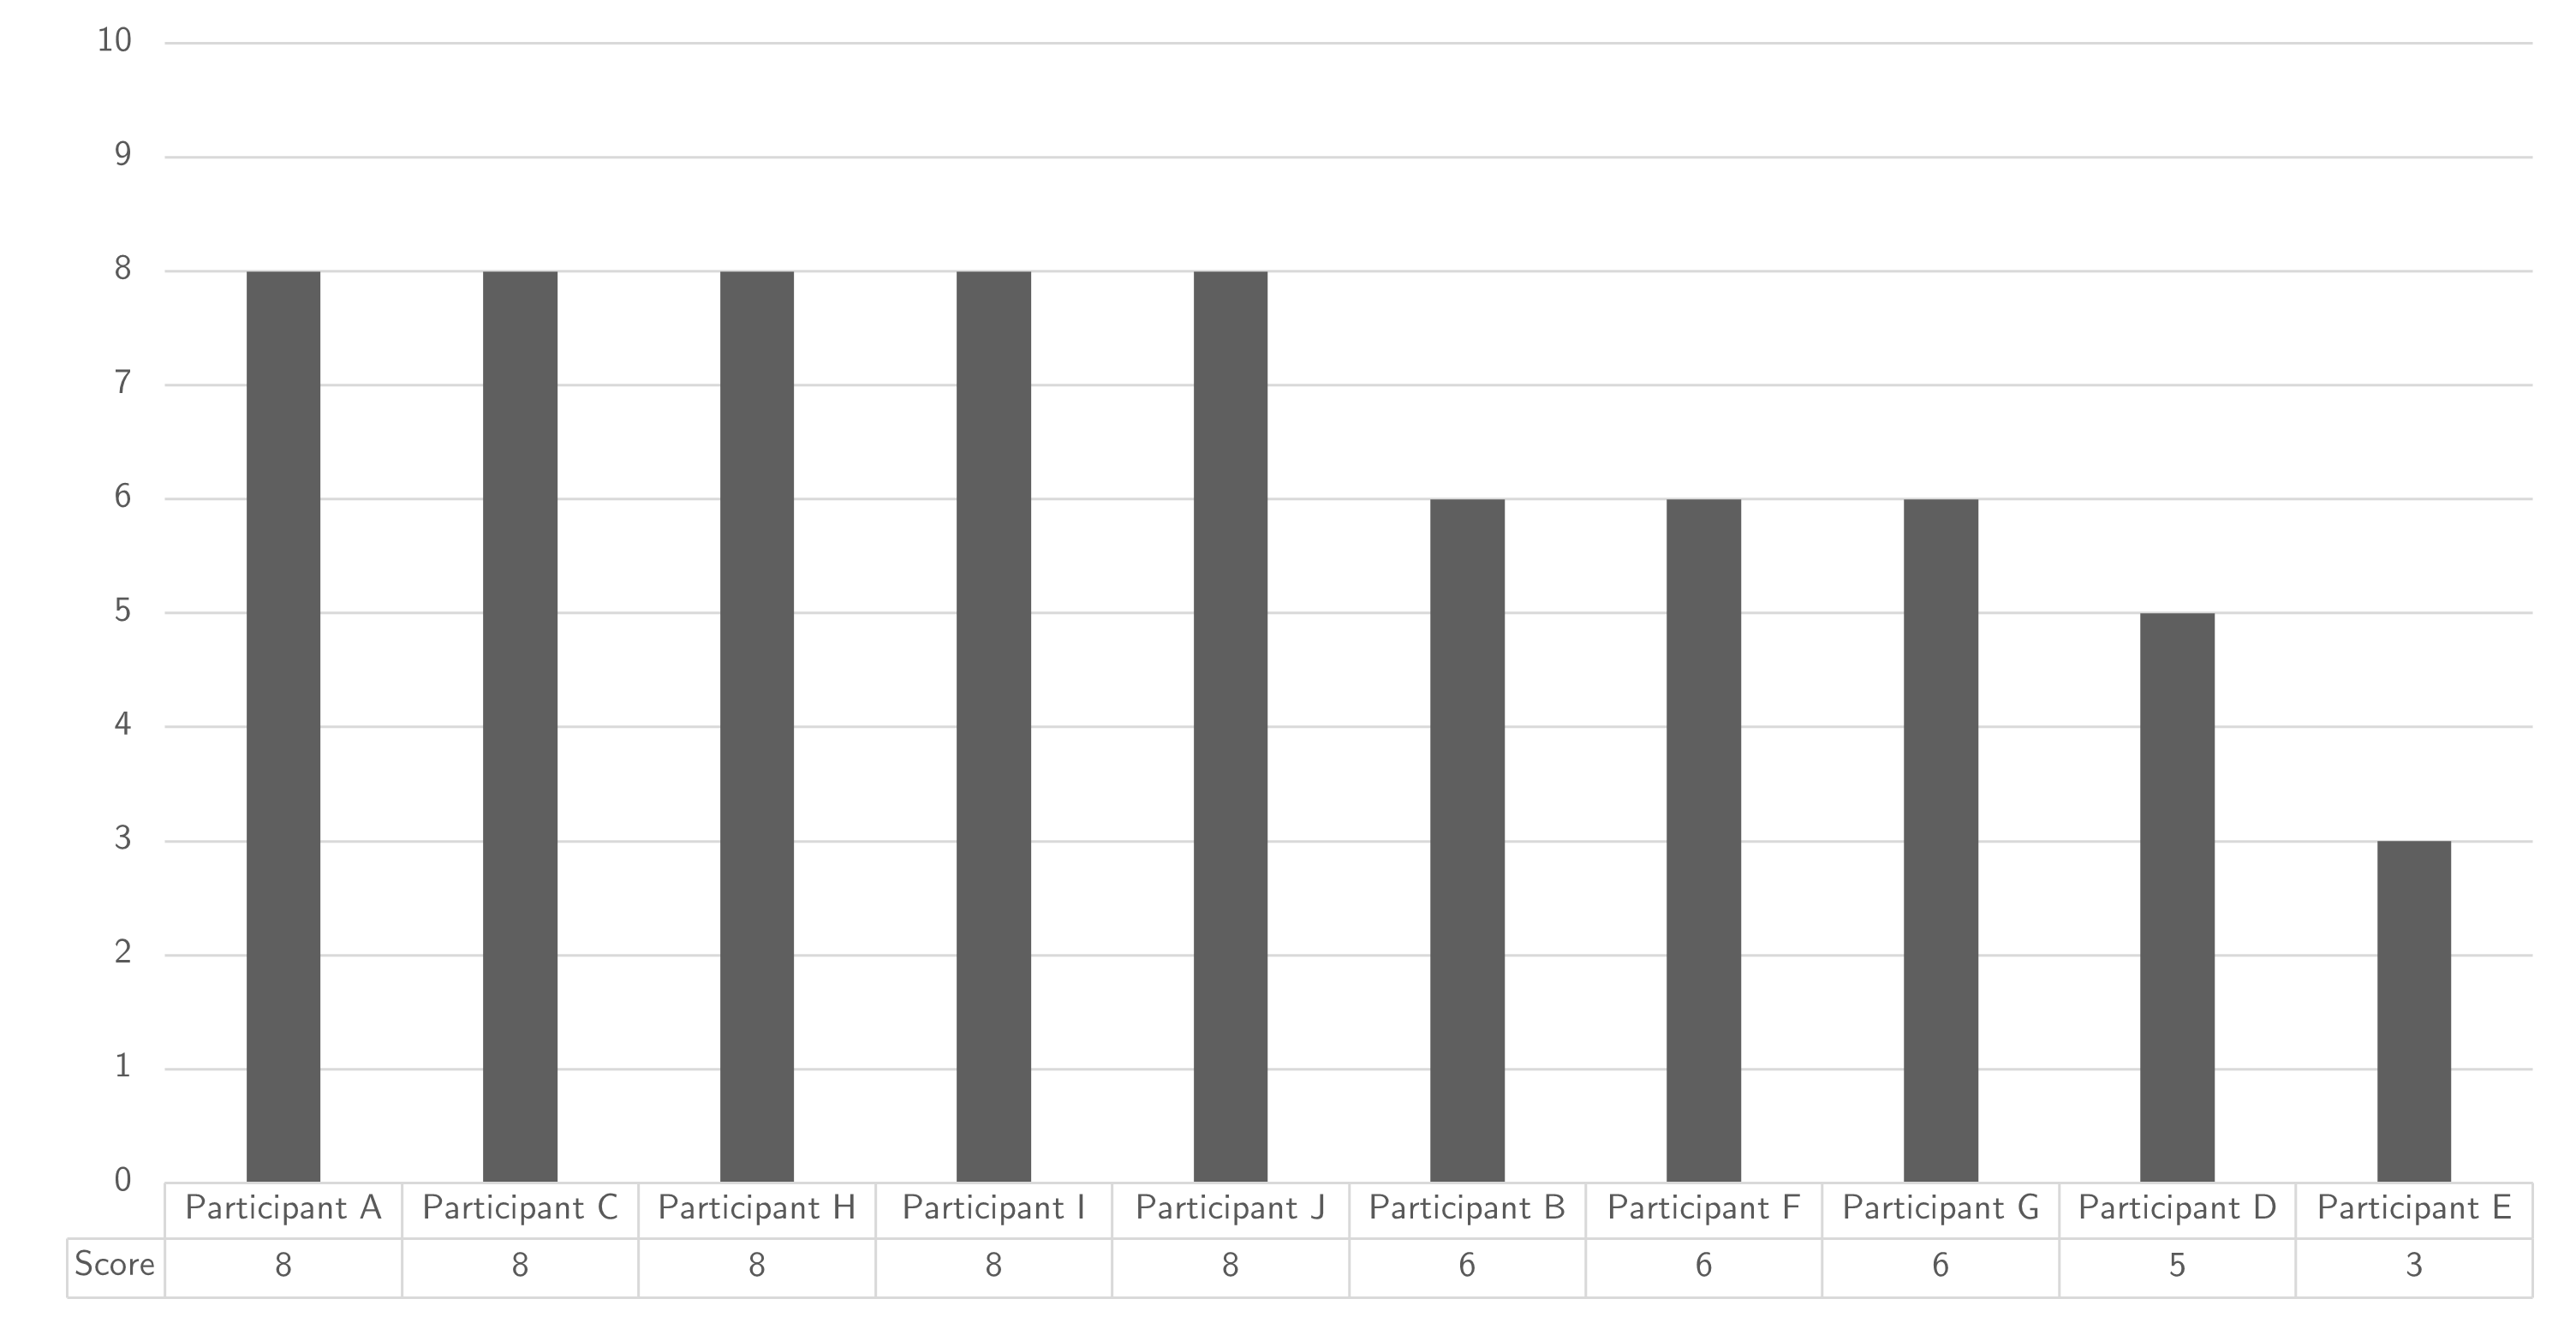
\includegraphics[width=0.9\linewidth]{images/scoreeasysteminenvironmentcoevolution}
	\caption[Scoring of EA attribute System-in-Environment Co-Evolution learning]{Scoring of EA attribute System-in-Environment Co-Evolution learning}
	\label{fig:appscoringeasysteminenvironmentcoevolutionlearning}
\end{figure}
\begin{table}[H]
	\centering
	\begin{tabular}{p{.55\textwidth}ccc}
		\toprule
		\textbf{Attribute} & \textbf{Rating} & \textbf{Variability} & \textbf{Abstains} \\
		\midrule
		System-in-environment coevolution learning & 6,6 & 36\% & 0 \\%
		\bottomrule
	\end{tabular}%
	\caption[Scoring of EA attribute System-in-Environment Co-Evolution learning]{Scoring of EA attribute System-in-Environment Co-Evolution learning}
	\label{tab:appscoringeasysteminenvironmentcoevolutionlearning}%
\end{table}%
\newpage
\subsection{Adapt to business language}
\begin{figure}[H]
	\centering
	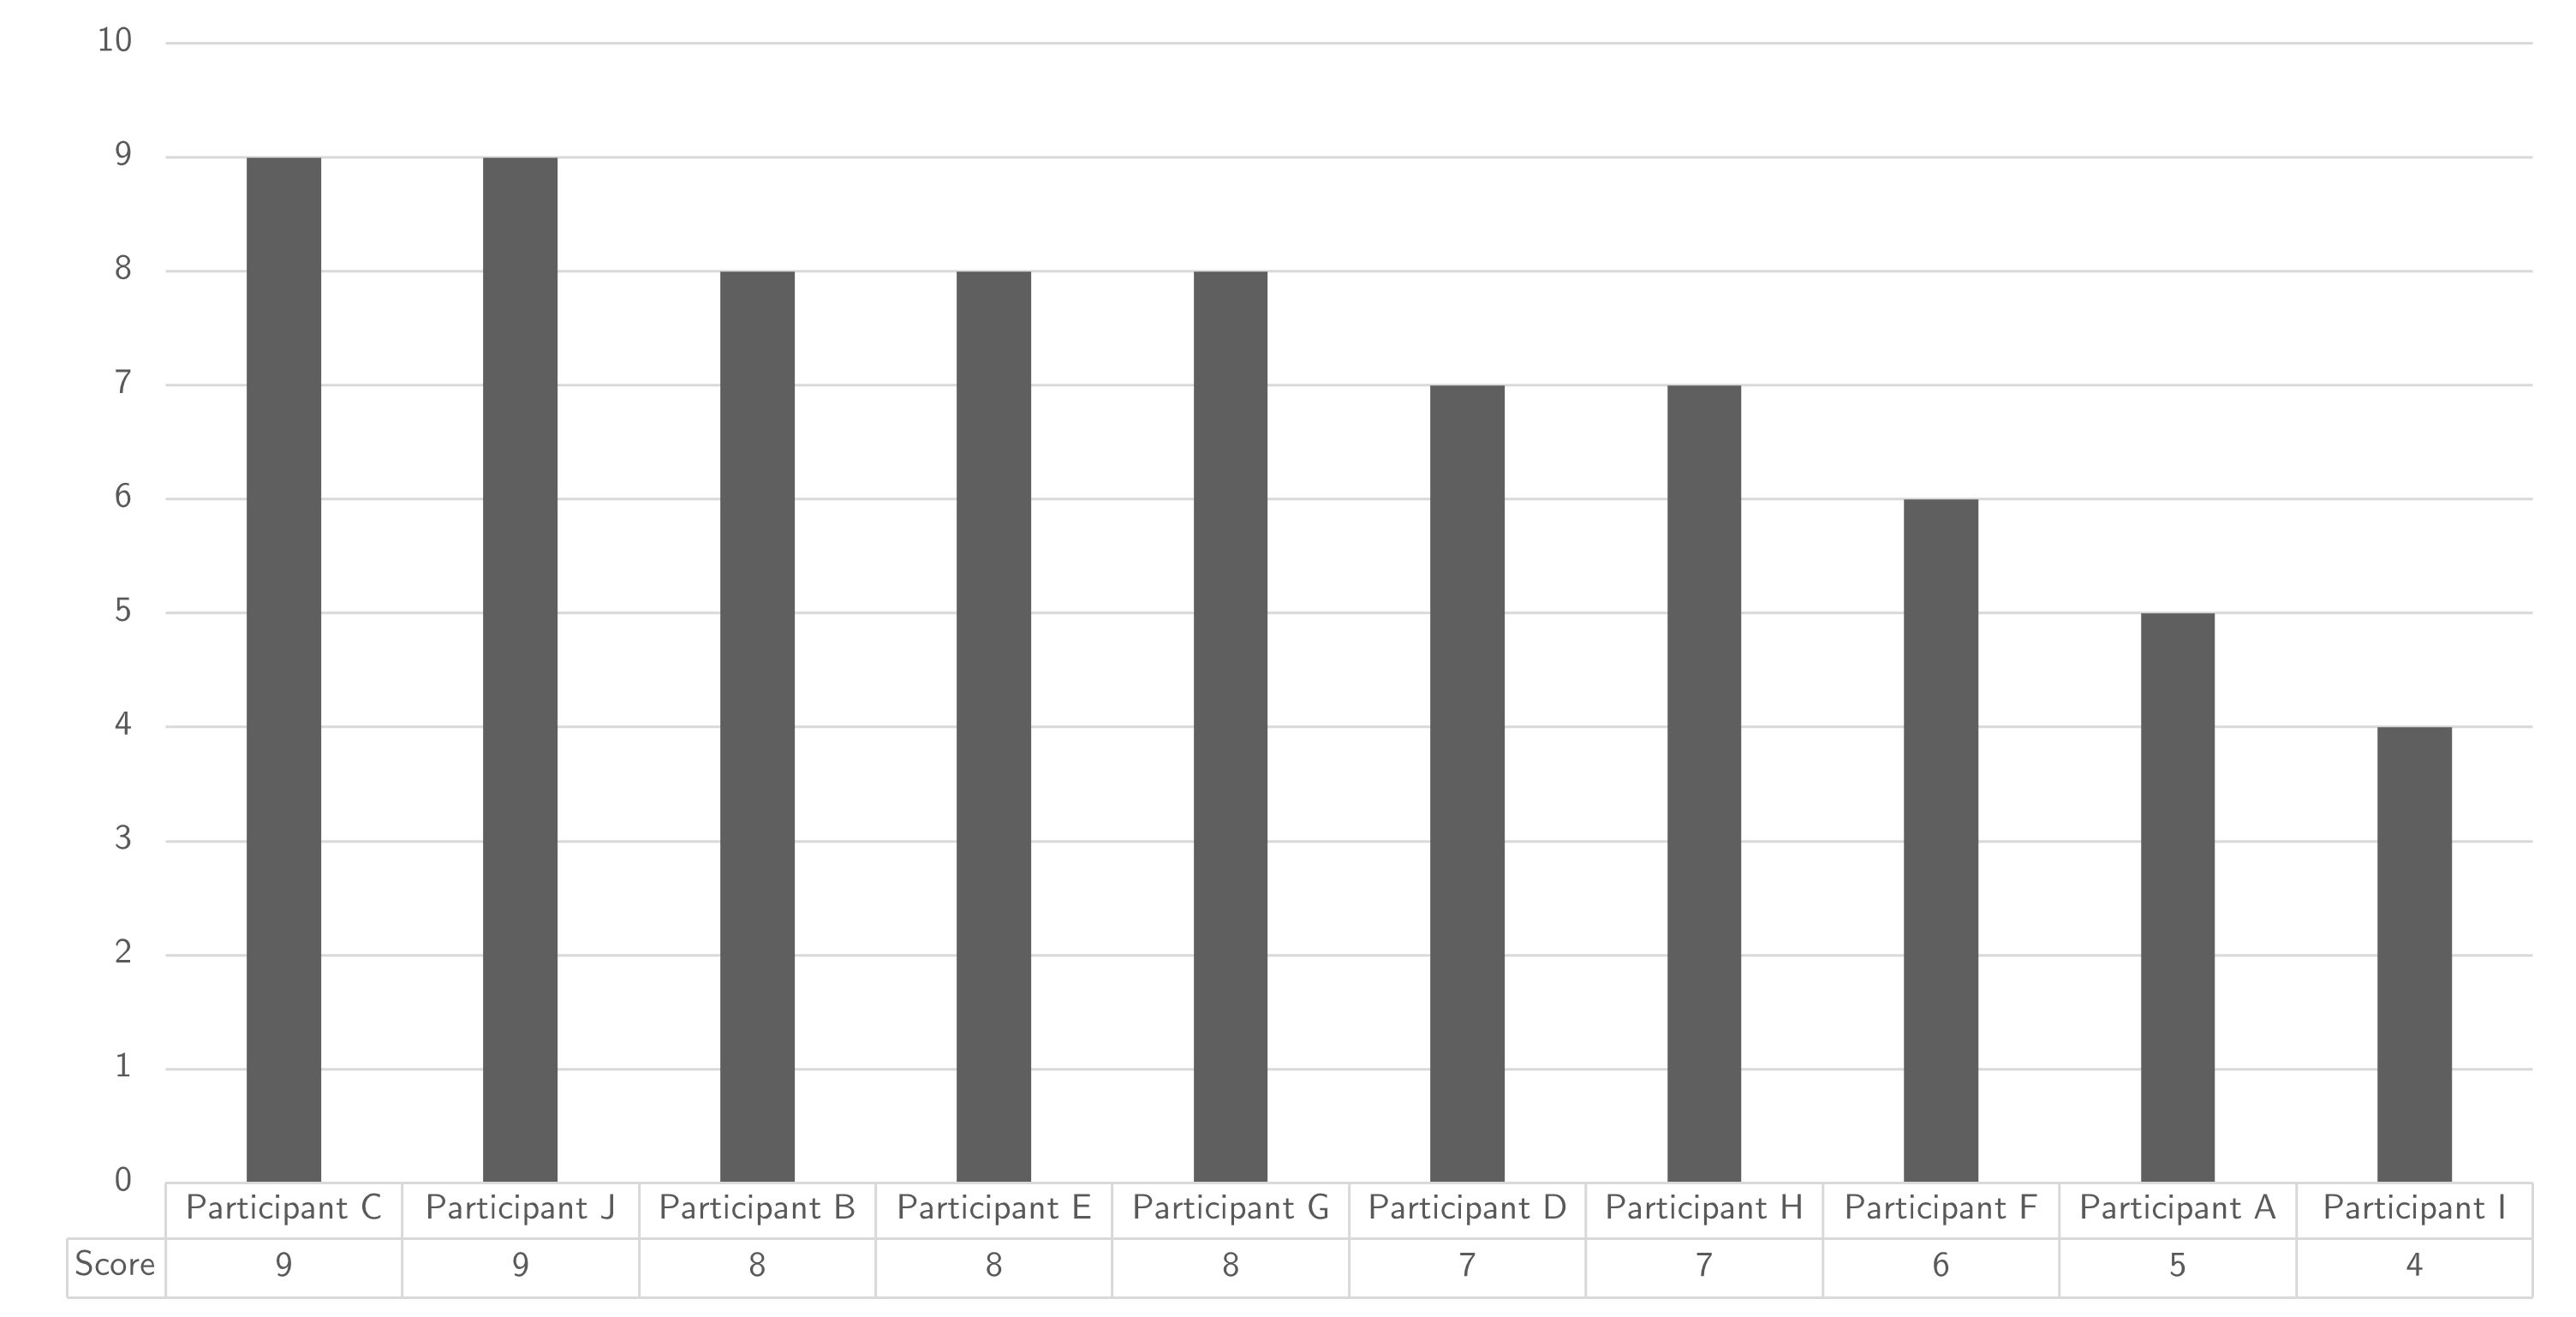
\includegraphics[width=0.9\linewidth]{images/scoreeaadapttobusinesslanguage}
	\caption[Scoring of EA attribute adapt to business language]{Scoring of EA attribute adapt to business language}
	\label{fig:appscoringeaadapttobusinesslanguage}
\end{figure}
\begin{table}[H]
	\centering
	\begin{tabular}{p{.55\textwidth}ccc}
		\toprule
		\textbf{Attribute} & \textbf{Rating} & \textbf{Variability} & \textbf{Abstains} \\
		\midrule
		Adapt to business language & 7,1 & 35\% & 0 \\%
		\bottomrule
	\end{tabular}%
	\caption[Scoring of EA attribute adapt to business language]{Scoring of EA attribute adapt to business language}
	\label{tab:appscoringeaadapttobusinesslanguage}%
\end{table}%
\newpage
\subsection{Agile Enterprise}
\begin{figure}[H]
	\centering
	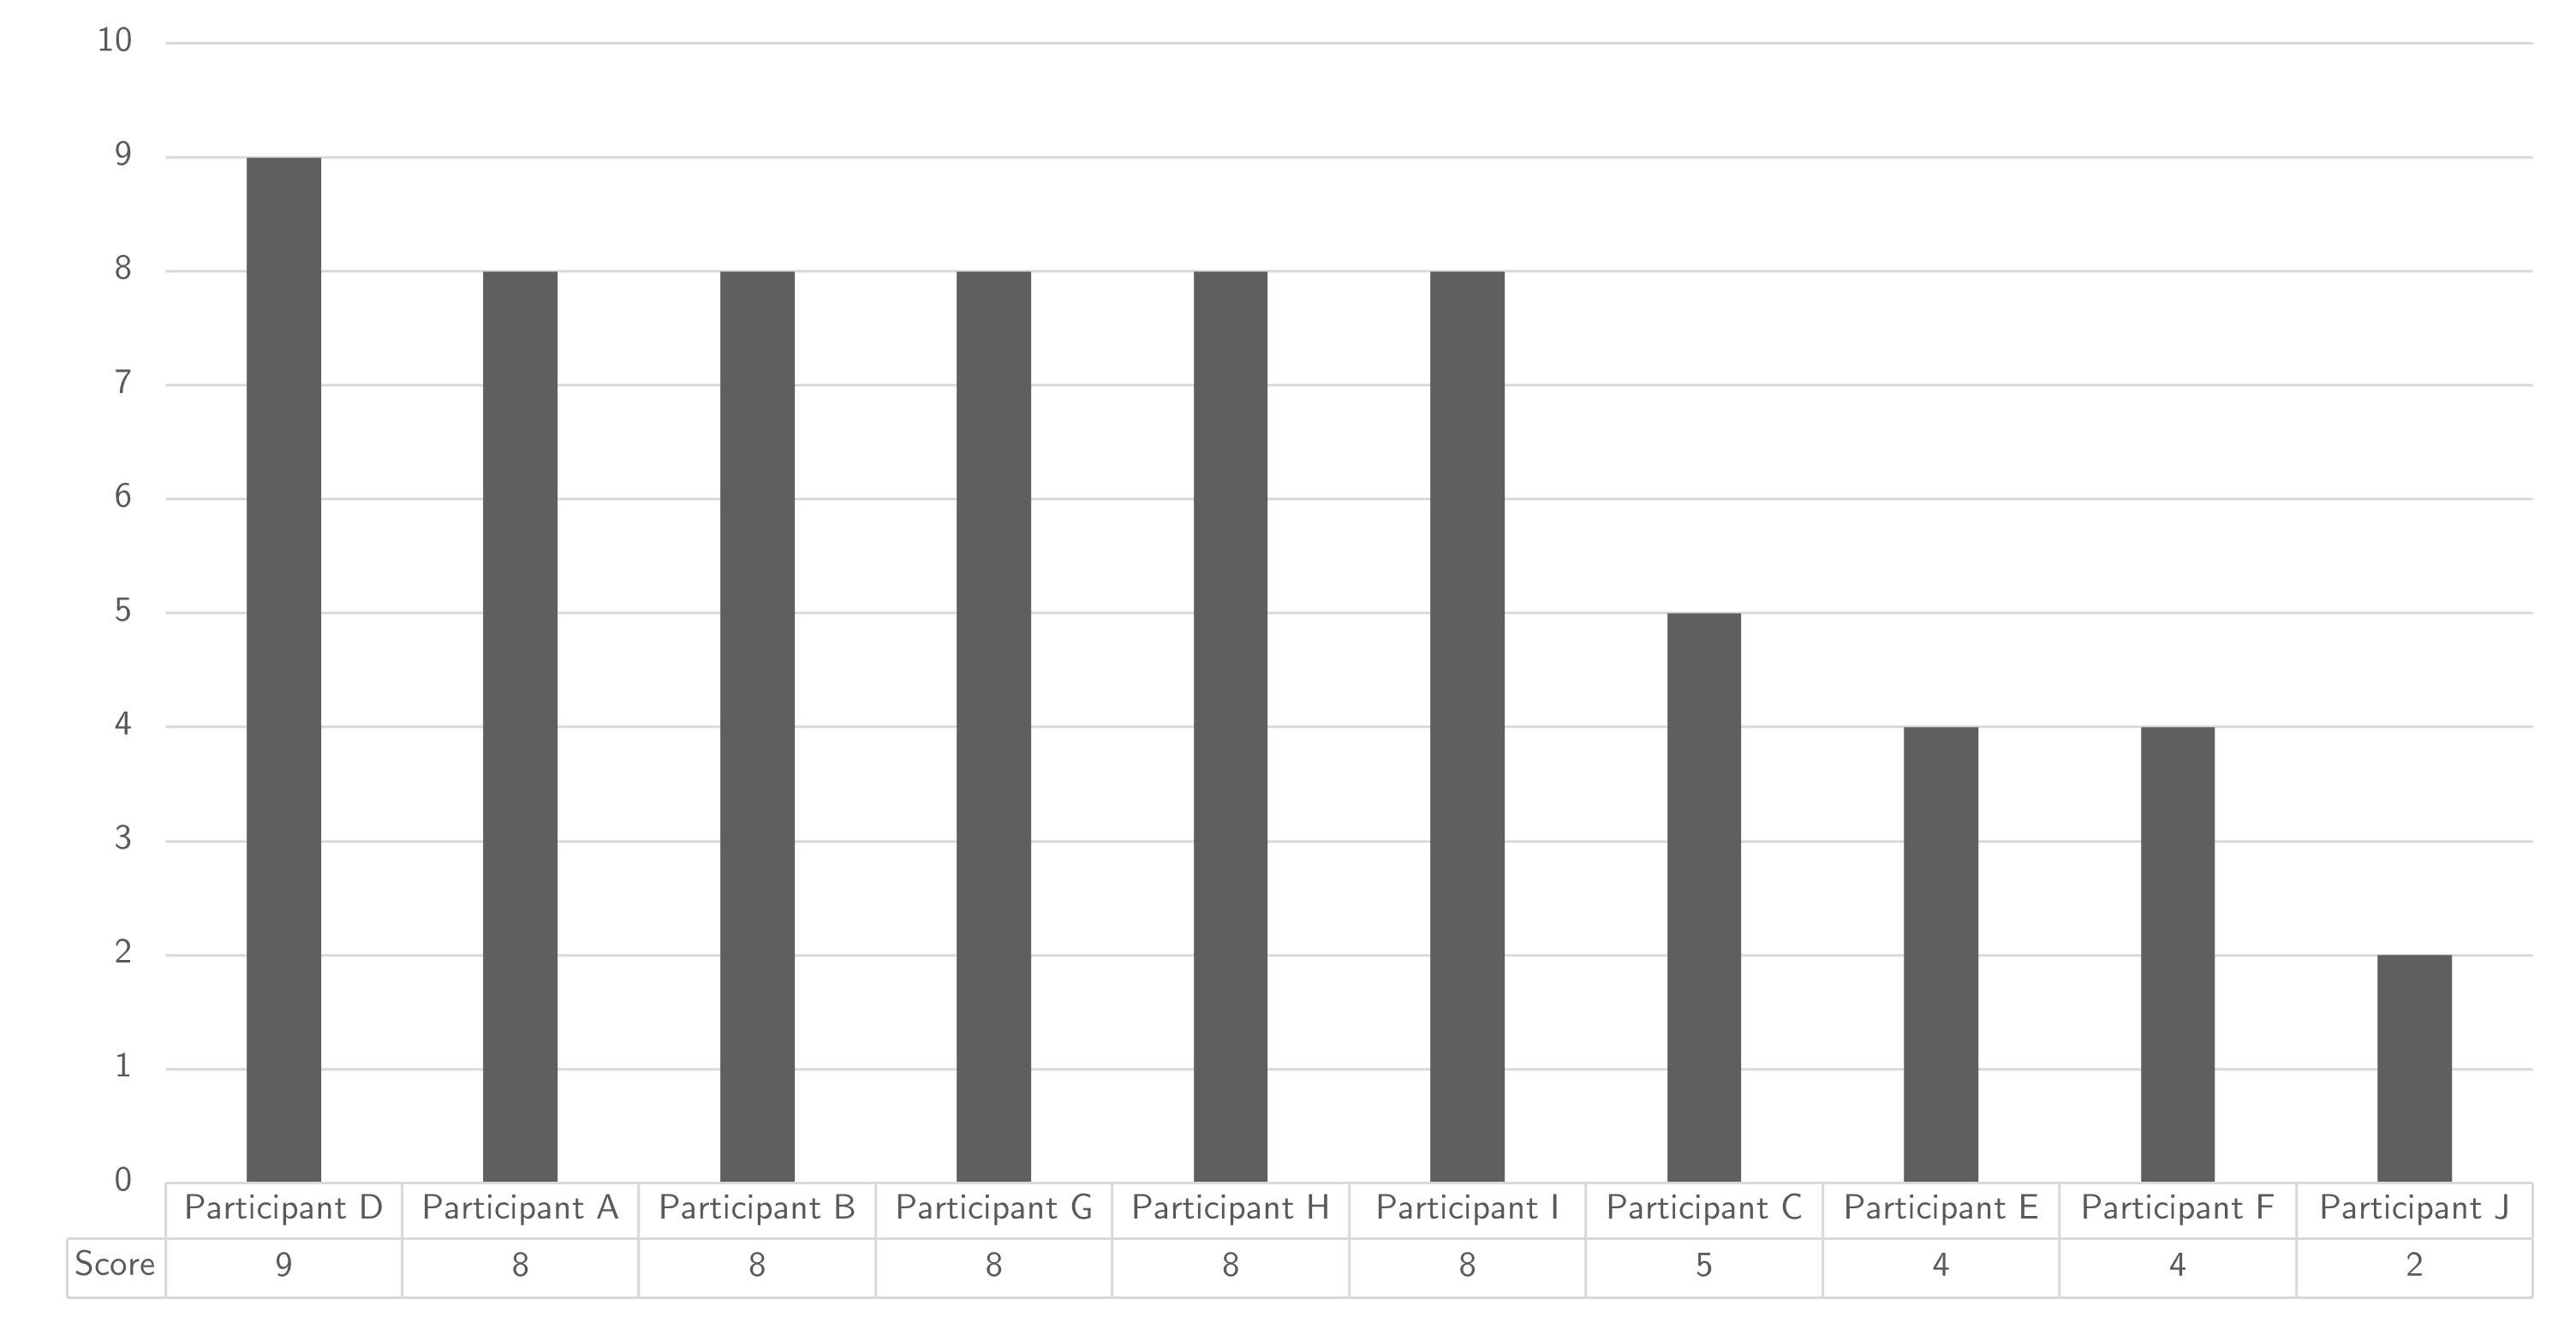
\includegraphics[width=0.9\linewidth]{images/scoreeaagileenterprise}
	\caption[Scoring of EA attribute Agile Enterprise]{Scoring of EA attribute Agile Enterprise}
	\label{fig:appscoringeaagileneterprise}
\end{figure}
\begin{table}[H]
	\centering
	\begin{tabular}{p{.55\textwidth}ccc}
		\toprule
		\textbf{Attribute} & \textbf{Rating} & \textbf{Variability} & \textbf{Abstains} \\
		\midrule
		Agile Enterprise & 6,4 & 50\% & 0 \\%
		\bottomrule
	\end{tabular}%
	\caption[Scoring of EA attribute Agile Enterprise]{Scoring of EA attribute Agile Enterprise}
	\label{tab:appscoringeaagileenterprise}%
\end{table}%
\newpage
\subsection{Real Time Trust}
\begin{figure}[H]
	\centering
	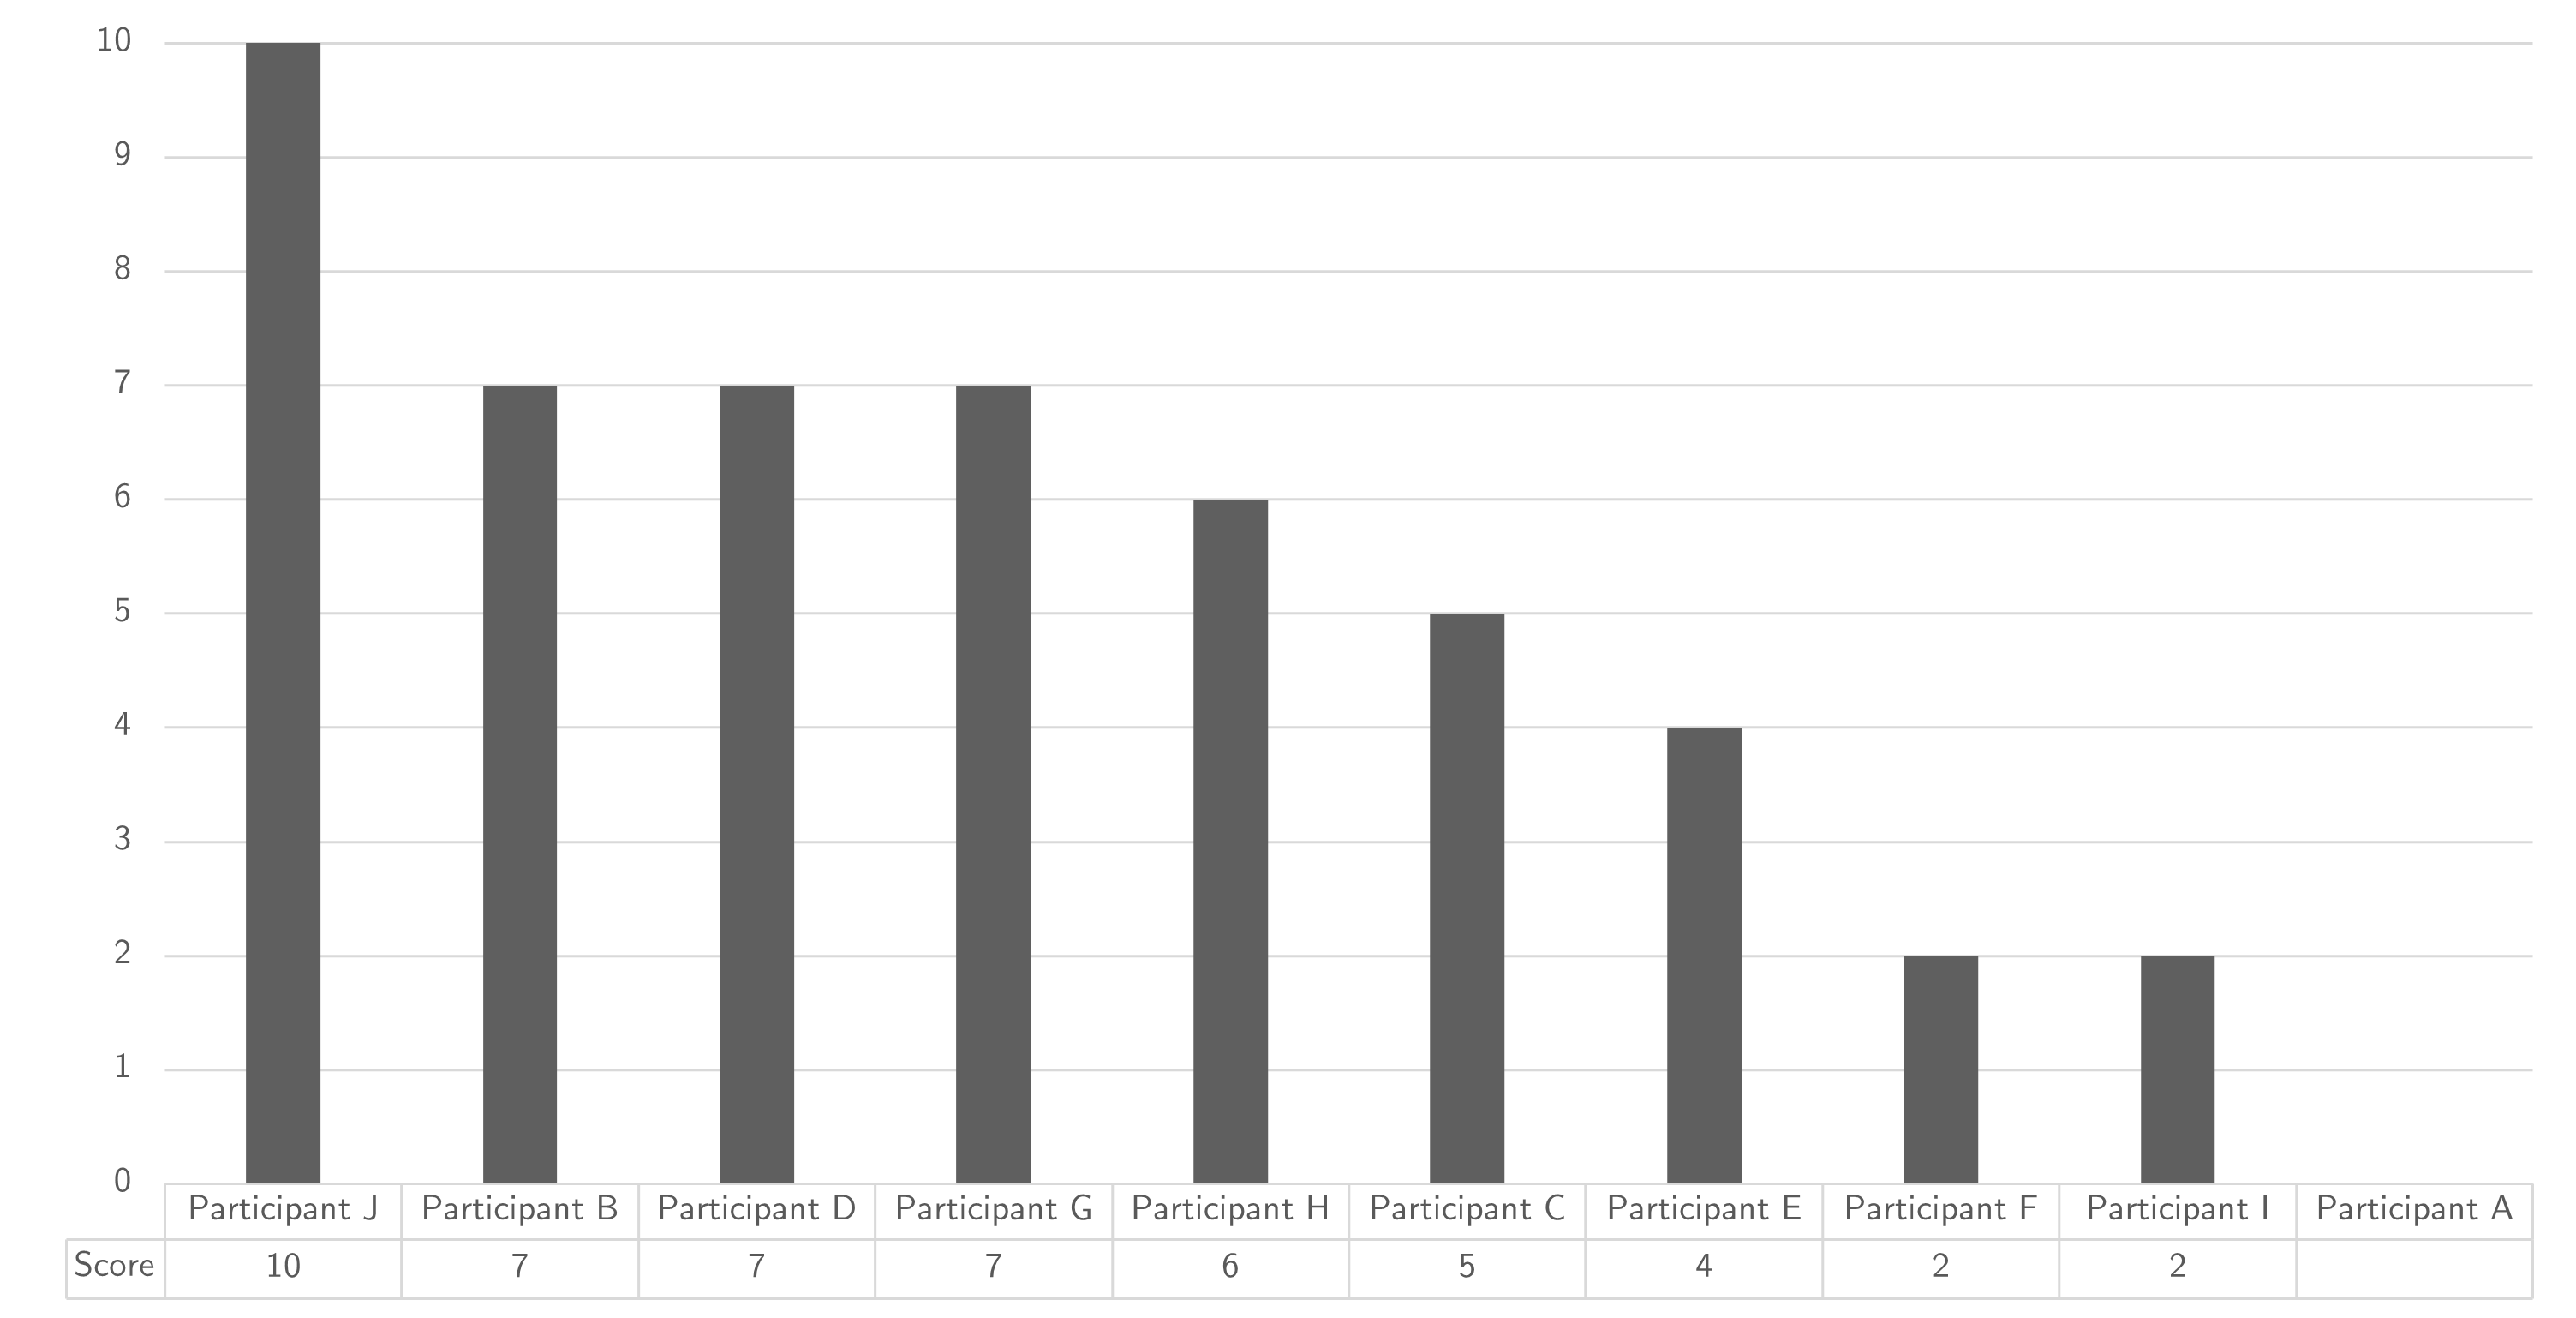
\includegraphics[width=0.9\linewidth]{images/scoreearealtimetrust}
	\caption[Scoring of EA attribute Real Time Trust]{Scoring of EA attribute Real Time Trust}
	\label{fig:appscoringearealtimetrust}
\end{figure}
\begin{table}[H]
	\centering
	\begin{tabular}{p{.55\textwidth}ccc}
		\toprule
		\textbf{Attribute} & \textbf{Rating} & \textbf{Variability} & \textbf{Abstains} \\
		\midrule
		Real Time Trust (Policy \& Attribute based) & 5,6 & 54\% & 1 \\%
		\bottomrule
	\end{tabular}%
	\caption[Scoring of EA attribute Real Time Trust]{Scoring of EA attribute Real Time Trust}
	\label{tab:appscoringearealtimetrust}%
\end{table}%
\newpage
\subsection{Foster Dialogue}
\begin{figure}[H]
	\centering
	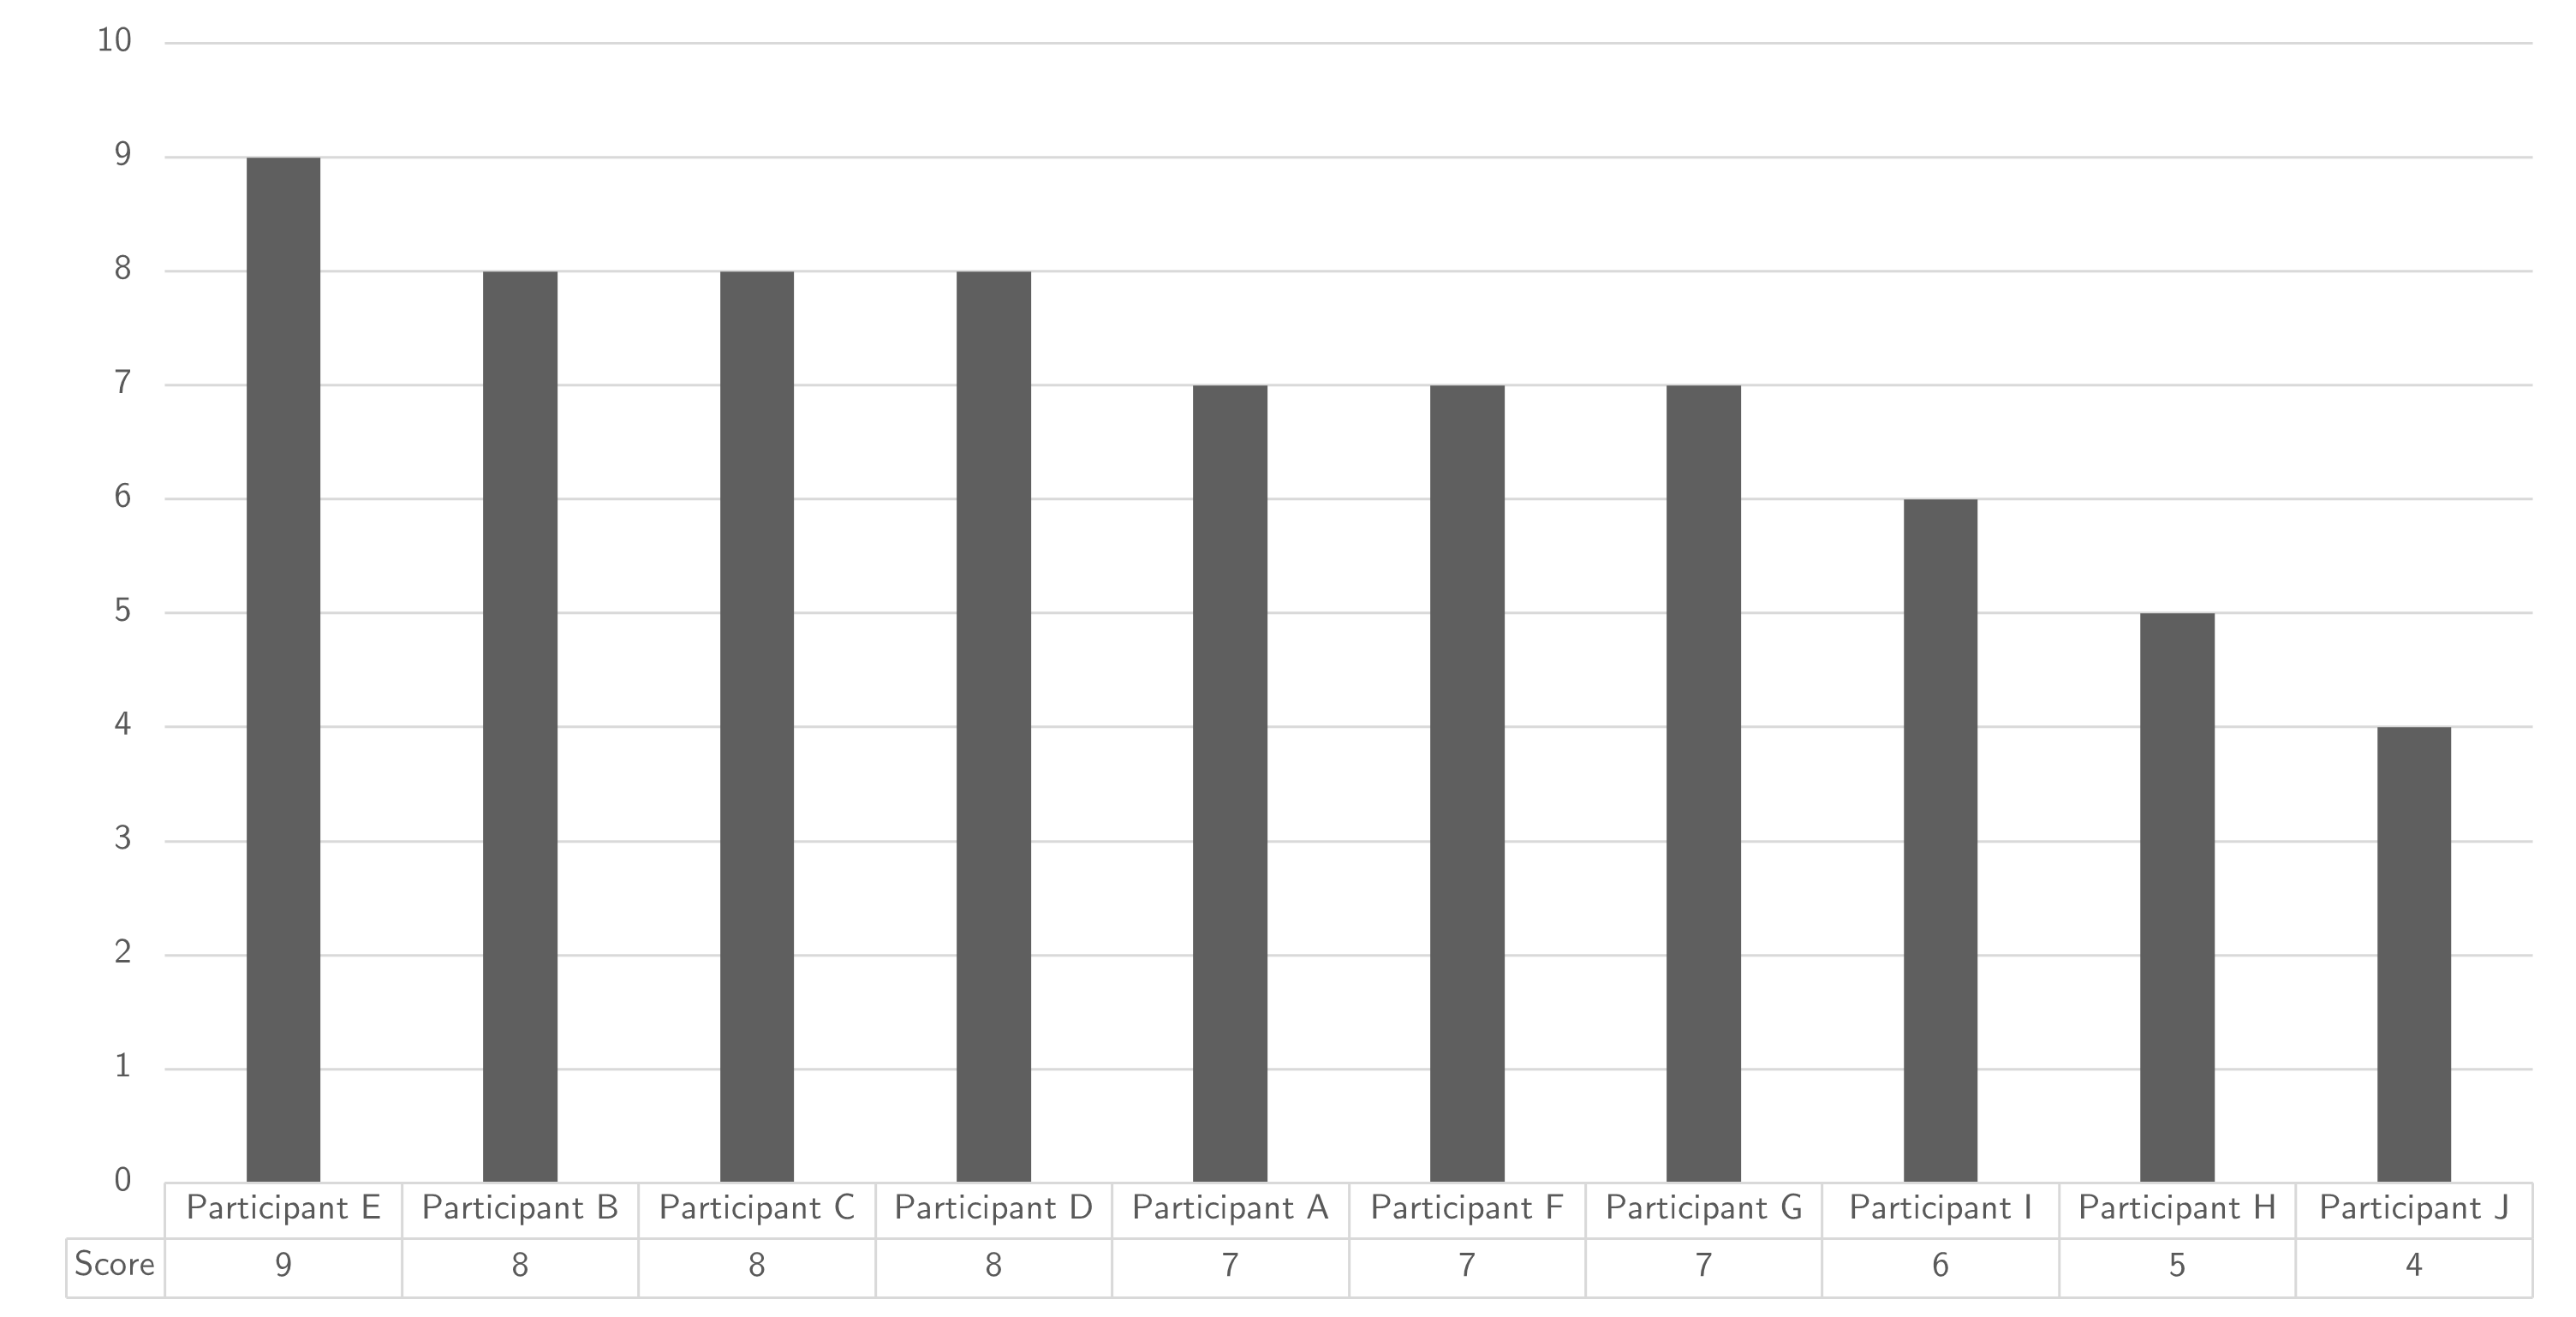
\includegraphics[width=0.9\linewidth]{images/scoreeafosterdialogue}
	\caption[Scoring of EA attribute Foster Dialogue]{Scoring of EA attribute Foster Dialogue}
	\label{fig:appscoringeafosterdialogue}
\end{figure}
\begin{table}[H]
	\centering
	\begin{tabular}{p{.55\textwidth}ccc}
		\toprule
		\textbf{Attribute} & \textbf{Rating} & \textbf{Variability} & \textbf{Abstains} \\
		\midrule
		Foster Dialogue & 6,9 & 32\% & 0 \\%
		\bottomrule
	\end{tabular}%
	\caption[Scoring of EA attribute Foster Dialogue]{Scoring of EA attribute Foster Dialogue}
	\label{tab:appscoringeafosterdialogue}%
\end{table}%
\newpage
\subsection{Architecture validation}
\begin{figure}[H]
	\centering
	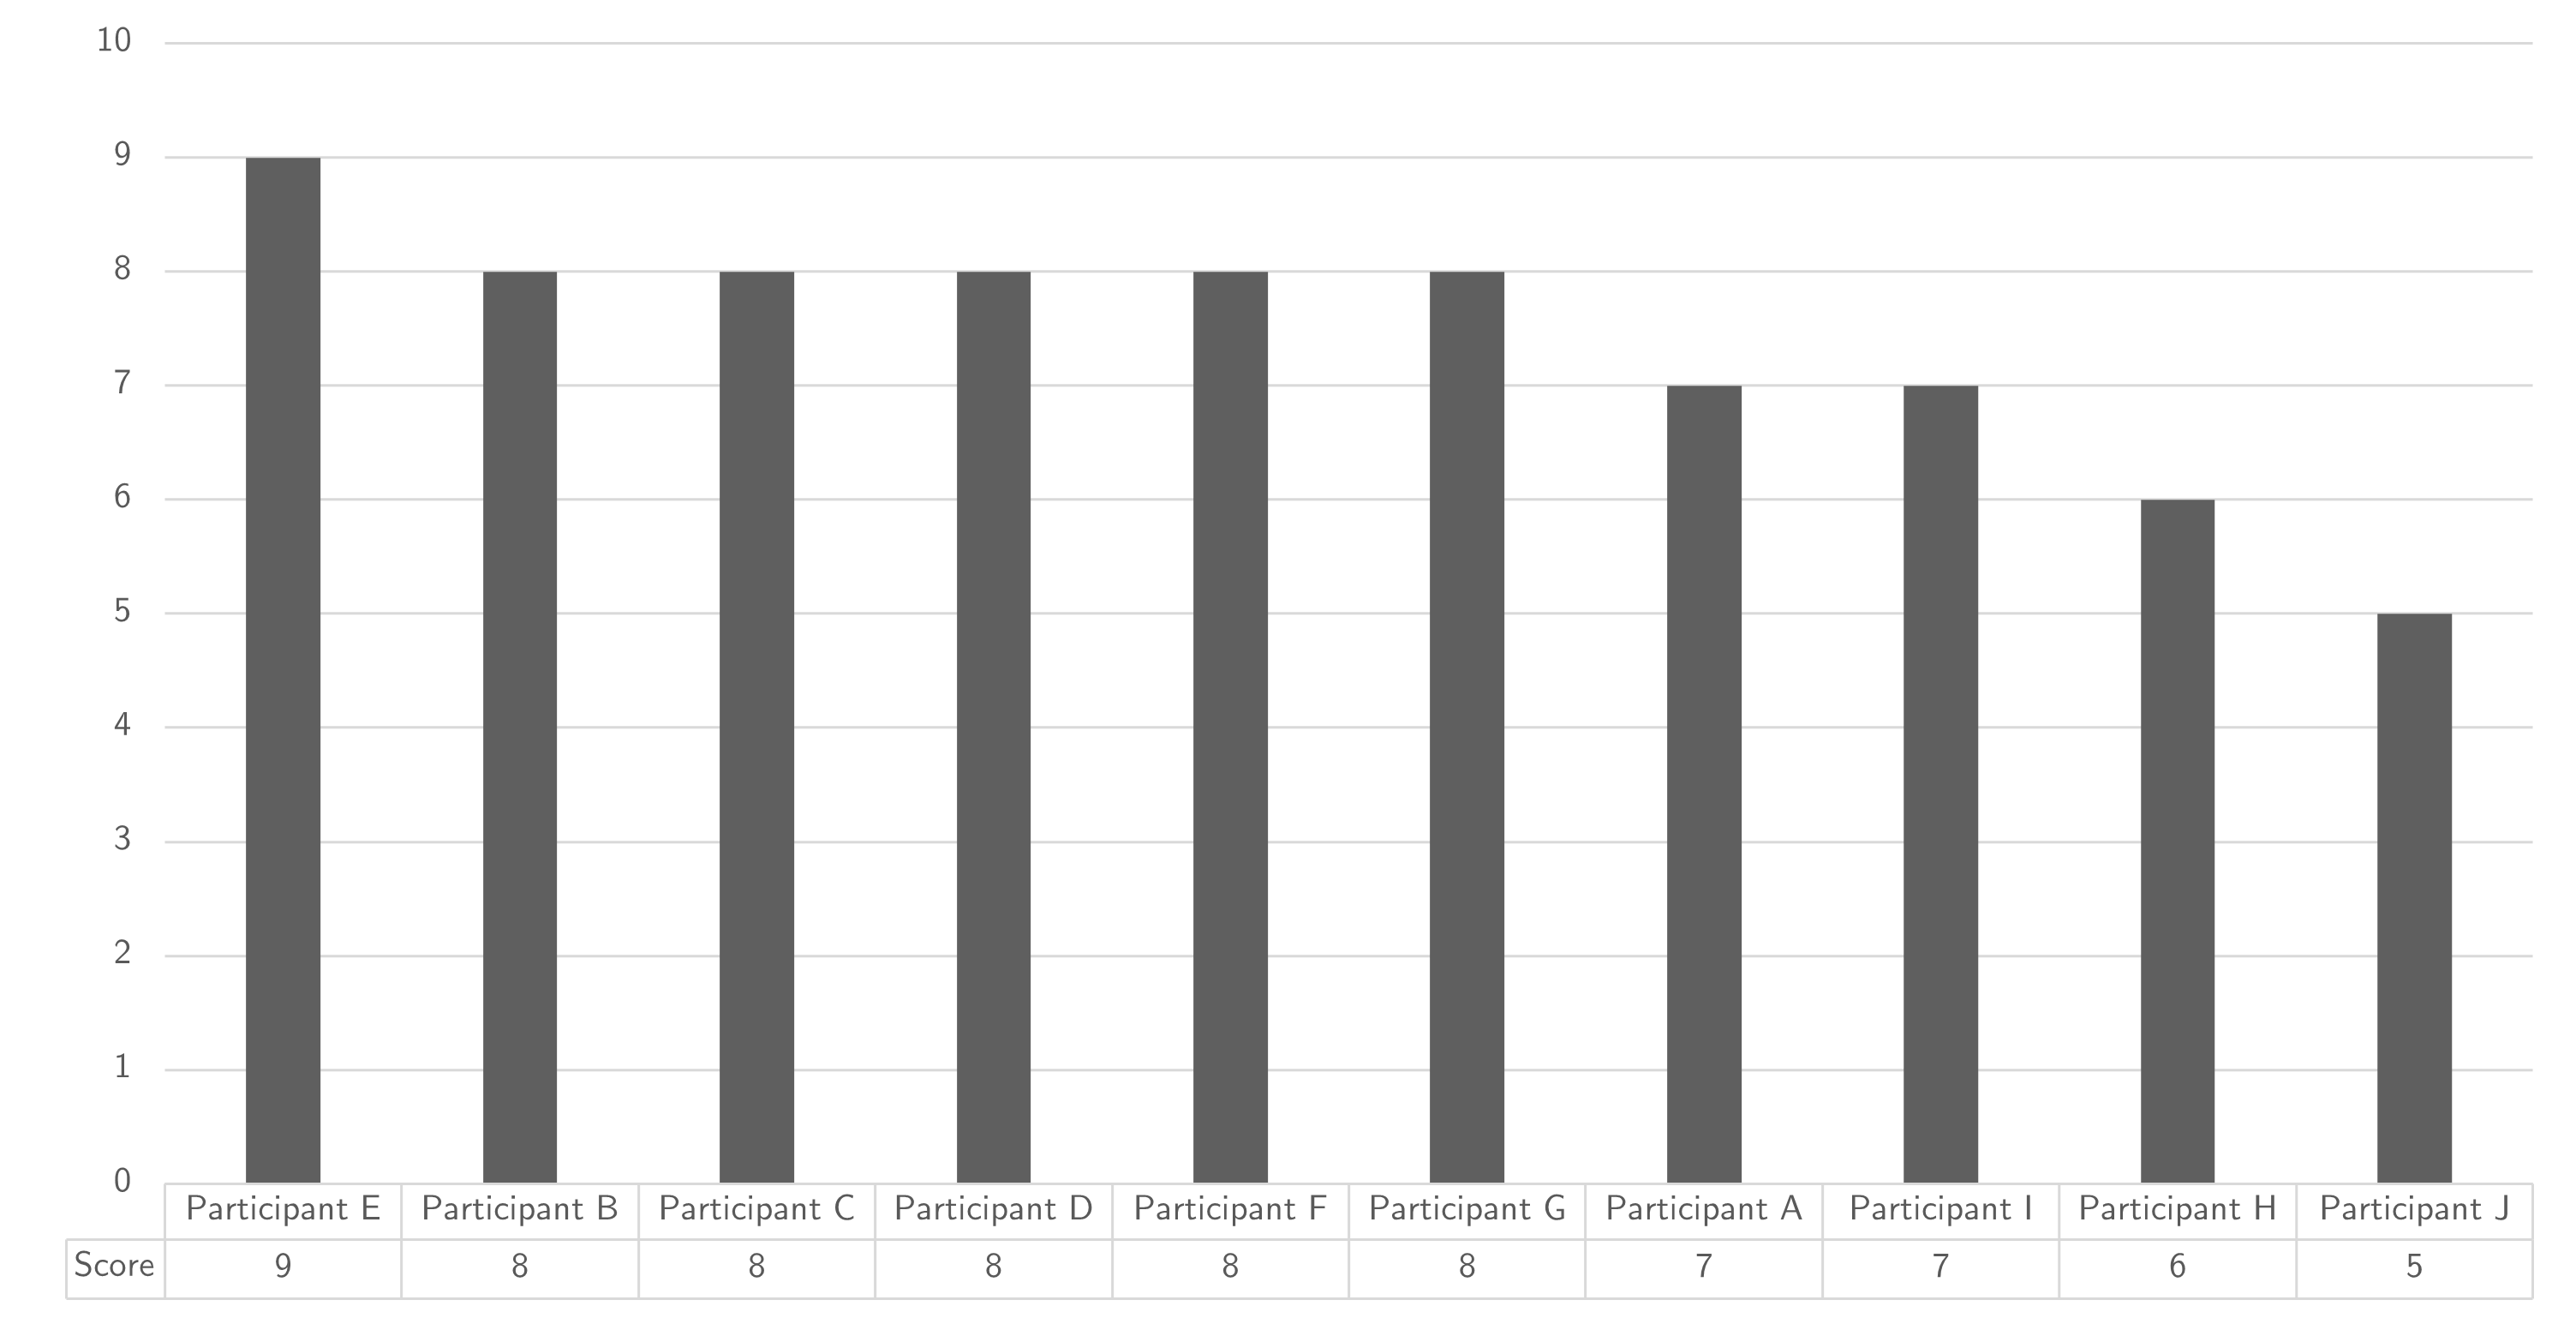
\includegraphics[width=0.9\linewidth]{images/scoreeavalidation}
	\caption[Scoring of EA attribute Architecture validation]{Scoring of EA attribute Architecture validation}
	\label{fig:appscoringeavalidation}
\end{figure}
\begin{table}[H]
	\centering
	\begin{tabular}{p{.55\textwidth}ccc}
		\toprule
		\textbf{Attribute} & \textbf{Rating} & \textbf{Variability} & \textbf{Abstains} \\
		\midrule
		Validation & 7,4 & 24\% & 0 \\%
		\bottomrule
	\end{tabular}%
	\caption[Scoring of EA attribute Architecture validation]{Scoring of EA attribute Architecture validation}
	\label{tab:appscoringeavalidation}%
\end{table}%
\newpage
\subsection{Always fitting Enterprise Architecture}
\begin{figure}[H]
	\centering
	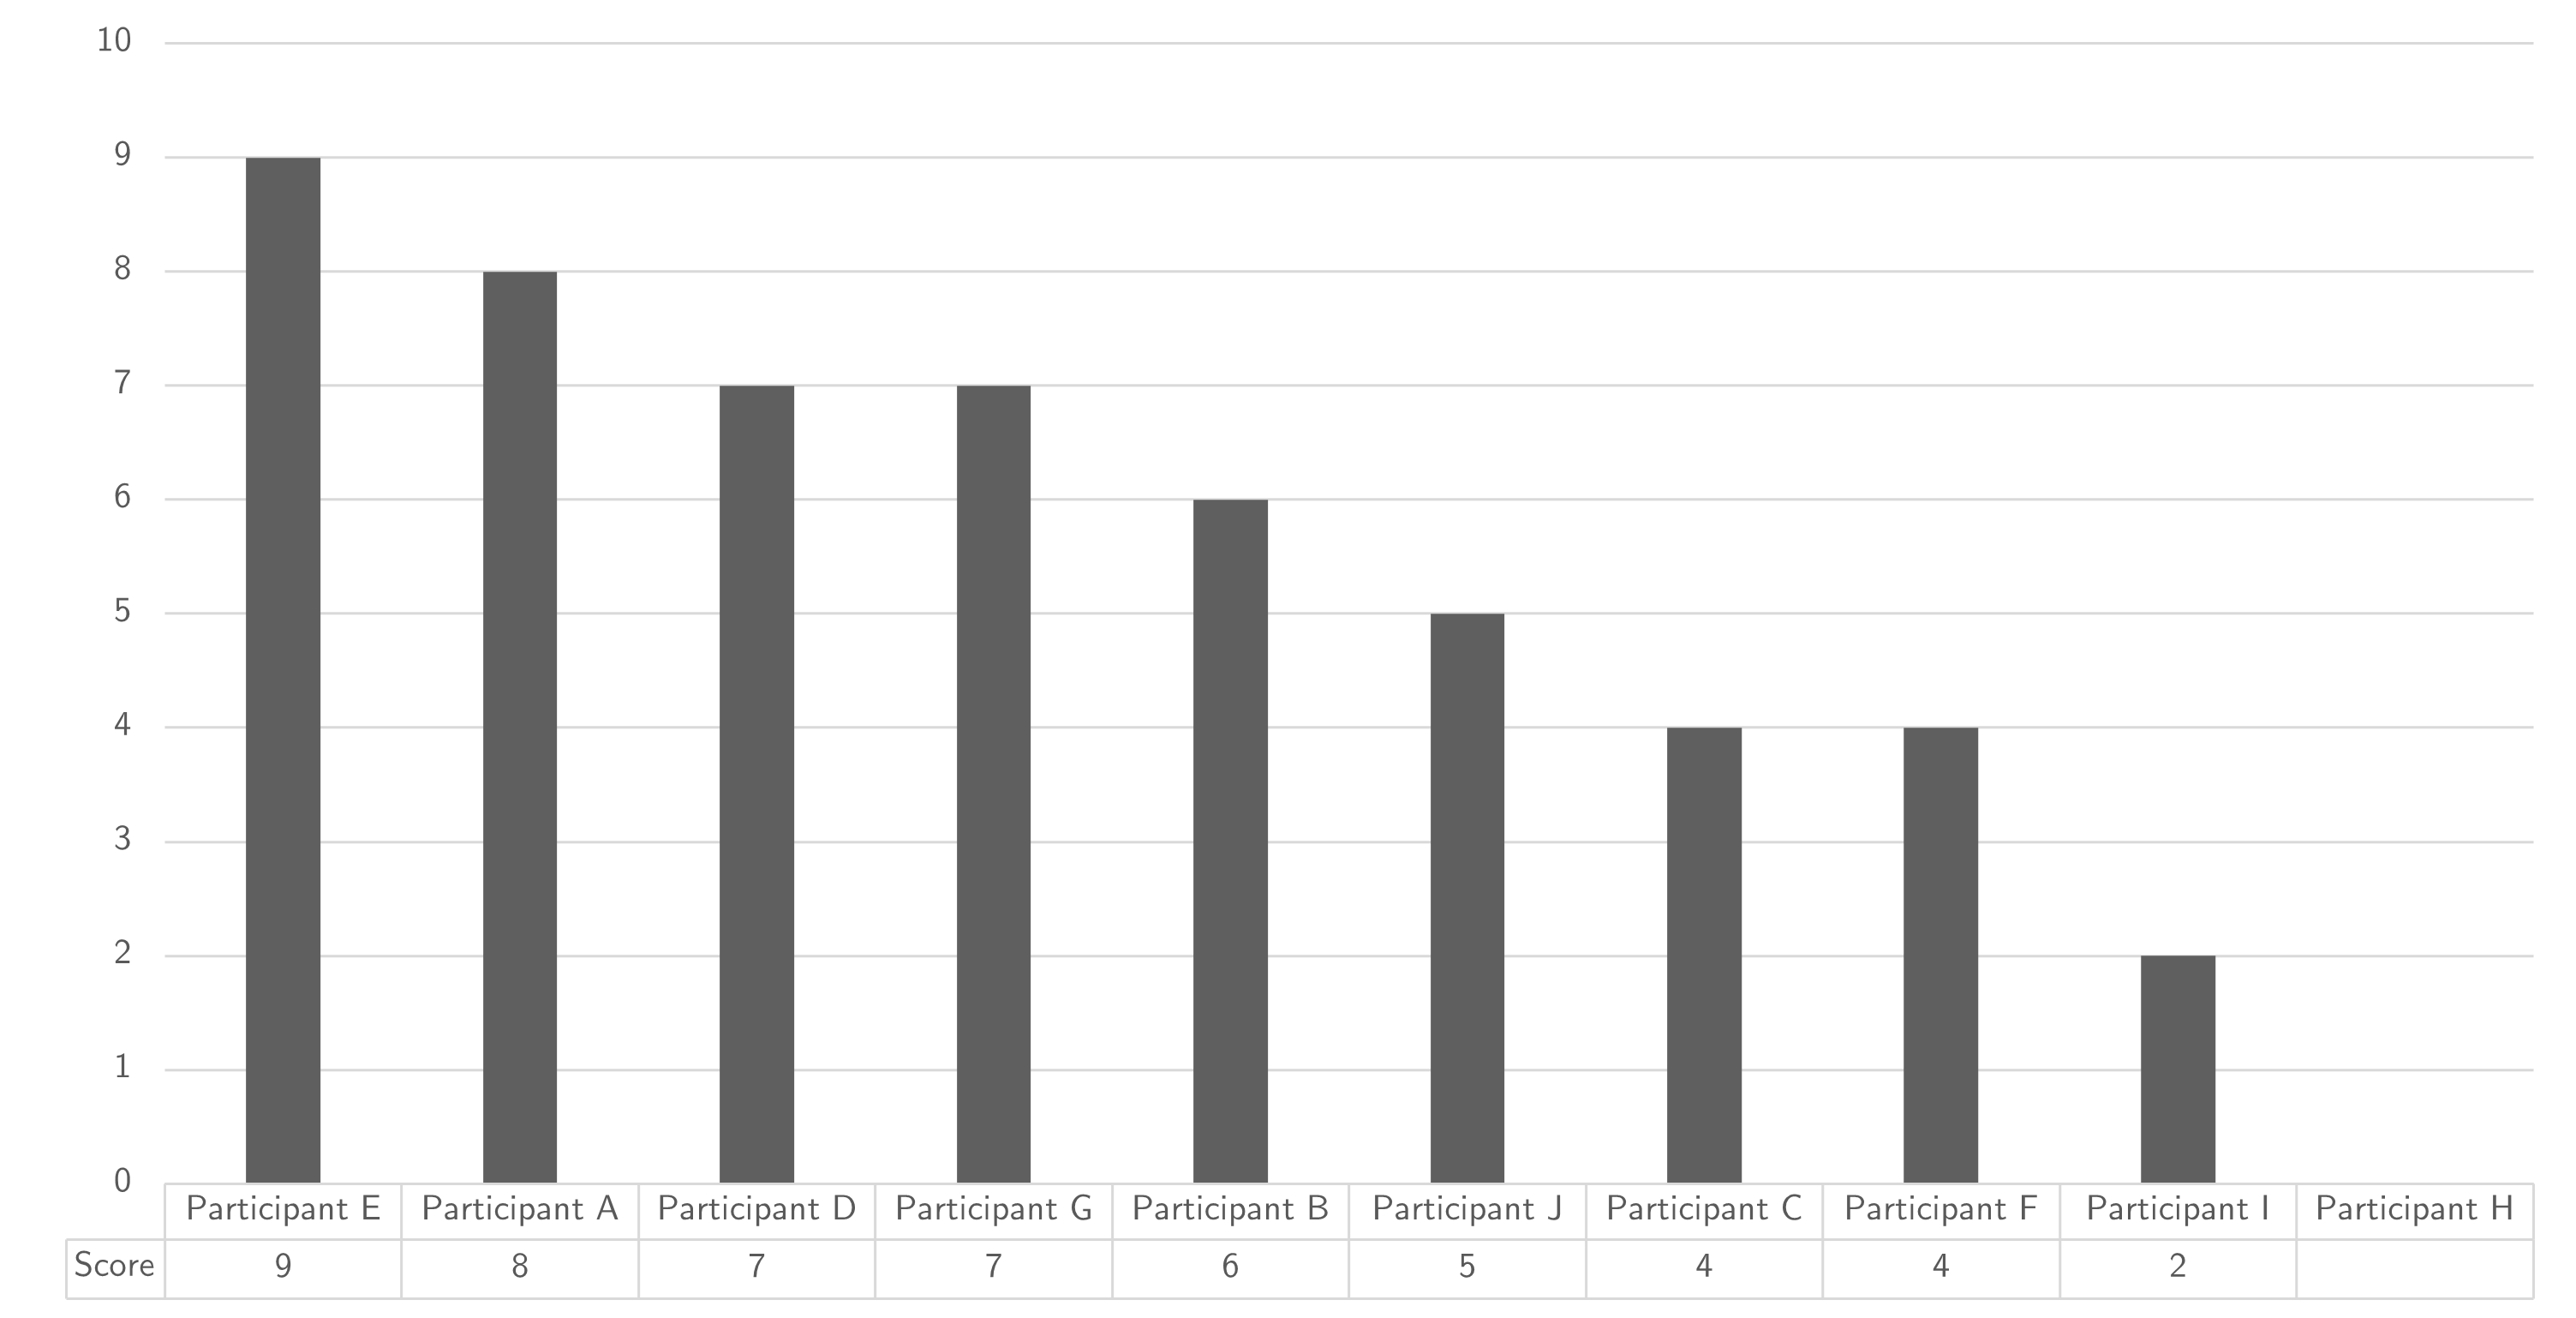
\includegraphics[width=0.9\linewidth]{images/scoreeaalwaysfitea}
	\caption[Scoring of EA attribute Always fitting EA]{Scoring of EA attribute Always fitting EA}
	\label{fig:appscoringeaalwaysfitea}
\end{figure}
\begin{table}[H]
	\centering
	\begin{tabular}{p{.55\textwidth}ccc}
		\toprule
		\textbf{Attribute} & \textbf{Rating} & \textbf{Variability} & \textbf{Abstains} \\
		\midrule
		Always fitting EA & 5,8 & 46\% & 1 \\%
		\bottomrule
	\end{tabular}%
	\caption[Scoring of EA attribute Always fitting EA]{Scoring of EA attribute Always fitting EA}
	\label{tab:appscoringeaalwaysfitea}%
\end{table}%

\section{Relevance of the research}
\label{sec:relevanceofresearchandexpectations}

\subsection{To what extent do you find the research relevant?}
\label{sub:relevantgeneric}

\begin{figure}[H]
	\centering
	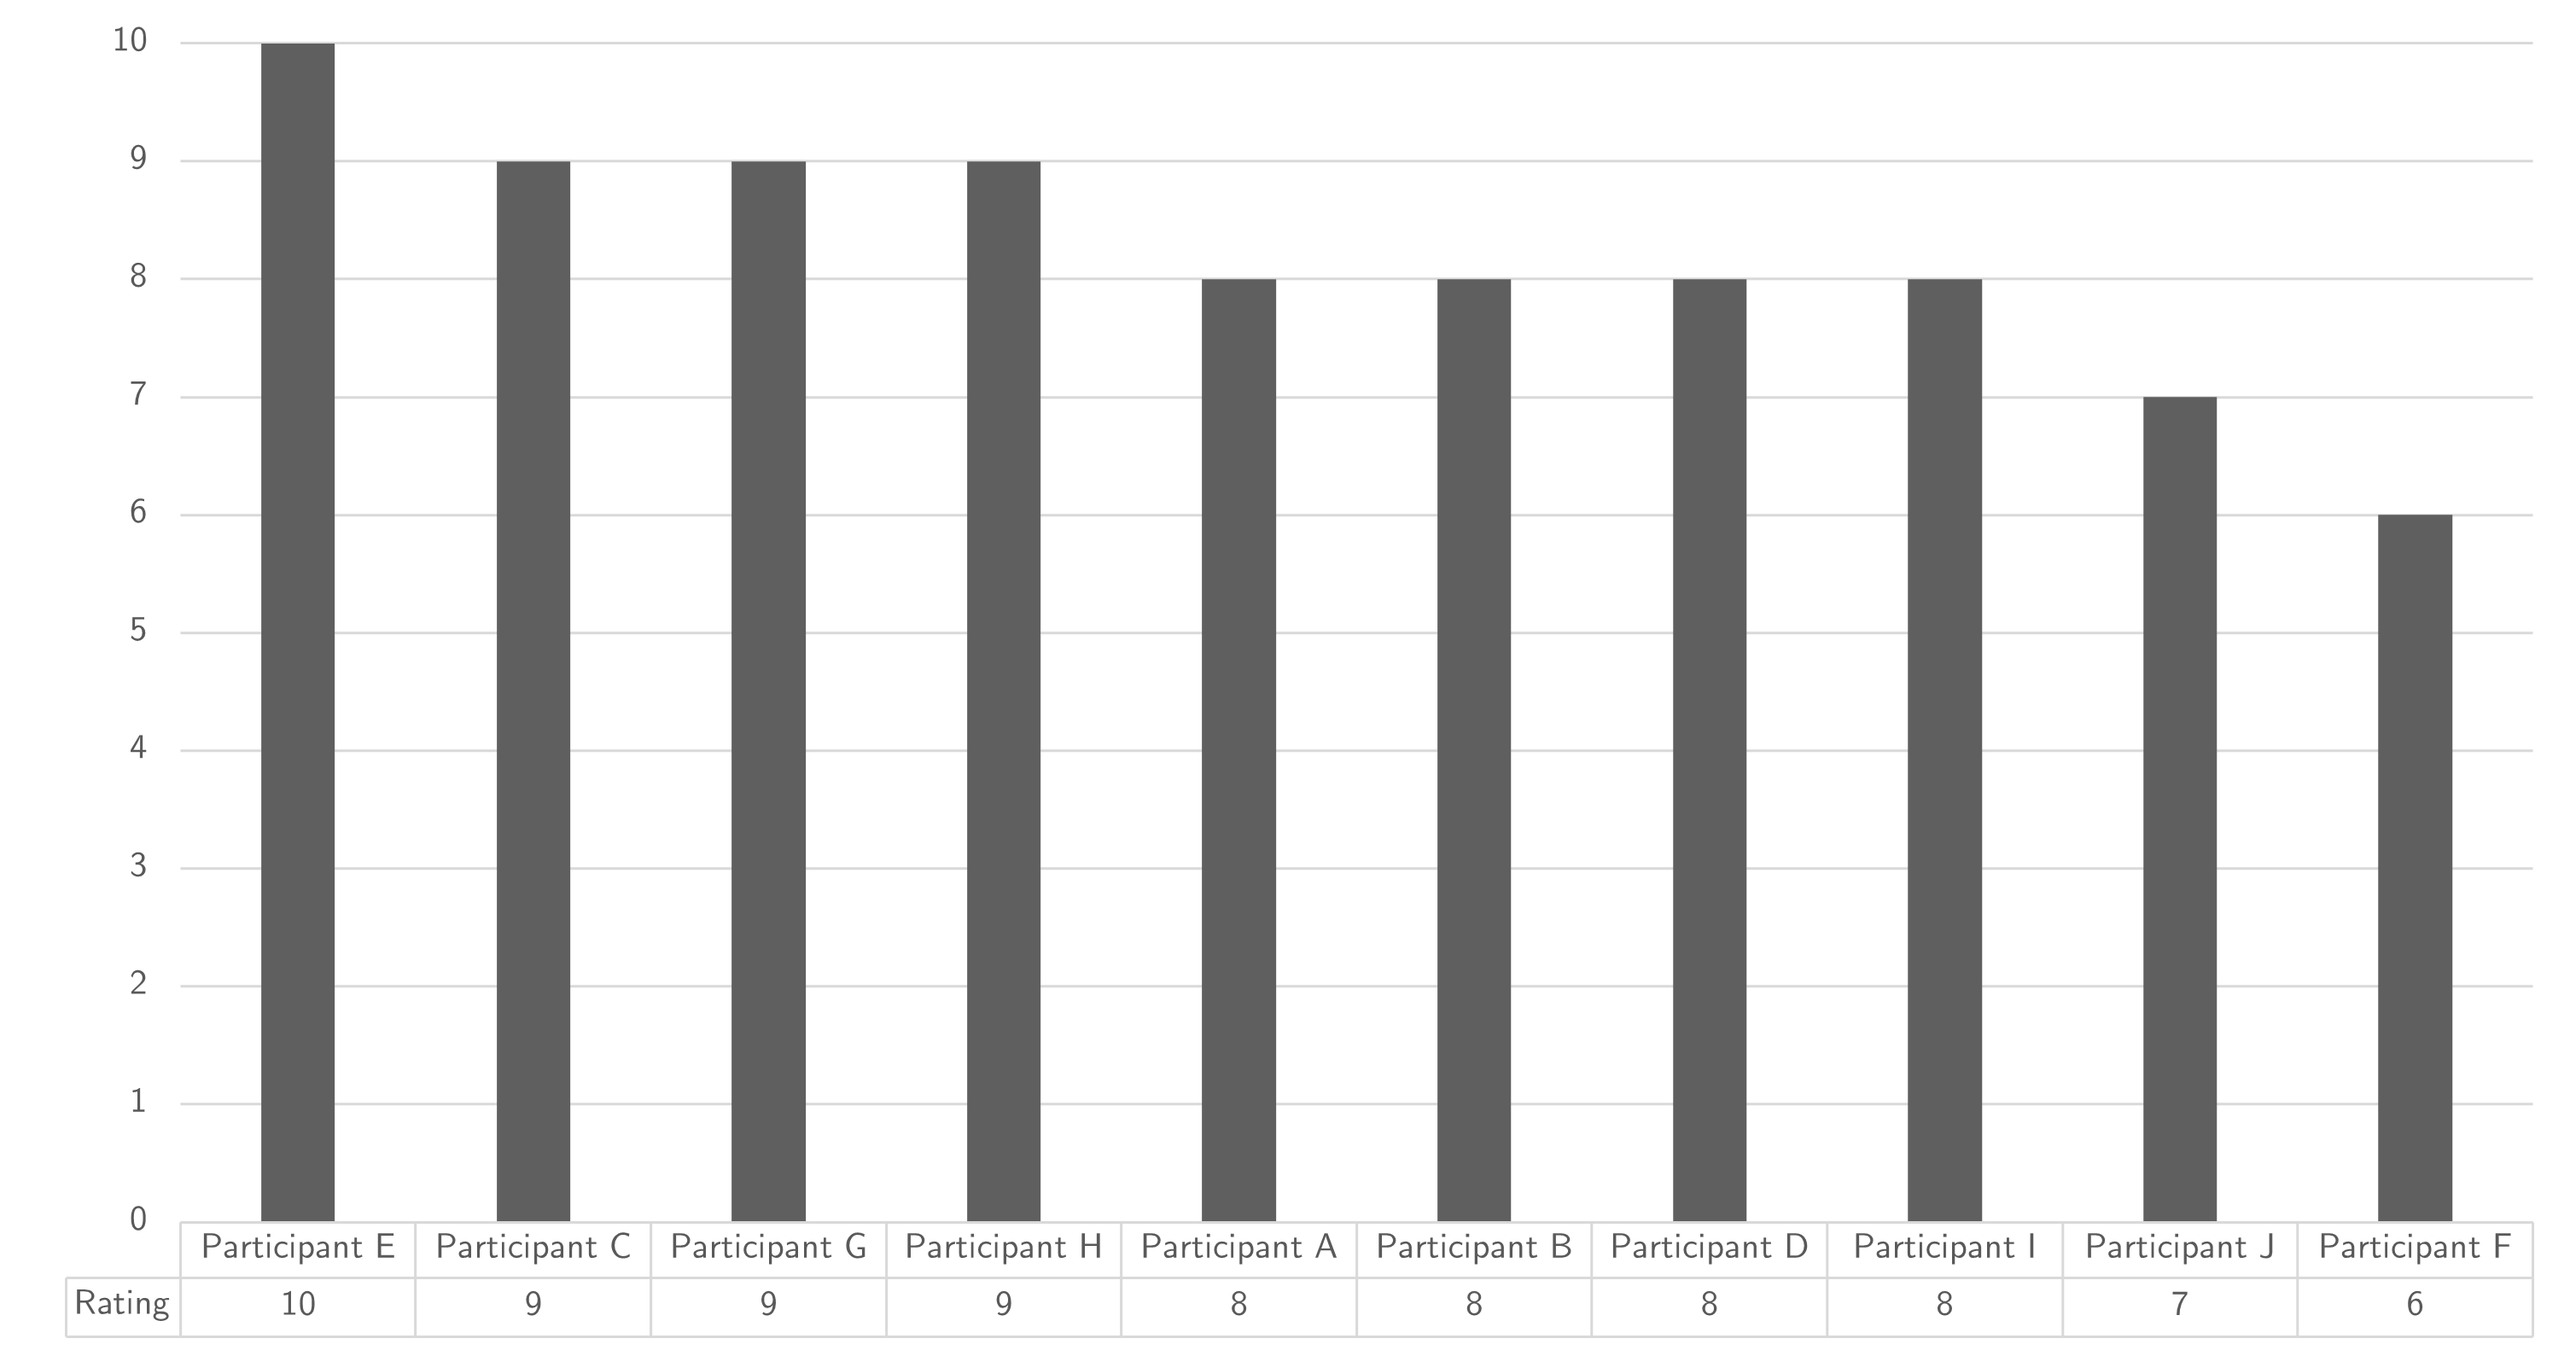
\includegraphics[width=0.9\linewidth]{images/validationresult_generalresearchrelevance}
	\caption[To what extent do you find the the research relevant?]{To what extent do you find the the research relevant?}
	\label{fig:validationrelevancegeneric}
\end{figure}
\begin{table}[H]
	\centering
	\begin{tabular}{p{.55\textwidth}ccc}
		\toprule
		\textbf{Question} & \textbf{Rating} & \textbf{Variability} & \textbf{Abstains} \\
		\midrule
		To what extent do you find the the research relevant? & 8,2 & 23\% & 0 \\%
		\bottomrule
	\end{tabular}%
	\caption[To what extent do you find the the research relevant?]{To what extent do you find the the research relevant?}
	\label{tab:validationrelevancegeneric}%
\end{table}%

\subsection{To what extent did this session fulfil your expectations?}
\label{sub:fulfilexpectations}

\begin{figure}[H]
	\centering
	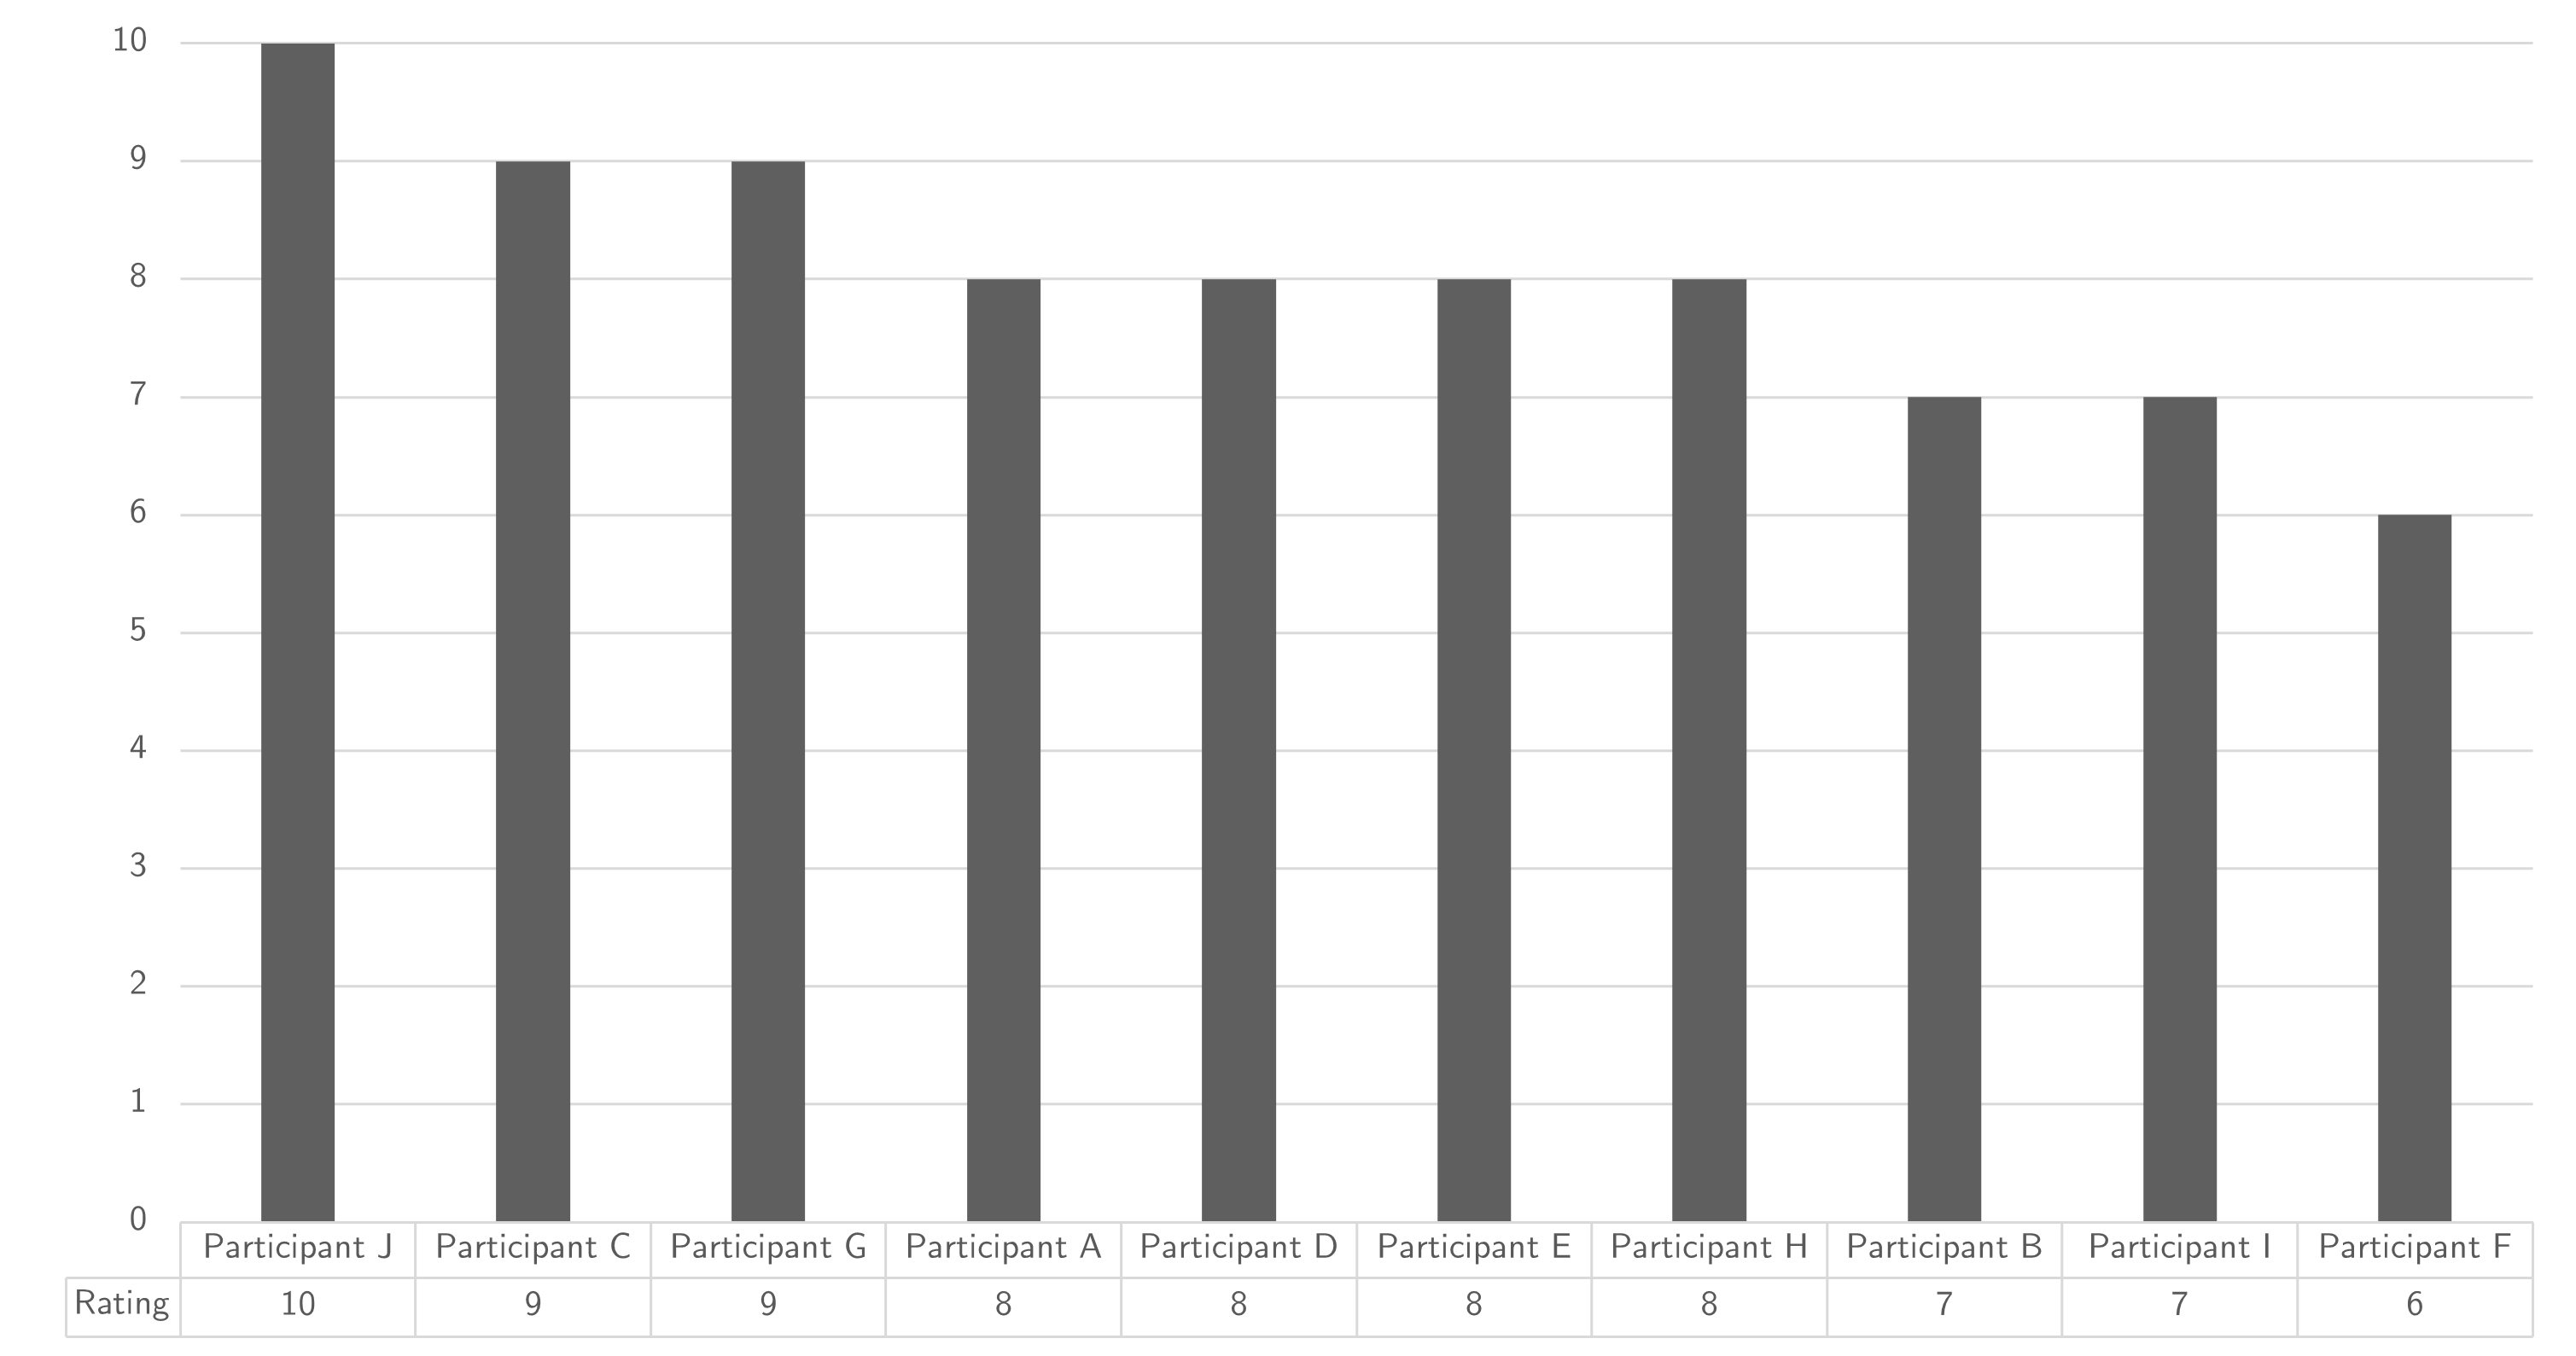
\includegraphics[width=0.9\linewidth]{images/validationresult_fulfilexpectations}
	\caption[To what extent did this session fulfil your expectations?]{To what extent did this session fulfil your expectations?}
	\label{fig:fulfilexpectations}
\end{figure}
\begin{table}[H]
	\centering
	\begin{tabular}{p{.55\textwidth}ccc}
		\toprule
		\textbf{Question} & \textbf{Rating} & \textbf{Variability} & \textbf{Abstains} \\
		\midrule
		To what extent did this session fulfil your expectations? & 8,2 & 23\% & 0 \\%
		\bottomrule
	\end{tabular}%
	\caption[To what extent did this session fulfil your expectations?]{To what extent did this session fulfil your expectations?}
	\label{tab:fulfilexpectations}%
\end{table}%

\subsection{To what extent do you think that the research can be used by yourself?}
\label{sub:validationrelevantyourself}

\begin{figure}[H]
	\centering
	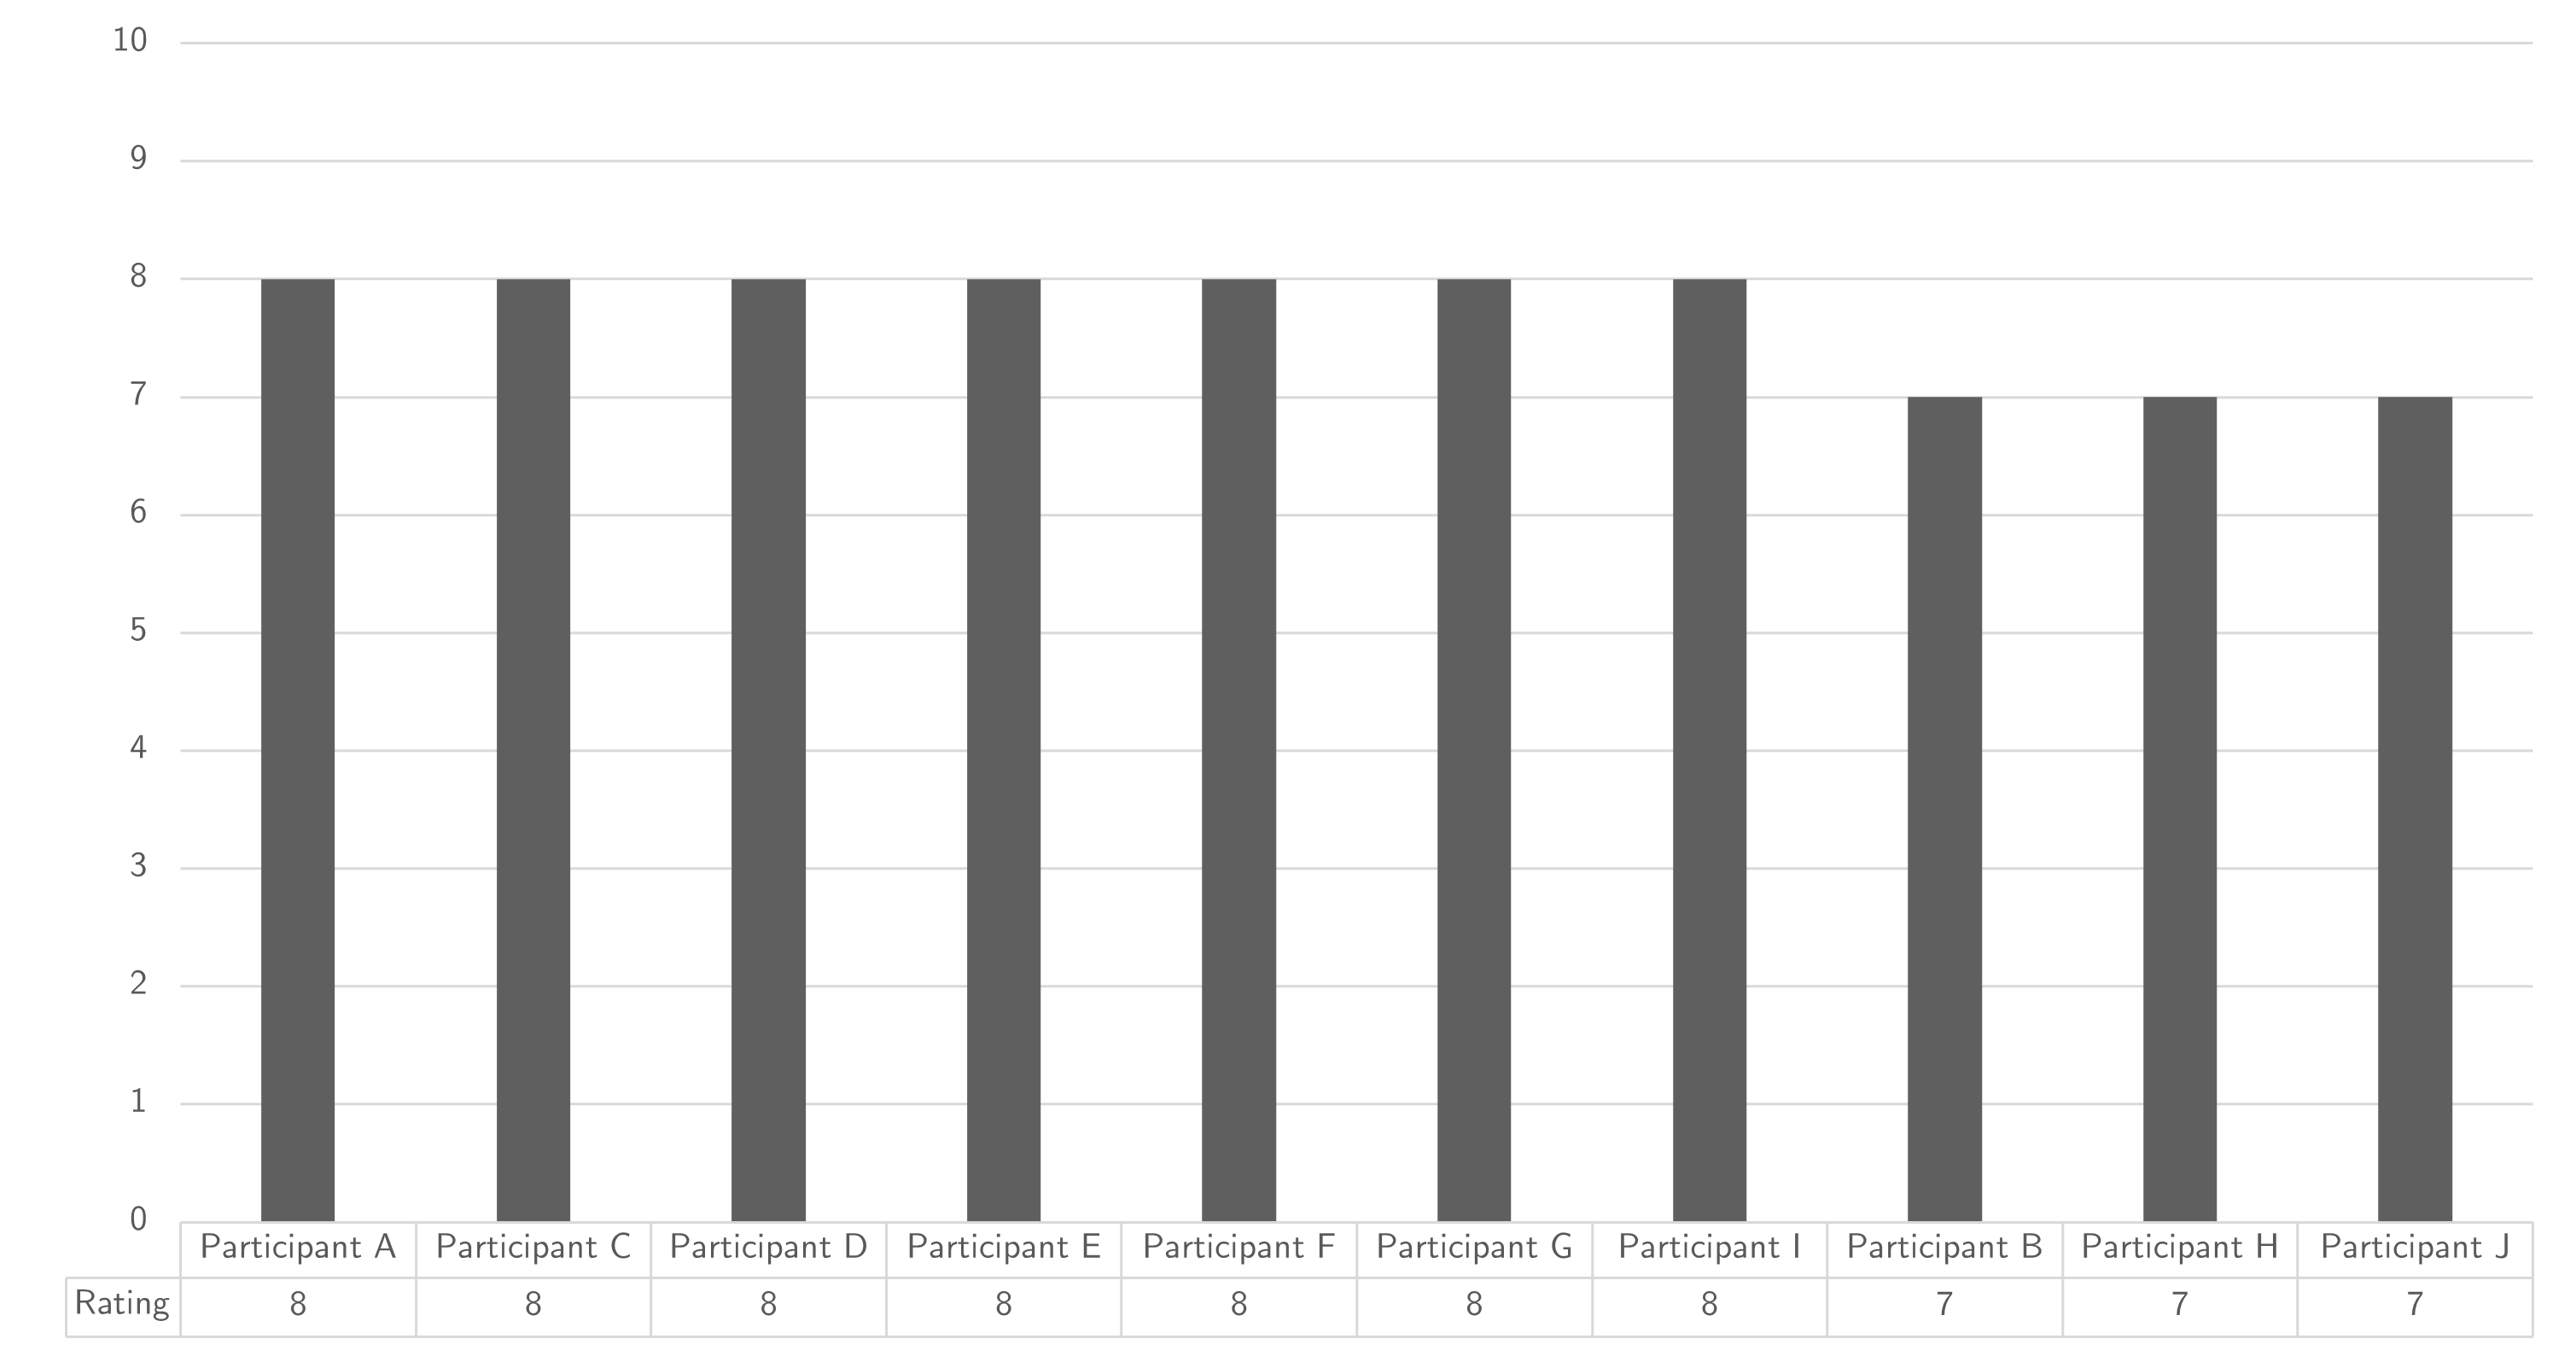
\includegraphics[width=0.9\linewidth]{images/validationresult_researchrelevanceexpert}
	\caption[To what extent do you think that the research can be used by yourself?]{To what extent do you think that the research can be used by yourself?}
	\label{fig:validationrelevantyourself}
\end{figure}
\begin{table}[H]
	\centering
	\begin{tabular}{p{.55\textwidth}ccc}
		\toprule
		\textbf{Question} & \textbf{Rating} & \textbf{Variability} & \textbf{Abstains} \\
		\midrule
		To what extent do you think that the research can be used by yourself? & 8,2 & 23\% & 0 \\%
		\bottomrule
	\end{tabular}%
	\caption[To what extent do you think that the research can be used by yourself?]{To what extent do you think that the research can be used by yourself?}
	\label{tab:validationrelevantyourself}%
\end{table}%

\subsection{To what extent do you think that the research can be used in the public sector?}
\label{sub:validationrelevantps}

\begin{figure}[H]
	\centering
	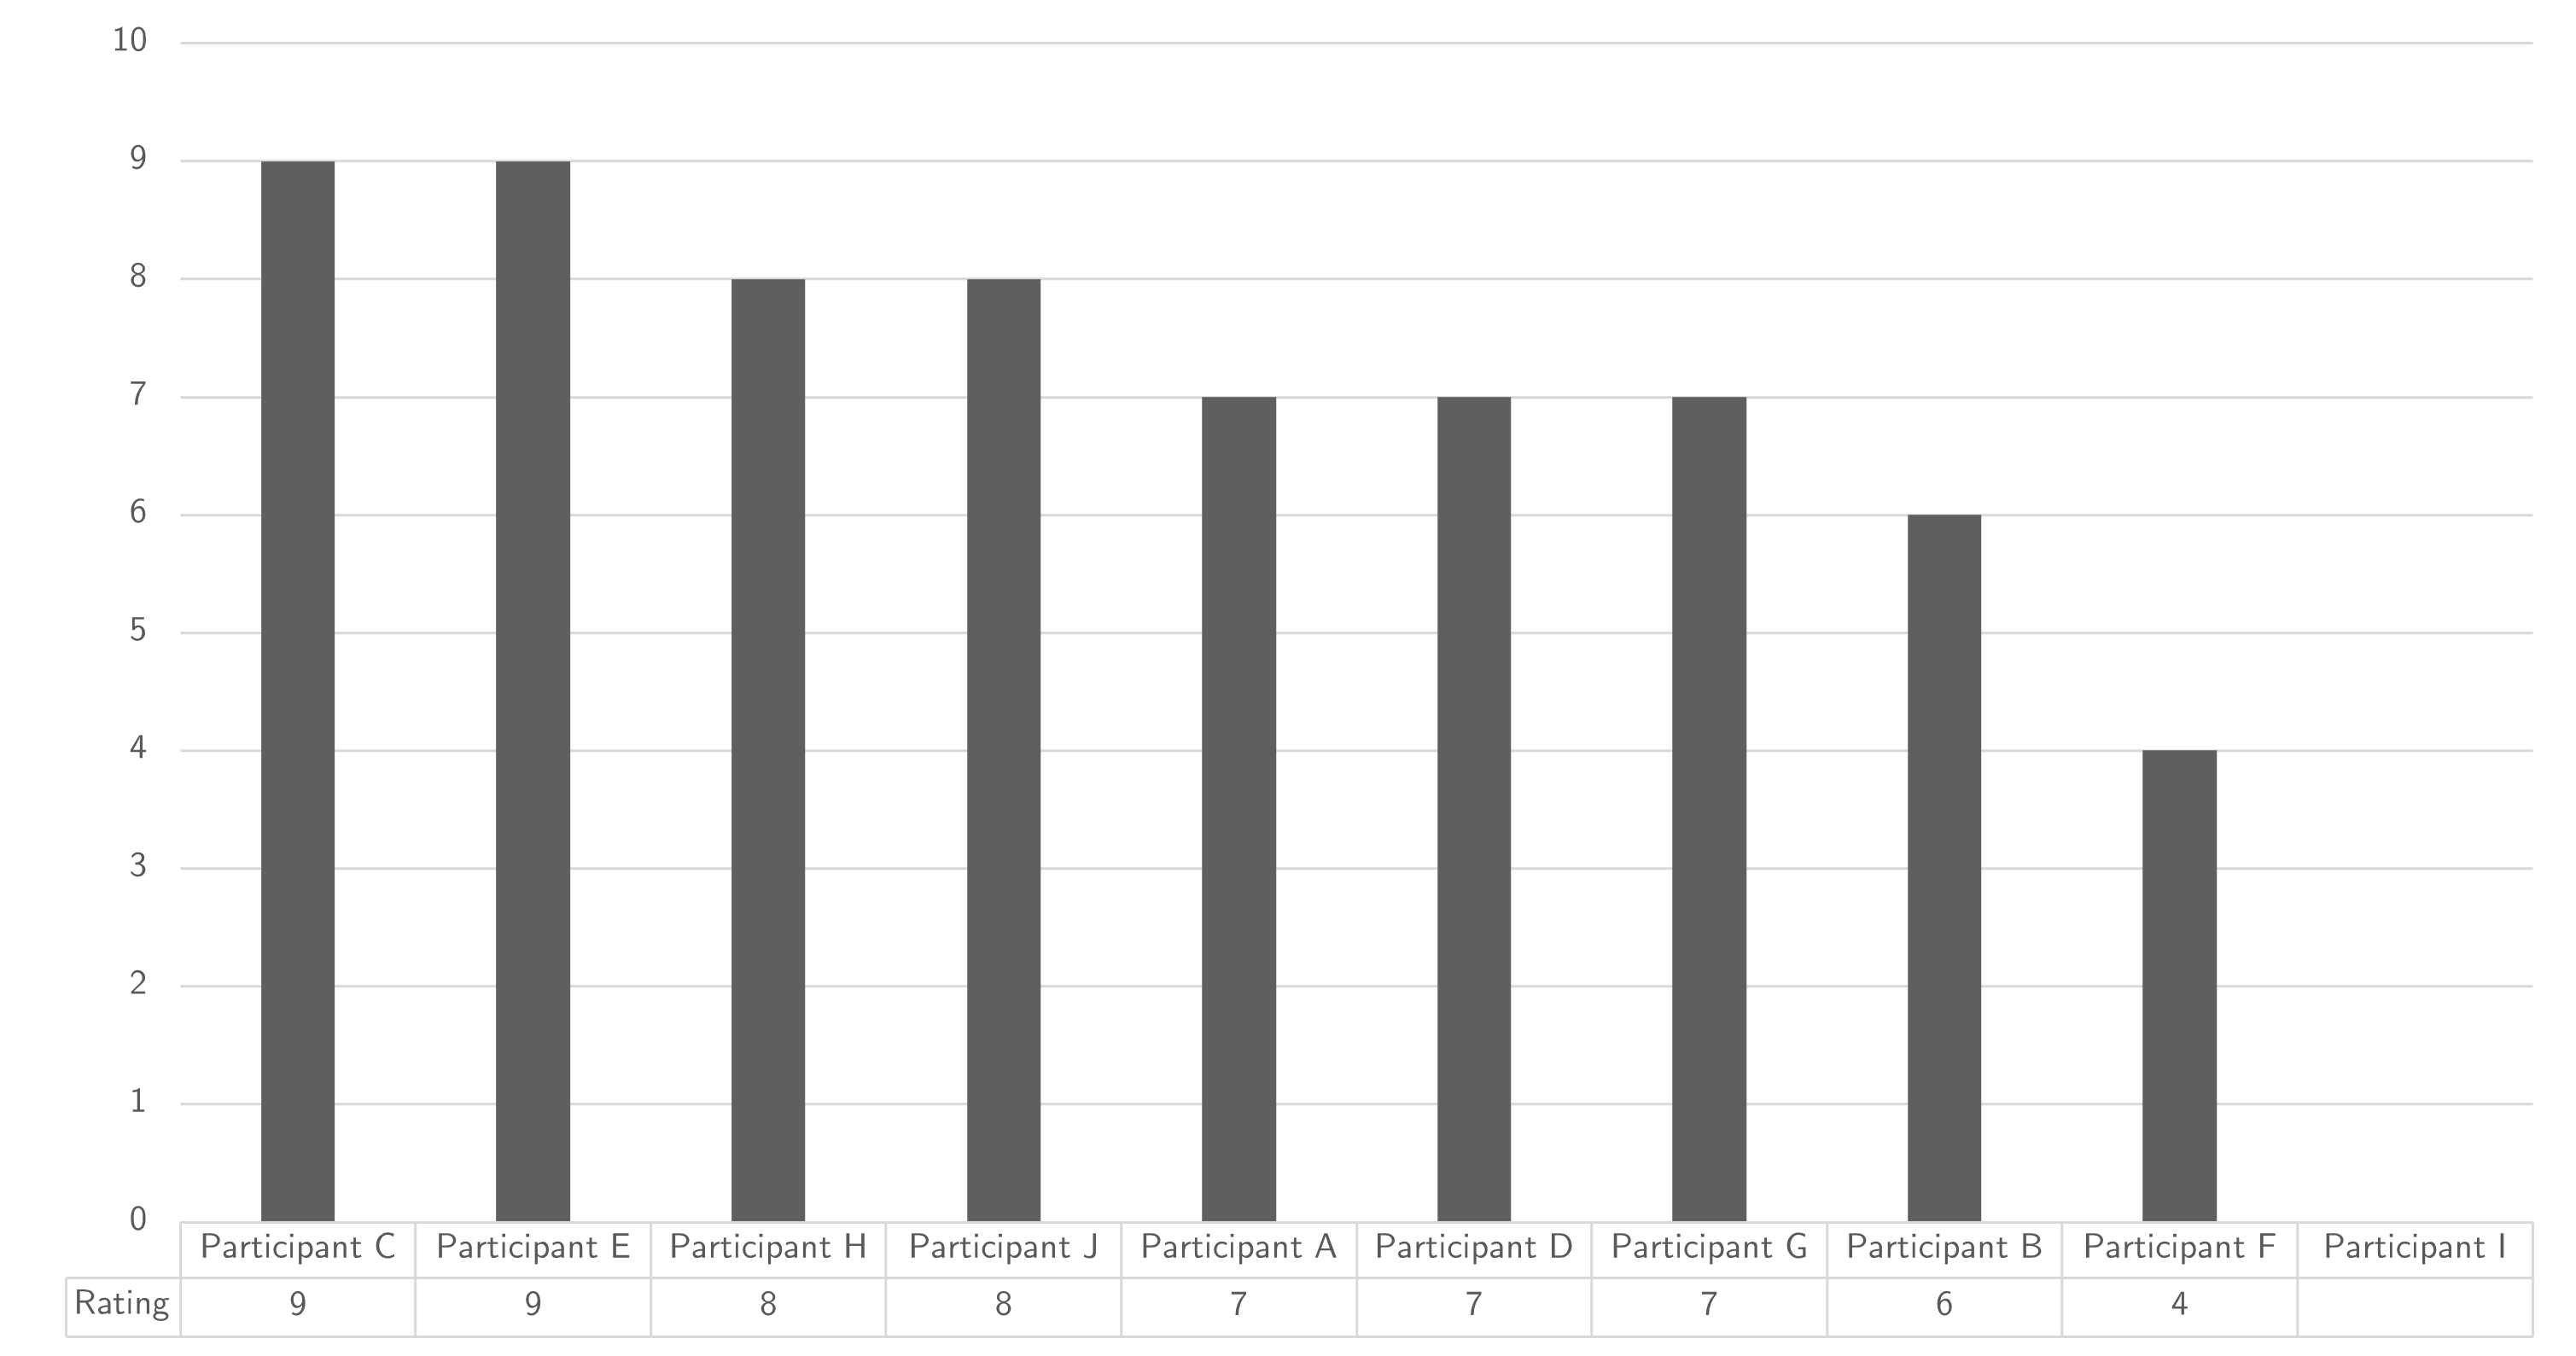
\includegraphics[width=0.9\linewidth]{images/validationresult_researchrelevancepublicsector}
	\caption[To what extent do you think that the research can be used in the public sector?]{To what extent do you think that the research can be used in the public sector?}
	\label{fig:validationrelevantps}
\end{figure}
\begin{table}[H]
	\centering
	\begin{tabular}{p{.55\textwidth}ccc}
		\toprule
		\textbf{Question} & \textbf{Rating} & \textbf{Variability} & \textbf{Abstains} \\
		\midrule
		To what extent do you think that the research can be used in the public sector? & 8,2 & 23\% & 0 \\%
		\bottomrule
	\end{tabular}%
	\caption[To what extent do you think that the research can be used in the public sector?]{To what extent do you think that the research can be used in the public sector?}
	\label{tab:validationrelevantps}%
\end{table}%

\subsection{To what extent do you think that the research can be used by your organisation?}
\label{sub:validationrelevantorganisation}

\begin{figure}[H]
	\centering
	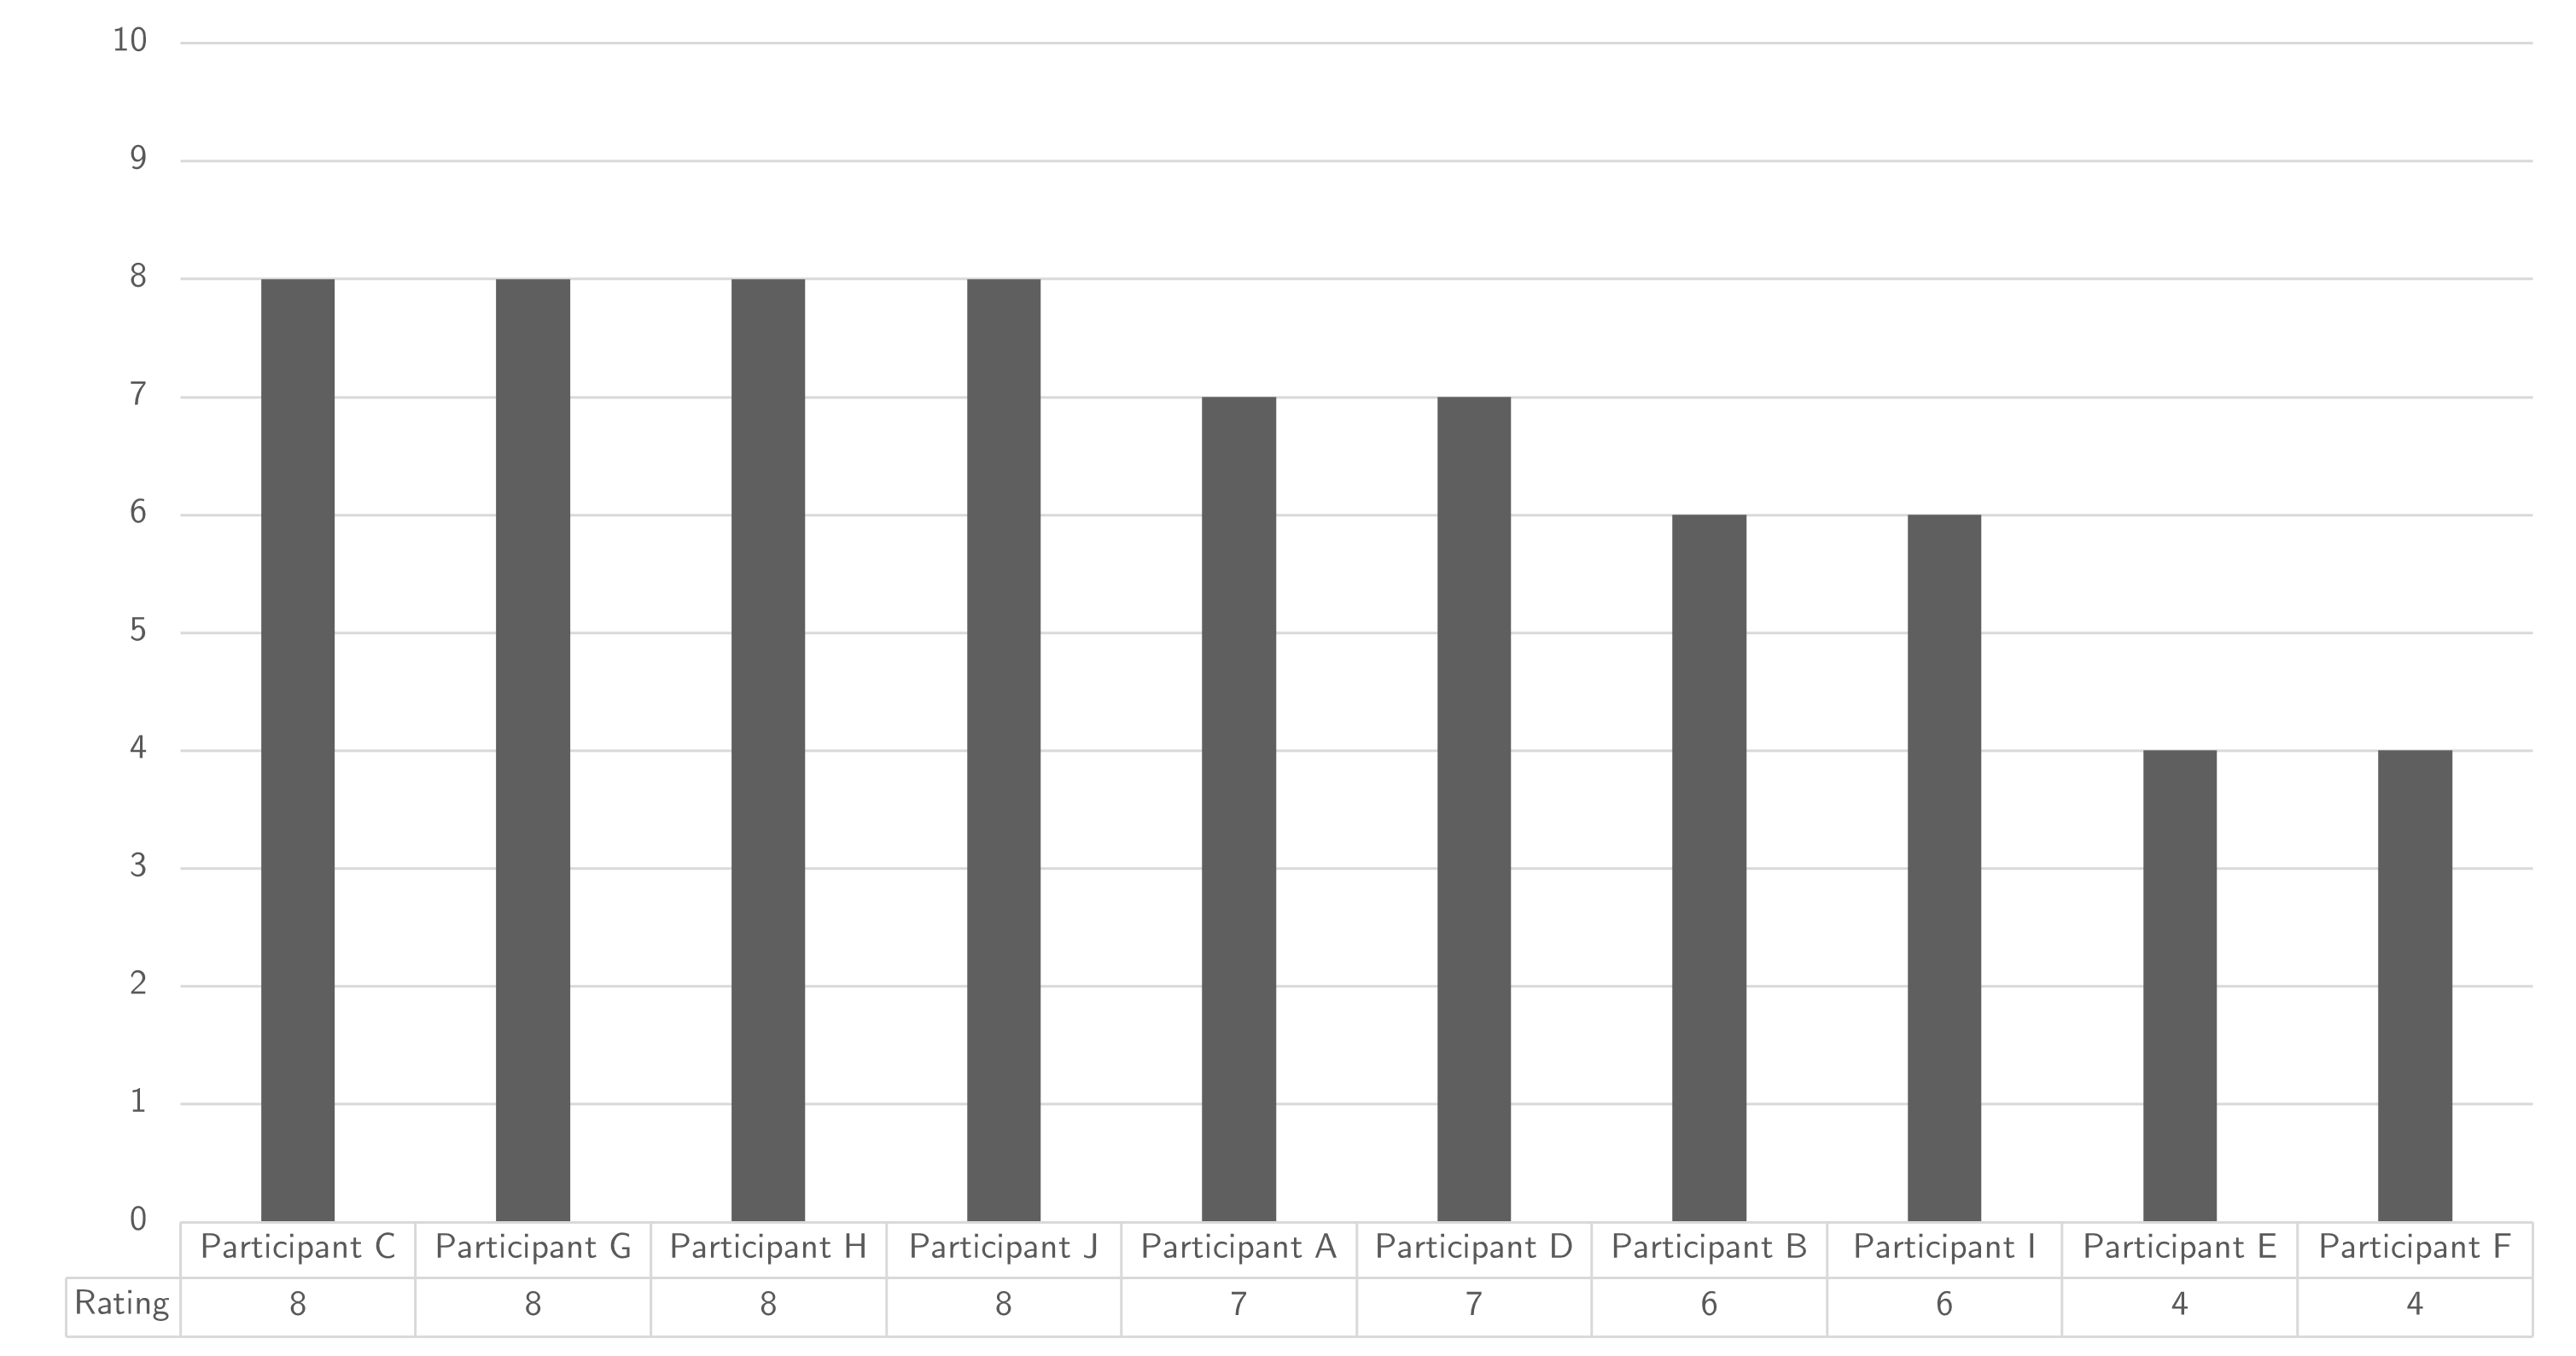
\includegraphics[width=0.9\linewidth]{images/validationresult_researchrelevanceorganisation}
	\caption[To what extent do you think that the research can be used by your organisation?]{To what extent do you think that the research can be used by your organisation?}
	\label{fig:validationrelevantorganisation}
\end{figure}
\begin{table}[H]
	\centering
	\begin{tabular}{p{.55\textwidth}ccc}
		\toprule
		\textbf{Question} & \textbf{Rating} & \textbf{Variability} & \textbf{Abstains} \\
		\midrule
		To what extent do you think that the research can be used by your organisation? & 8,2 & 23\% & 0 \\%
		\bottomrule
	\end{tabular}%
	\caption[To what extent do you think that the research can be used by your organisation?]{To what extent do you think that the research can be used by your organisation?}
	\label{tab:validationrelevantorganisation}%
\end{table}%

\section{Follow-Up Survey}
\begin{table}[H]
	\centering
	\begin{tabular}{p{.55\textwidth}ccc}
		\toprule
		\textbf{Question} & \textbf{Rating} & \textbf{Variability} & \textbf{Abstains} \\
		\midrule
		I want to receive possible updates on this research. & 9 & 0\% & 1 \\%
		I want to know when the thesis is published. & 9 & 0\% & 1 \\%
		\bottomrule
	\end{tabular}%
	\caption{Follow-up Survey}
	\label{tab:appfollowupsurvey}%
\end{table}%